\documentclass{llncs}
\pagestyle{plain}

\usepackage[n,advantage,operators,sets,adversary,landau,probability,notions,
logic,ff,mm,primitives,events,complexity,asymptotics,keys]{cryptocode}
\usepackage{amssymb}
\usepackage{xspace}
\usepackage[normalem]{ulem}
\usepackage{hyperref}
%\usepackage{mathusertools}
\usepackage{multirow}
\usepackage{footnote}
\usepackage{framed}
\usetikzlibrary{decorations.pathreplacing,calligraphy}
\makesavenoteenv{tabular}
\makesavenoteenv{table}

%% Set/unset to activate/deactivate author comments
\def\authnotes{0}

%%% Allows line-breaks in math formulae after commas
\AtBeginDocument{%
  \mathchardef\mathcomma\mathcode`\,
  \mathcode`\,="8000 
}
{\catcode`,=\active
  \gdef,{\mathcomma\discretionary{}{}{}}
}

%%%

\setcounter{tocdepth}{2}

\title{Universal Anonymous Signatures}
\author{Jesus Diaz\inst{1} \and Markulf Kohlweiss\inst{2}}

\institute{Input Output Global,\\
\email{jesus.diazvico@iohk.io},\\
\and
Input Output Global and University of Edinburgh,\\
\email{markulf.kohlweiss@ed.ac.uk}}

% Custom shorthands for this paper
\definecolor{darkgreen}{rgb}{0.1,0.7,0.1}
\newcommand{\todo}[1]{{\colorbox{red}{\bf TODO:}\textcolor{red}{#1}}}
\newcommand{\doubt}[1]{{\colorbox{blue}
    {\textcolor{white}{\bf DOUBT:}}\textcolor{blue}{#1}}}
\newcommand{\response}[1]{{\colorbox{orange}{\bf RESPONSE:}
                                             \textcolor{orange}{#1}}}
\newcommand{\modified}[1]{{\textcolor{orange}{#1}}}
\newcommand{\commentwho}[2]{{\colorbox{darkgreen}{{\bf #1:}}
    \textcolor{darkgreen}{#2}}}
\newcommand{\comment}[1]{{\textcolor{orange}{\# #1}}}
%\newcommand{\note}[1]{{\colorbox{gray}{\bf NOTE:}\textcolor{gray} {#1}}}
\newcommand{\needcite}{[\colorbox{red}{?}]}
\newcommand{\figref}[1]{Fig. \ref{#1}}
\newcommand{\tabref}[1]{Table \ref{#1}}
\newcommand{\lstref}[1]{Listing \ref{#1}}
\newcommand{\secref}[1]{Section \ref{#1}}
\newcommand{\appref}[1]{Appendix \ref{#1}}
\newcommand{\defref}[1]{Definition \ref{#1}}

%\renewcommand{\qedsymbol}{$\blacksquare$}
\newcommand{\br}[1]{\ensuremath{\lbrack #1 \rbrack}}
\newcommand{\gen}[1]{\ensuremath{#1}}

\mathchardef\mhyphen="2D

\def\parm{\ensuremath{param}\xspace}
\def\Exp{\ensuremath{\mathsf{Exp}}\xspace}
\def\Adv{\ensuremath{\mathsf{Adv}}\xspace}
\def\status{\ensuremath{\mathsf{st}}\xspace}

% Symbols for GSAC
\def\GSAC{\ensuremath{\mathsf{GSAC}}\xspace}
\def\HUGEN{\ensuremath{\mathsf{HUGEN}}\xspace}
\def\CUGEN{\ensuremath{\mathsf{CUGEN}}\xspace}
\def\OBTAIN{\ensuremath{\mathsf{OBTAIN}}\xspace}
\def\OBTISS{\ensuremath{\mathsf{OBTISS}}\xspace}
\def\ISSUE{\ensuremath{\mathsf{ISSUE}}\xspace}
\def\SIGN{\ensuremath{\mathsf{SIGN}}\xspace}
\def\OPEN{\ensuremath{\mathsf{OPEN}}\xspace}
\def\CHALb{\ensuremath{\mathsf{CHAL}_b}\xspace}
\def\ATTR{\ensuremath{\mathsf{ATTR}}\xspace}
\def\OWNR{\ensuremath{\mathsf{OWNR}}\xspace}
\def\CRED{\ensuremath{\mathsf{CRED}}\xspace}
\def\USK{\ensuremath{\mathsf{\MakeUppercase{\usk}}}\xspace}
\def\PUBUSK{\ensuremath{\mathsf{P}\USK}\xspace}
\def\PRVUSK{\ensuremath{\mathsf{S}\USK}\xspace}
\def\HU{\ensuremath{\mathsf{HU}}\xspace}
\def\CU{\ensuremath{\mathsf{CU}}\xspace}
\def\SIG{\ensuremath{\mathsf{SIG}}\xspace}
\def\CSIG{\ensuremath{\mathsf{CSIG}}\xspace}
\def\CCRED{\ensuremath{\mathsf{CC}}\xspace}
\def\secpar{\ensuremath{\kappa}\xspace}
\def\param{\ensuremath{\param}\xspace}
\def\isk{\ensuremath{isk}\xspace}
\def\ipk{\ensuremath{ipk}\xspace}
\def\osk{\ensuremath{osk}\xspace}
\def\opk{\ensuremath{opk}\xspace}
\def\gpk{\ensuremath{gpk}\xspace}
\def\usk{\ensuremath{usk}\xspace}
\def\upk{\ensuremath{upk}\xspace}
\def\Attrs{\ensuremath{A}\xspace}
\def\DAttrs{\ensuremath{D}\xspace}
\def\cred{\ensuremath{cred}\xspace}
\def\utrans{\ensuremath{reg}\xspace}
\def\trans{\ensuremath{\MakeUppercase{reg}}\xspace}  
\def\msg{\ensuremath{m}\xspace}
\def\sig{\ensuremath{\sigma}\xspace}
\def\oproof{\ensuremath{\pi}\xspace}
\def\Setup{\ensuremath{Setup}\xspace}
\def\IKeyGen{\ensuremath{IKG}\xspace}
\def\OKeyGen{\ensuremath{OKG}\xspace}
\def\UKeyGen{\ensuremath{UKG}\xspace}
\def\Obtain{\ensuremath{Obtain}\xspace}
\def\Issue{\ensuremath{Issue}\xspace}
\def\Sign{\ensuremath{Sign}\xspace}
\def\Verify{\ensuremath{Verify}\xspace}
\def\Open{\ensuremath{Open}\xspace}
\def\Judge{\ensuremath{Judge}\xspace}
\def\ExpCorrect{\ensuremath{\Exp_{\GSAC,\adv}^{corr}}\xspace}
\def\ExpAnonb{\ensuremath{\Exp_{\GSAC,\adv}^{anon-b}}\xspace}
\def\ExpAnonz{\ensuremath{\Exp_{\GSAC,\adv}^{anon-0}}\xspace}
\def\ExpAnono{\ensuremath{\Exp_{\GSAC,\adv}^{anon-1}}\xspace}
\def\AdvAnon{\ensuremath{\Adv_{\GSAC,\adv}^{anon}}\xspace}
\def\ExpTrace{\ensuremath{\Exp_{\GSAC,\adv}^{trace}}\xspace}
\def\AdvTrace{\ensuremath{\Adv_{\GSAC,\adv}^{trace}}\xspace}
\def\ExpNonframe{\ensuremath{\Exp_{\GSAC,\adv}^{frame}}\xspace}
\def\AdvNonframe{\ensuremath{\Adv_{\GSAC,\adv}^{frame}}\xspace}
\def\choose{\ensuremath{\mathsf{choose}}\xspace}
\def\guess{\ensuremath{\mathsf{guess}}\xspace}
\def\uid{\ensuremath{\mathsf{uid}}\xspace}
\def\cuid{\ensuremath{\mathsf{uid}^*}\xspace}
\def\cid{\ensuremath{\mathsf{cid}}\xspace}
\def\ccid{\ensuremath{\mathsf{cid}^*}\xspace}
\def\csig{\ensuremath{\mathsf{\sigma}^*}\xspace}


%%% Local Variables: 
%%% mode: pdflatex
%%% TeX-master: "gsac.tex"
%%% End:

% Symbols for GSAC
\def\GSAC{\ensuremath{\mathsf{GSAC}}\xspace}
\def\WREG{\ensuremath{\mathsf{WREG}}\xspace}
\def\RREG{\ensuremath{\mathsf{RREG}}\xspace}
\def\HUGEN{\ensuremath{\mathsf{HUGEN}}\xspace}
\def\CUGEN{\ensuremath{\mathsf{CUGEN}}\xspace}
\def\OBTAIN{\ensuremath{\mathsf{OBTAIN}}\xspace}
\def\OBTISS{\ensuremath{\mathsf{OBTISS}}\xspace}
\def\ISSUE{\ensuremath{\mathsf{ISSUE}}\xspace}
\def\SIGN{\ensuremath{\mathsf{SIGN}}\xspace}
\def\OPEN{\ensuremath{\mathsf{OPEN}}\xspace}
\def\CHALb{\ensuremath{\mathsf{CHAL}_b}\xspace}
\def\ATTR{\ensuremath{\mathsf{ATTR}}\xspace}
\def\OWNR{\ensuremath{\mathsf{OWNR}}\xspace}
\def\CRED{\ensuremath{\mathsf{CRED}}\xspace}
\def\USK{\ensuremath{\mathsf{\MakeUppercase{\usk}}}\xspace}
\def\PUBUSK{\ensuremath{\mathsf{P}\USK}\xspace}
\def\PRVUSK{\ensuremath{\mathsf{S}\USK}\xspace}
\def\HU{\ensuremath{\mathsf{HU}}\xspace}
\def\CU{\ensuremath{\mathsf{CU}}\xspace}
\def\SIG{\ensuremath{\mathsf{SIG}}\xspace}
\def\CSIG{\ensuremath{\mathsf{CSIG}}\xspace}
\def\CCRED{\ensuremath{\mathsf{CC}}\xspace}
\def\secpar{\ensuremath{\kappa}\xspace}
\def\nattrs{\ensuremath{n}\xspace}
\def\param{\ensuremath{\param}\xspace}
\def\isk{\ensuremath{isk}\xspace}
\def\ipk{\ensuremath{ipk}\xspace}
\def\osk{\ensuremath{osk}\xspace}
\def\opk{\ensuremath{opk}\xspace}
\def\gpk{\ensuremath{gpk}\xspace}
\def\usk{\ensuremath{usk}\xspace}
\def\upk{\ensuremath{upk}\xspace}
\def\Attrs{\ensuremath{\mathsf{A}}\xspace}
\def\DAttrs{\ensuremath{\mathsf{D}}\xspace}
\def\cred{\ensuremath{cred}\xspace}
\def\utrans{\ensuremath{reg}\xspace}
\def\trans{\ensuremath{\MakeUppercase{reg}}\xspace}  
\def\msg{\ensuremath{m}\xspace}
\def\sig{\ensuremath{\sigma}\xspace}
\def\oproof{\ensuremath{\pi}\xspace}
\def\Setup{\ensuremath{Setup}\xspace}
\def\IKeyGen{\ensuremath{IKG}\xspace}
\def\OKeyGen{\ensuremath{OKG}\xspace}
\def\UKeyGen{\ensuremath{UKG}\xspace}
\def\Obtain{\ensuremath{Obtain}\xspace}
\def\Issue{\ensuremath{Issue}\xspace}
\def\Sign{\ensuremath{Sign}\xspace}
\def\Verify{\ensuremath{Verify}\xspace}
\def\Open{\ensuremath{Open}\xspace}
\def\Judge{\ensuremath{Judge}\xspace}
\def\ExpGSACCorrect{\ensuremath{\Exp_{\GSAC,\adv}^{corr}}\xspace}
\def\ExpGSACAnonb{\ensuremath{\Exp_{\GSAC,\adv}^{anon-b}}\xspace}
\def\ExpGSACAnonz{\ensuremath{\Exp_{\GSAC,\adv}^{anon-0}}\xspace}
\def\ExpGSACAnono{\ensuremath{\Exp_{\GSAC,\adv}^{anon-1}}\xspace}
\def\AdvGSACAnon{\ensuremath{\Adv_{\GSAC,\adv}^{anon}}\xspace}
\def\ExpGSACTrace{\ensuremath{\Exp_{\GSAC,\adv}^{trace}}\xspace}
\def\AdvGSACTrace{\ensuremath{\Adv_{\GSAC,\adv}^{trace}}\xspace}
\def\ExpGSACNonframe{\ensuremath{\Exp_{\GSAC,\adv}^{frame}}\xspace}
\def\AdvGSACNonframe{\ensuremath{\Adv_{\GSAC,\adv}^{frame}}\xspace}
\def\choose{\ensuremath{\mathsf{choose}}\xspace}
\def\guess{\ensuremath{\mathsf{guess}}\xspace}
\def\uid{\ensuremath{\mathsf{uid}}\xspace}
\def\cuid{\ensuremath{\mathsf{uid}^*}\xspace}
\def\cid{\ensuremath{\mathsf{cid}}\xspace}
\def\ccid{\ensuremath{\mathsf{cid}^*}\xspace}
\def\csig{\ensuremath{\mathsf{\sigma}^*}\xspace}
\def\credid{\ensuremath{cid}\xspace}
\def\Ccredid{\ensuremath{\Ccom_{\credid}}\xspace}
\def\Cusk{\ensuremath{\Ccom_{\usk}}\xspace}
\def\attr{\ensuremath{attr}\xspace}

%%% Local Variables: 
%%% mode: pdflatex
%%% TeX-master: "gsac.tex"
%%% End:

% Symbols for UAS
\def\UAS{\ensuremath{\mathsf{UAS}}\xspace}
\def\IGEN{\ensuremath{\mathsf{IGEN}}\xspace}
\def\OGEN{\ensuremath{\mathsf{OGEN}}\xspace}
\def\UGEN{\ensuremath{\mathsf{UGEN}}\xspace}
\def\ICORR{\ensuremath{\mathsf{ICORR}}\xspace}
\def\OCORR{\ensuremath{\mathsf{OCORR}}\xspace}
\def\UCORR{\ensuremath{\mathsf{UCORR}}\xspace}
\def\CCORR{\ensuremath{\mathsf{CCORR}}\xspace}
\def\HUGEN{\ensuremath{\mathsf{HUGEN}}\xspace}
\def\CUGEN{\ensuremath{\mathsf{CUGEN}}\xspace}
\def\ISET{\ensuremath{\mathsf{ISET}}\xspace}
\def\OBTAIN{\ensuremath{\mathsf{OBTAIN}}\xspace}
\def\OBTISS{\ensuremath{\mathsf{OBTISS}}\xspace}
\def\ISSUE{\ensuremath{\mathsf{ISSUE}}\xspace}
\def\SIGN{\ensuremath{\mathsf{SIGN}}\xspace}
\def\OPEN{\ensuremath{\mathsf{OPEN}}\xspace}
\def\INSPECT{\ensuremath{\mathsf{INSPECT}}\xspace}
\def\CHALb{\ensuremath{\mathsf{SIGCHAL}_b}\xspace}
\def\OBTCHALb{\ensuremath{\mathsf{OBTCHAL}_b}\xspace}
\def\SIMSETUP{\ensuremath{\mathsf{SimSetup}}\xspace}
\def\SIMOBTAIN{\ensuremath{\mathsf{SIMOBTAIN}}\xspace}
\def\SIMSIGN{\ensuremath{\mathsf{SIMSIGN}}\xspace}
\def\SIMOPEN{\ensuremath{\mathsf{SIMOPEN}}\xspace}
\def\ATTR{\ensuremath{\mathsf{ATT}}\xspace}
\def\UATTR{\ensuremath{\mathsf{U}\ATTR}\xspace}
\def\DATTR{\ensuremath{\mathsf{D}\ATTR}\xspace}
\def\OWNR{\ensuremath{\mathsf{OWN}}\xspace}
\def\GRP{\ensuremath{\mathsf{GRP}}\xspace}
\def\ISR{\ensuremath{\mathsf{ISR}}\xspace}
\def\CCRED{\ensuremath{\mathsf{CCRD}}\xspace}
\def\IK{\ensuremath{\mathsf{IK}}\xspace}
\def\OK{\ensuremath{\mathsf{OK}}\xspace}
\def\UK{\ensuremath{\mathsf{UK}}\xspace}
\def\GK{\ensuremath{\mathsf{GK}}\xspace}
\def\PUBIK{\ensuremath{\mathsf{P}\IK}\xspace}
\def\PRVIK{\ensuremath{\mathsf{S}\IK}\xspace}
\def\PUBOK{\ensuremath{\mathsf{P}\OK}\xspace}
\def\PRVOK{\ensuremath{\mathsf{S}\OK}\xspace}
\def\PUBUK{\ensuremath{\mathsf{P}\UK}\xspace}
\def\PRVUK{\ensuremath{\mathsf{S}\UK}\xspace}
\def\II{\ensuremath{\mathsf{I}}\xspace}
\def\OO{\ensuremath{\mathsf{O}}\xspace}
\def\UU{\ensuremath{\mathsf{U}}\xspace}
\def\HI{\ensuremath{\mathsf{HI}}\xspace}
\def\CI{\ensuremath{\mathsf{CI}}\xspace}
\def\HO{\ensuremath{\mathsf{HO}}\xspace}
\def\CO{\ensuremath{\mathsf{CO}}\xspace}
\def\HU{\ensuremath{\mathsf{HU}}\xspace}
\def\CU{\ensuremath{\mathsf{CU}}\xspace}
\def\CC{\ensuremath{\mathsf{CC}}\xspace}
\def\GEN{\ensuremath{\mathsf{GEN}}\xspace}
\def\CORR{\ensuremath{\mathsf{CORR}}\xspace}
\def\SIG{\ensuremath{\mathsf{SIG}}\xspace}
\def\CSIG{\ensuremath{\mathsf{CSIG}}\xspace}
%\def\CCRED{\ensuremath{\mathsf{CC}}\xspace}
\def\secpar{\ensuremath{\kappa}\xspace}
%\def\param{\ensuremath{\param}\xspace}
\def\isk{\ensuremath{isk}\xspace}
\def\ipk{\ensuremath{ipk}\xspace}
\def\sipk{\ensuremath{\mathbf{\ipk}}\xspace}
\def\osk{\ensuremath{osk}\xspace}
\def\opk{\ensuremath{opk}\xspace}
\def\gpk{\ensuremath{gpk}\xspace}
\def\sgpk{\ensuremath{\mathbf{\gpk}}\xspace}
\def\usk{\ensuremath{usk}\xspace}
\def\upk{\ensuremath{upk}\xspace}
\def\uk{\ensuremath{uk}\xspace}
\def\Cred{\ensuremath{C}\xspace}
\def\sCred{\ensuremath{\mathbf{C}}\xspace}
\def\credid{\ensuremath{cid}\xspace}
\def\scredid{\ensuremath{\boldsymbol{cid}}\xspace}
\def\cred{\ensuremath{crd}\xspace}
\def\scred{\ensuremath{\mathbf{\cred}}\xspace}
\def\utrans{\ensuremath{reg}\xspace}
\def\trans{\ensuremath{\mathbf{reg}}\xspace}
\def\IdentifyCred{\ensuremath{\mathsf{IdentifyCred}}\xspace}
\def\IdentifySig{\ensuremath{\mathsf{IdentifySig}}\xspace}
\def\ExtractSetup{\ensuremath{\mathsf{ExtSetup}}\xspace}
\def\ExtractSign{\ensuremath{\mathsf{ExtSign}}\xspace}
\def\ExtractIssue{\ensuremath{\mathsf{ExtIss}}\xspace}
\def\c{\ensuremath{c}\xspace}
\def\y{\ensuremath{y}\xspace}
\def\yissue{\ensuremath{y_{is}}\xspace}
\def\yeval{\ensuremath{y_{ev}}\xspace}
\def\tyeval{\ensuremath{\tilde{y}_{ev}}\xspace}
\def\ceval{\ensuremath{\c_{ev}}\xspace}
\def\Yeval{\ensuremath{Y_{ev}}\xspace}
\def\TYeval{\ensuremath{\tilde{Y}_{ev}}\xspace}
\def\yinsp{\ensuremath{y_{op}}\xspace}
\def\tyinsp{\ensuremath{\tilde{y}_{op}}\xspace}
\def\cinsp{\ensuremath{\c_{op}}\xspace}
\def\sig{\ensuremath{\sigma}\xspace}
\def\Sig{\ensuremath{\Sigma}\xspace}
\def\iproof{\ensuremath{\pi}\xspace}
\def\tiproof{\ensuremath{\tilde{\pi}}\xspace}
\def\Setup{\ensuremath{Setup}\xspace}
\def\KeyGen{\ensuremath{KG}\xspace}
\def\IKeyGen{\ensuremath{IKG}\xspace}
\def\OKeyGen{\ensuremath{OKG}\xspace}
\def\UKeyGen{\ensuremath{UKG}\xspace}
\def\ISet{\ensuremath{ISet}\xspace}
\def\Obtain{\ensuremath{Obt}\xspace}
\def\Issue{\ensuremath{Iss}\xspace}
\def\Sign{\ensuremath{Sign}\xspace}
\def\Verify{\ensuremath{Verify}\xspace}
\def\Inspect{\ensuremath{Inspect}\xspace}
\def\Judge{\ensuremath{Judge}\xspace}
\def\ExpCorrect{\ensuremath{\Exp_{\UAS,\adv}^{corr}}\xspace}
\def\CorrectIssue{\ensuremath{CorrectIssue}\xspace}
\def\CorrectEval{\ensuremath{CorrectEval}\xspace}
\def\CorrectEvalInspect{\ensuremath{CorrectEvalInspect}\xspace}
\def\CorrectInspect{\ensuremath{CorrectInspect}\xspace}
\def\ExpExtractIssue{\ensuremath{\Exp_{\UAS,\adv}^{ext-iss}}\xspace}
\def\ExpExtractSign{\ensuremath{\Exp_{\UAS,\adv}^{ext-sig}}\xspace}
\def\ExpIdentifyCred{\ensuremath{\Exp_{\UAS,\adv}^{id-cred}}\xspace}
\def\ExpIdentifySign{\ensuremath{\Exp_{\UAS,\adv}^{id-sig}}\xspace}
\def\ExpSimAnonb{\ensuremath{\Exp_{\UAS,\adv}^{sim-anon-b}}\xspace}
\def\ExpSigAnonb{\ensuremath{\Exp_{\UAS,\adv}^{sig-anon-b}}\xspace}
\def\ExpIssAnonb{\ensuremath{\Exp_{\UAS,\adv}^{iss-anon-b}}\xspace}
\def\ExpSigAnonz{\ensuremath{\Exp_{\UAS,\adv}^{sig-anon-0}}\xspace}
\def\ExpIssAnonz{\ensuremath{\Exp_{\UAS,\adv}^{iss-anon-0}}\xspace}
\def\ExpSigAnonzo{\ensuremath{\Exp_{\UAS,\adv}^{sig-anon-01}}\xspace}
\def\ExpSigAnono{\ensuremath{\Exp_{\UAS,\adv}^{sig-anon-1}}\xspace}
\def\ExpIssAnono{\ensuremath{\Exp_{\UAS,\adv}^{iss-anon-1}}\xspace}
\def\ExpSigAnonoz{\ensuremath{\Exp_{\UAS,\adv}^{sig-anon-10}}\xspace}
\def\ExpSimAnono{\ensuremath{\Exp_{\UAS,\adv}^{sim-anon-1}}\xspace}
\def\ExpSimAnonz{\ensuremath{\Exp_{\UAS,\adv}^{sim-anon-0}}\xspace}
\def\AdvSigAnon{\ensuremath{\Adv_{\UAS,\adv}^{sig-anon}}\xspace}
\def\AdvIssAnon{\ensuremath{\Adv_{\UAS,\adv}^{iss-anon}}\xspace}
\def\AdvSimAnon{\ensuremath{\Adv_{\UAS,\adv}^{sim-anon}}\xspace}
\def\AdvIdCred{\ensuremath{\Adv_{\UAS,\adv}^{id-cred}}\xspace}
\def\AdvIdSign{\ensuremath{\Adv_{\UAS,\adv}^{id-sig}}\xspace}
\def\ExpTrace{\ensuremath{\Exp_{\UAS,\adv}^{trace}}\xspace}
\def\AdvTrace{\ensuremath{\Adv_{\UAS,\adv}^{trace}}\xspace}
\def\IssueTrace{\ensuremath{IssTrace}\xspace}
\def\IssueForge{\ensuremath{IssForge}\xspace}
\def\ExpForge{\ensuremath{\Exp_{\UAS,\adv}^{forge}}\xspace}
\def\ExpForgeIssue{\ensuremath{\Exp_{\UAS,\adv}^{iss-forge}}\xspace}
\def\AdvForge{\ensuremath{\Adv_{\UAS,\adv}^{forge}}\xspace}
\def\AdvForgeIssue{\ensuremath{\Adv_{\UAS,\adv}^{iss-forge}}\xspace}
\def\ExpForgeSign{\ensuremath{\Exp_{\UAS,\adv}^{sig-forge}}\xspace}
\def\AdvForgeSign{\ensuremath{\Adv_{\UAS,\adv}^{sig-forge}}\xspace}
\def\EvalForge{\ensuremath{EvForge}\xspace}
\def\EvalInspectForge{\ensuremath{EvInForge}\xspace}
\def\InspectForge{\ensuremath{InForge}\xspace}
\def\ExpNonframe{\ensuremath{\Exp_{\UAS,\adv}^{frame}}\xspace}
\def\AdvNonframe{\ensuremath{\Adv_{\UAS,\adv}^{frame}}\xspace}
\def\ExpNonframeSign{\ensuremath{\Exp_{\UAS,\adv}^{frame-sign}}\xspace}
\def\AdvNonframeSign{\ensuremath{\Adv_{\UAS,\adv}^{frame-insp}}\xspace}
\def\ExpNonframeInsp{\ensuremath{\Exp_{\UAS,\adv}^{frame-insp}}\xspace}
\def\AdvNonframeInsp{\ensuremath{\Adv_{\UAS,\adv}^{frame-insp}}\xspace}
\def\ExpExtractIssue{\ensuremath{\Exp_{\UAS,\adv}^{ext-issue}}\xspace}
\def\AdvExtractIssue{\ensuremath{\Adv_{\UAS,\adv}^{ext-issue}}\xspace}
\def\ExpExtractSign{\ensuremath{\Exp_{\UAS,\adv}^{ext-sign}}\xspace}
\def\AdvExtractSign{\ensuremath{\Adv_{\UAS,\adv}^{ext-sign}}\xspace}
\def\choose{\ensuremath{\mathsf{choose}}\xspace}
\def\guess{\ensuremath{\mathsf{guess}}\xspace}
\def\Oanonc{\ensuremath{\mathcal{O}_{anon-b}_{\choose}}\xspace}
\def\Oanong{\ensuremath{\mathcal{O}_{anon-b}_{\guess}}\xspace}
\def\OExt{\ensuremath{\mathcal{O}_{ext}}\xspace}
\def\OId{\ensuremath{\mathcal{O}_{id}}\xspace}
\def\OAnon{\ensuremath{\mathcal{O}_{anon-b}}\xspace}
\def\OIssAnon{\ensuremath{\mathcal{O}_{iss-anon-b}}\xspace}
\def\OSigAnon{\ensuremath{\mathcal{O}_{sig-anon-b}}\xspace}
\def\Osimanon{\ensuremath{\mathcal{O}_{sim-anon-b}}\xspace}
\def\Otrace{\ensuremath{\mathcal{O}_{trace}}\xspace}
\def\Oforge{\ensuremath{\mathcal{O}_{forge}}\xspace}
\def\Oforgeissue{\ensuremath{\mathcal{O}_{iss-forge}}\xspace}
\def\Oforgesign{\ensuremath{\mathcal{O}_{sig-forge}}\xspace}
\def\Oframe{\ensuremath{\mathcal{O}_{frame}}\xspace}
\def\gid{\ensuremath{\mathsf{gid}}\xspace}
\def\iid{\ensuremath{\mathsf{iid}}\xspace}
\def\oid{\ensuremath{\mathsf{oid}}\xspace}
\def\sgid{\ensuremath{\boldsymbol{\mathsf{\gid}}}\xspace}
\def\siid{\ensuremath{\boldsymbol{\mathsf{\iid}}}\xspace}
\def\uid{\ensuremath{\mathsf{uid}}\xspace}
\def\suid{\ensuremath{\boldsymbol{\mathsf{uid}}}\xspace}
\def\cuid{\ensuremath{\mathsf{uid}^*}\xspace}
\def\cid{\ensuremath{cid}\xspace}
\def\cidi{\ensuremath{cid^I}\xspace}
\def\cidu{\ensuremath{cid^U}\xspace}
\def\scid{\ensuremath{\boldsymbol{cid}}\xspace}
\def\ccid{\ensuremath{cid^*}\xspace}
\def\ccidi{\ensuremath{cid^{I*}}\xspace}
\def\ccidu{\ensuremath{cid^{U*}}\xspace}
\def\cscid{\ensuremath{\scid^*}\xspace}
\def\csig{\ensuremath{\mathsf{\sigma}^*}\xspace}
\def\cSig{\ensuremath{\mathsf{\Sigma}^*}\xspace}
\def\LangIss{\ensuremath{\Lang_{iss}}\xspace}
\def\RelIss{\ensuremath{\NIZKRel_{iss}}\xspace}
\def\LangIns{\ensuremath{\Lang_{op}}\xspace}
\def\RelIns{\ensuremath{\NIZKRel_{op}}\xspace}
\def\LangVerIns{\ensuremath{\Lang_{verop}}\xspace}
\def\LangSig{\ensuremath{\Lang_{sig}}\xspace}
\def\RelSig{\ensuremath{\NIZKRel_{sig}}\xspace}
\def\fissue{\ensuremath{f_{is}}\xspace}
\def\rngfissue{\ensuremath{R_{is}}\xspace}
\def\feval{\ensuremath{f_{ev}}\xspace}
\def\rngfeval{\ensuremath{R_{ev}}\xspace}
\def\varrngfeval{\ensuremath{r_{ev}}\xspace}
\def\finsp{\ensuremath{f_{op}}\xspace}
\def\rngfinsp{\ensuremath{R_{op}}\xspace}
\def\varrngfinsp{\ensuremath{r_{op}}\xspace}
\def\famfissue{\ensuremath{\mathcal{F}_{is}}\xspace}
\def\famfeval{\ensuremath{\mathcal{F}_{ev}}\xspace}
\def\famfinsp{\ensuremath{\mathcal{F}_{op}}\xspace}
\def\Issuers{\ensuremath{\mathbb{I}}\xspace}
\def\CUASGen{\ensuremath{\Pi_{\UAS}}\xspace}
\def\CUASGenHideIss{\ensuremath{\CUASGen^{hide-iss}}\xspace}
\def\CUASGenInt{\ensuremath{\CUASGen^{int}}\xspace}
\def\trap{\ensuremath{\tau}\xspace}
\def\extract{\ensuremath{\mathsf{ex}}\xspace}
\def\extracttrap{\ensuremath{\tau_{\extract}}\xspace}
\def\sring{\ensuremath{\mathbf{ring}}\xspace}
\def\CUASRing{\ensuremath{\Pi_{\UAS}^{ring}}\xspace}
\def\CUASGS{\ensuremath{\Pi_{\UAS}^{gs}}\xspace}
\def\CUASAC{\ensuremath{\Pi_{\UAS}^{ac}}\xspace}
\def\CUASGSMDO{\ensuremath{\Pi_{\UAS}^{gsmdo}}\xspace}
\def\CUASDAC{\ensuremath{\Pi_{\UAS}^{dac}}\xspace}
\def\CUASRAC{\ensuremath{\Pi_{\UAS}^{rac}}\xspace}
\def\CUASMPS{\ensuremath{\Pi_{\UAS}^{mps}}\xspace}
\def\proofins{\ensuremath{\NIZKproof_{op}}\xspace}
\def\proofsig{\ensuremath{\NIZKproof_{sig}}\xspace}
\def\crsiss{\ensuremath{\NIZKcrs_{iss}}\xspace}
\def\crssig{\ensuremath{\NIZKcrs_{sig}}\xspace}
\def\crsins{\ensuremath{\NIZKcrs_{op}}\xspace}

%%% Local Variables: 
%%% mode: pdflatex
%%% TeX-master: "gsac.tex"
%%% End:


\begin{document}
{\def\addcontentsline#1#2#3{}\maketitle}%\maketitle
\ifnum\authnotes=1
Version of \today
\fi

\begin{abstract}
  For decades, anonymous credentials, group signatures, and closely related
  systems in the domain of privacy-preserving authentication, have relied on
  common cryptographic building blocks. However, each has its own approach
  modelling-wise, despite obvious commonalities.
  %
  Even within systems of the same type, multiple ``sub-models'' and
  constructions coexist that cater for slightly different requirements.

  Previous works, like Camenisch et al in SAC'15, or Nguyen et al in CRYPTO'22
  generalize aspects of those systems, but still within their own domain --
  anonymous credentials and group signatures, respectively.

  In this work, we make a significant generalization effort in order to come
  up with a flexible game-based model that subsumes
  previous ones. The key to this flexibility lies in functional placeholders
  that, with careful constraints, still allow to capture generalized notions of
  the usual anonymity, unforgeability and non-frameability properties. We refer
  to this unified model as \emph{Universal Anonymous Signatures} (\UAS).

  To showcase the generality of \UAS, we give a main construction, plus two
  alternative ones that slightly modify it, following our \UAS model.
  We prove that, from these constructions, we can build multiple variants of
  group signatures, anonymous credentials, and ring signatures, just by giving
  concrete definitions of the mentioned functional placeholders.
  
  Our main theoretical contribution is unifying previously separate
  (albeit close) systems under the same generalized model. Indeed, such unified
  model allows to, very easily, build ``hybrid'' systems that combine features
  of previously separately modelled constructions: e.g., anonymous credentials
  with conditional deanonymization based on their attributes.
  
  More practically, this has the consequence that cryptographic
  engineers and system designers can tweak the desired utility-vs-privacy
  tradeoff that best suits their needs, just by defining a few functions --
  but without needing to prove security from scratch or implement
  a whole system.
\end{abstract}

\section{Introduction}
\label{sec:introduction}

% [4 pages max]

%% Brief description of main precedents (simple words)
\paragraph{Anonymous authentication and signatures.} %
Privacy-preserving digital signature and authentication systems have been a
prolific field of study in the last few decades. Anonymous credentials
\cite{chau85} and group signatures \cite{ch91} are among the most relevant ones.
While there are many variants, the high-level idea is common: after obtaining a
credential, users can authenticate anonymously and indistinguishably from other
users with similar credentials. 

%% Usefulness of main precedents / motivation
Their usefulness stems from the combination, within a single primitive, of
seemingly contradictory concepts: anonymity, authentication, and utility; where
utility can appear in the shape of information revealed at signature/authentication
time, or after (in the latter case, typically called accountability).

\paragraph{Utility at authentication-time and after authentication-time.} %
Anonymous credentials (AC) focus on utility at authentication time. For
instance, encoding multiple attributes within a credential and allowing to
selectively disclose a subset of them, or even arbitrary predicates.
The real world applications of such systems are direct,
e.g., to prove ``Over 18''-type of claims. Indeed, the scientific research
behind anonymous credentials is making its own way to become a foundational
block of the technology some call ``anoncreds''%
\footnote{\url{https://hyperledger-indy.readthedocs.io/projects/sdk/en/latest/docs/design/002-anoncreds/README.html}. Last access, June 18th, 2022.},
the privacy-preserving cousin of W3C's Verifiable Credentials%
\footnote{\url{https://www.w3.org/TR/vc-data-model/}. Last access, June 18th,
  2022.}.

Group signatures (GS) enhance utility after authentication, by allowing partial
reidentification like linking of signatures, or even full deanonymization.
While actual applications of group signatures seem hard to find in the real
world, Direct Anonymous Attestation (DAA) \cite{bcc04,bl07,cdl16b} has been deployed to
millions of computing devices into what's called TPM (Trusted Privacy Module)%
\footnote{\url{https://trustedcomputinggroup.org/resource/trusted-platform-module-tpm-summary/}. Last access, June 18th, 2022.}.
Indeed, DAA is a very close relative of group signatures, where the signer is
divided into two components (trusted and partially trusted), and signing
and verification are turned into an interactive protocol.

%% Previous works summary w/ refs directly related contribs of UAS
%% (or, tech approaches of main precedents)
\paragraph{Evolution of AC and GS.} %
As the previous shows, AC and GS systems have followed separate paths, although
there are some exceptions. Functionality-wise, Attribute-Based Group Signatures
(ABGS) introduce attributes into the credentials issued to group members, who
can later use them to prove pre-fixed claims \cite{emo09,aa14}. Hidden-identity
signatures also add attributes into the credentials, with the aim of preventing
the opener (the trusted party who can deanonymize signers) from having to rely
on the issuer in order to perform the opening \cite{ks07}. Some AC schemes have
also tried to incorporate some sort of utility after authentication, like AC
schemes with revocation \cite{cks10}, or with ``watchlists'' \needcite.

This separation does not hold in the approaches to build them, though. The
probably most fruitful way to design and instantiate AC systems
is with CL-type signatures \cite{cl02}. But the fact that they support efficient
zero-knowledge protocols for proving knowledge of a signature, makes them very
suitable to build GS schemes -- even without exploiting the possibility to
encode many attributes. Indeed, BBS+ signatures \cite{bbs04,cdl16b} have been
used to design and instantiate GS schemes \cite{gl19,dl21}, as well as  PS16
signatures \cite{ps16,cdl+20}. Both are CL-like signature schemes, and thus
can be (and have been) used to design AC schemes \needcite.

Also, both AC and GS branches have experienced praiseworthy efforts towards
generalization. In the AC domain, malleable signatures are used as core building
block in \cite{cklm14}, to allow building both conventional AC and Delegatable
AC systems, depending on the transformation supported by the malleable
signatures. In GS, very recently, BiAS \cite{lnpy21} and MPS \needcite
flexibilize the tradeoff between anonymity and accountability.

%% Main drawbacks of precedents
\paragraph{Limitations of GS and AC.} %
However, even the generalization efforts that have independently taken place in
GS and AC, are quickly seen to have limited applicability in the real world.
On the GS side, even though MPS achieves a nice balance on when a signature is
deanonymizable and what information can be extracted from it, upon closer look,
this information is somehow meaningless. To understand it, consider how does the
generic construction work. Roughly, the signer encrypts the output of an
arbitrary function of its ``identity'', and proves correctness of this
computation. Yet, the concept of ``identity'' is not defined at all (it is a
value within some undefined domain). Thus, it seems hard to associate any real
world meaning to a function of something that is not clearly defined. In any
case, proving membership to a group may be enough in some use cases, but
definitely not as a general tool -- that is, GS  offer minimal utility at
signing time.
%
On the other hand, ACs have a well defined concept of identity (the attributes
encoded within a credential), yet their utility-after-authentication
capabilities are 
minimal -- something on which their GS counterpart has done decades of research.
A somehow indirect proof of this is that the AC line of work does not even
consider what security we can get in the presence of malicious issuers, which
is precisely captured in the non-frameability properties of GS.

\subsection{Our Contribution} 
%% Our results; TLDR (simple words)

\paragraph{General model for anonymous signatures.} %
Acknowledging that the strengths of AC are the weaknesses of GS, and vice versa,
we come up with a unified model. In a nutshell, we give a sytnax and model for
anonymous signatures -- which can be turned into an interactive authentication
system -- with attribute-enabled credentials, and generalized utility
both at authentication/signature-time, and after. We also generalize the
credential issuance process, subsuming an even larger set of previously
known schemes. Given its generalization power, we refer to schemes meeting this
model as Universal Anonymous Signatures.

\paragraph{Generic construction, and connections with previous schemes.} %
We give a generic construction based on well-known building blocks, and prove
its security in the proposed model. To prove its universality, we show how
restrictions of our generic construction directly imply the direct ancestors of
UAS: group signatures and anonymous credentials. This includes not only their
vanilla versions, but also relevant variants, such as MPS \needcite, (a modified
version of) group signatures with message-dependent opening \cite{seh+12}, or
anonymous credentials with revocation \cite{cks10}. We also show how minimal
variations in our generic construction -- and leveraging the generalization of
the issuance protocol -- allow us to build ring signatures \cite{rst06} or
delegatable anonymous credentials \cite{bcc+09}. The most interesting part being
that, while we prove implications with other previously known schemes, our
generalization approach allows to merge features of them: e.g., one can easily
model and instantiate GSs with with no revocation at all, ACs with full
de-anonymization, or anything in between.

%% Our results; Tech nuances
\paragraph{Modelling challenges.} %
Combining features of GS and AC into a unified model unavoidably brings
complexity. For instance, we allow proving arbitrary claims over previously
obtained credentials at issuance time, in order to inform the issuance
decission. Thus, it is necessary to
include unforgeability assurances already at that point -- something not
considered in previous works. Also, in order to meet the general practice in AC,
the model for \UAS includes multiple issuers, requiring careful bookkeeping to
prevent trivial wins. Interestingly, this generalization also paves the way to
include multiple openers, each with its own opening functionality -- also
requiring careful bookkeeping. While powerful from a practical point of view,
this introduces similar limitations privacy-wise as in functional encryption
schemes \needcite -- e.g., privacy cannot be ensured if some chosen opening
function produces different outputs for different users. However, on this
occasion, it is the signer (perhaps jointly with the verifier) who decides the
opening policy. Thus, the user is in full control of how deanonymizable its
signatures will be. This flexibility on the opening values also leads to the
need of using extraction-based techniques for the modelling, since we cannot
expect that opening outputs the real identity of the signer. This comes as no
surprise, though, as it was already observed in GS schemes with non-conventional
opening \cite{dl21}, in DAA schemes \cite{cdl16,cdl16b} or in AC schemes that
need to ensure correctness of information generated before authentication, like
delegatable credentials \cite{bcc+09}, that prove validity of the delegation
chain. In fact, simulation-extractability seems to be most useful here,
something that was also observed in \cite{cl06} for producing signatures out of
knowledge of witnesses for concrete NP statements.

A crucial aspect to cater for all possible variants that we aim to subsume, is
the incorporation of ``placeholders'' enabling customization. We introduce abstract
functions whose computation needs to be proven correct by the user. Depending on
the choice of these functions, one can instantiate a different related scheme,
which is anyway secure according to our \UAS model. And
besides them, we have to enable tweaking what utility information is (or can be)
revealed at signing-time and after, in a robust manner -- a scheme that allows
proving some claim at signing time, but a somehow contradictory one afterwards,
is of little use. Hence, the statements proving correctness of computation by
the signer need to include cross-references. This is also very useful, as one
can modulate the information to be revealed after signing-time, with the
information revealed at signing-time, allowing policies such as ``deanonymize
only if 18+ years old''.

%% Our techniques
%%% E.g., describe how we compatibilize both with AC sel disc., ring sigs, and MPS
\paragraph{Our approach.} %
The high-level idea for our generic construction is simple. Credentials are
signatures over blocks of messages (some signed in committed form), where each
message can be a different attribute, and a user who wants to simultaneously
leverage multiple credentials needs to bound all of them to the same key. We add
three generic functions: \fissue, leveraged by users to
prove claims over attributes in other credentials, in order to get a new one;
\feval, proving correctness of the utility revealed at signing time; and \finsp,
proving correctness of the utility extractable after signing. The latter is, in
addition, fed and modulated with the output of \feval. The output of \feval is
actually double: one part is shared in the clear along with the signature, and
the other is encrypted, so that it can be used to tweak -- in a privacy-enhanced
manner -- the behaviour of \finsp. The output of \finsp is encrypted with an
opener's key. The pattern of the statements proven in each function is
summarised in \figref{fig:proof-blocks-uas}.

\begin{figure}[ht!]
  \centering
  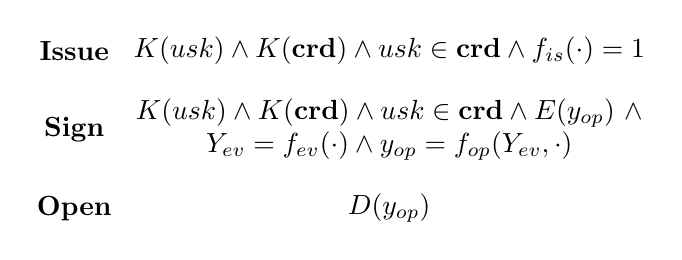
\begin{tikzpicture}

  \pgfdeclarelayer{bg}    % declare background layer
  \pgfsetlayers{bg,main}  % set the order of the layers (main is the standard layer)

  \node (issue) at (0.00,2.50) { \bf Issue };
  \node (sign) at (0.00,1.50) { \bf Sign };  
  \node (open) at (0.00,0.50) { \bf Open };

  \node (issue-uas) at (4.00,2.50)
  { $K(\usk) \land K(\scred) \land \usk \in \scred \land \fissue(\cdot) = 1$ };
  \node[align=center] (sign-uas) at (4.00,1.50)
  { $K(\usk) \land K(\scred) \land \usk \in \scred \land E(\yinsp)~\land$ \\
    $\Yeval = \feval(\cdot) \land \yinsp = \finsp(\Yeval,\cdot)$
  };
  \node (open-uas) at (4.00,0.50) { $D(\yinsp)$ };

  % \draw[draw=black,thick] (5.65,2.29) rectangle ++(1.43,0.44);
  % \draw[draw=black,dashed,thick] (1.80,1.09) rectangle ++(1.75,0.44);
  % \draw[draw=black,dotted,thick] (3.85,1.09) rectangle ++(2.30,0.44);
    
\end{tikzpicture}

%%% Local Variables:
%%% mode: latex
%%% TeX-master: t
%%% End:

  \caption{Summary of statements proved per operation in \UAS.
    $K(x)$ means proving knowledge of $x$; $E(y)$ means proving correct
    encryption of $y$; $D(z)$ means proving correct decryption of (an encryption
    of) $z$. Solid boxes span configurable statements that control issuance;
    dashed boxes span configurable statements that control utility at signing
    time; dotted boxes span configurable statements that control utility after
    signing time (accountability). Unboxed statements are fixed, and are thus
    common to all \UAS restrictions. $\usk \coloneqq$ user secret key; $\scred
    \coloneqq$ set of credentials.}
  \label{fig:proof-blocks-uas}
\end{figure}

From this generic construction, \CUASGen, one can already build known (and more
functionality-limited) schemes from what we call \emph{restrictions} of
\CUASGen simply by giving concrete definitions of \fissue, \feval, and \finsp.
Yet, the model remains the same, and we prove that if such restrictions of
\CUASGen are secure in the \UAS model, they lead to secure constructions for
the related primitives (GS variants, AC variants, etc). To define our generic
construction, we also specify concrete NP relations for the underlying NIZK
proofs for issuing, signing, and opening. Again with (unavoidable) minor variations
of these NP relations -- concretely to the one used for signing -- we show how
our \CUASGen variant can securely build ring signatures. That is, we prove that,
by simply tweaking a function, and treating all users as issuers, group
signatures an ring signatures are in essence the same thing.

We emphasize that, while -- already before \UAS -- it may have not seemed hard
to build either of these primitives from another, the core of our contribution
is that, with \UAS, one just needs to give concrete definitions of three
functions. Security of the final primitive then automatically follows from the
fact that it is a secure instantiation of an \UAS scheme. We believe that this
is a powerful notion, that may finally allow research lines (AC and GS) that
have followed different paths to benefit from the findings of each other.
\figref{fig:relations} graphically summarizes the relations we prove between
\UAS and other schemes -- although, of course, many more are probably
achievable.

\begin{figure}[ht!]
  \centering
  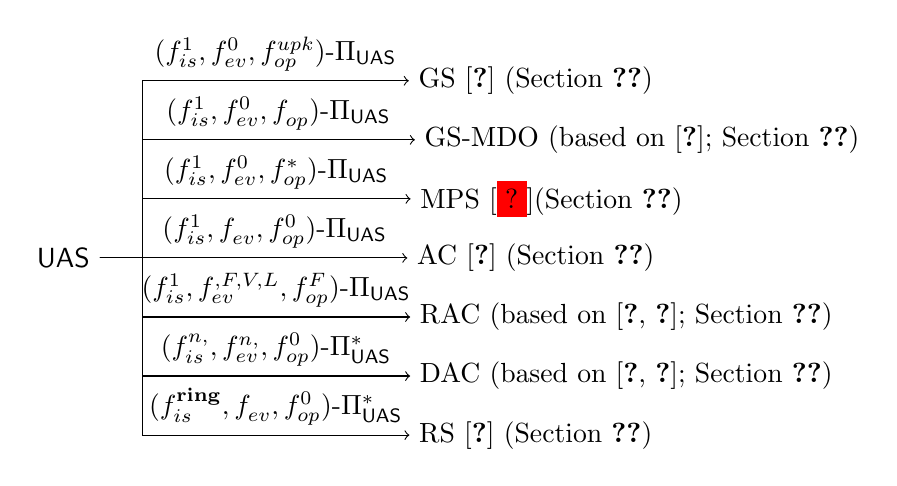
\begin{tikzpicture}

  \node (uas) at (0.00,2.25) { \bf \UAS };
  
  \node (gs) at (6.00,4.50) { GS \cite{bsz05} (\secref{xxx})};
  \node (gsmdo) at (7.35,3.75) { GS-MDO (based on \cite{seh+12}; \secref{xxx}) };
  \node (mps) at (6.20,3.00) { MPS \needcite (\secref{xxx}) };
  \node (ac) at (6.00,2.25) { AC \cite{fhs19} (\secref{xxx}) };
  \node (rac) at (7.15,1.50) { RAC (based on \cite{fhs19,cks10}; \secref{xxx}) };
  \node (dac) at (7.15,0.75) { DAC (based on \cite{fhs19,bcc+09}; \secref{xxx}) };
  \node (rs) at (6.00,0.00) { RS \cite{bkm06} (\secref{xxx}) };

  \draw[->] (uas) -- (1.00,2.25) -- (1.00,4.50) -- node[midway,above]
  {$(\fissue^1,\feval^0,\finsp^{\upk})$-\CUASGen} (gs);
  \draw[->] (uas) -- (1.00,2.25) -- (1.00,3.75) -- node[midway,above]
  {$(\fissue^1,\feval^0,\finsp^{\smsg})$-\CUASGen} (gsmdo);
  \draw[->] (uas) -- (1.00,2.25) -- (1.00,3.00) -- node[midway,above]
  {$(\fissue^1,\feval^0,\finsp^{\ast})$-\CUASGen} (mps);
  \draw[->] (uas) -- (1.00,2.25) -- node[midway,above]
  {$(\fissue^1,\feval^{\dattrs},\finsp^0)$-\CUASGen} (ac);
  \draw[->] (uas) -- (1.00,2.25) -- (1.00,1.50) -- node[midway,above]
  {$(\fissue^1,\feval^{\dattrs,F,V,L},\finsp^{F})$-\CUASGen} (rac);
  \draw[->] (uas) -- (1.00,2.25) -- (1.00,0.75) -- node[midway,above]
  {$(\fissue^{n,\dattrs},\feval^{n,\dattrs},\finsp^0)$-$\CUASGen^{\ast}$} (dac);
  \draw[->] (uas) -- (1.00,2.25) -- (1.00,0.00) -- node[midway,above]
  {$(\fissue^{\sring},\feval^{\attrs},\finsp^0)$-$\CUASGen^{\ast}$} (rs);
    
\end{tikzpicture}

%%% Local Variables:
%%% mode: latex
%%% TeX-master: t
%%% End:

  \caption{Summary of schemes that can be instantiated as restrictions of our
    generic construction, \CUASGen, and proved secure under our \UAS model.
    $\CUASGen^{\ast}$ denotes that minor changes to the basic construction
    beyond the concrete $(\fissue,\feval,\finsp)$-restrictions are needed.
    Between parenthesis we show the adopted reference model, and the section
    offering full detail.
  }
  \label{fig:relations}
\end{figure}

Before proceeding with our \UAS syntax and model in \secref{xxx}, generic
construction \CUASGen in \secref{xxx}, and relationships with other primitives
in \secref{xxx}, we give some preliminaries in \secref{xxx}. We conclude in
\secref{xxx}.

%%% Local Variables:
%%% mode: latex
%%% TeX-master: "uas-paper"
%%% End:

\section{Preliminaries}
\label{sec:preliminaries}

[3 pages max; 1.5 prelim, 1.5 GSAC]


%%% Local Variables:
%%% mode: latex
%%% TeX-master: "uas-paper"
%%% End:

\section{Formalizing \UAS}
\label{sec:formal-uas}

% [11 pages max]

Next we formalize our notion of Universal Anonymous Signatures
(\UAS). We define its syntax, model, and give a generic construction, which
we prove secure according to our model. 

The main contribution of this section is giving a simple syntax and model that
still allow spanning a wide variety of related schemes. We combine aspects of GS
and AC schemes, generalizing whenever possible. Like in ACs, there are multiple
issuers, and each user can get one or more credentials from any of them; and,
also, use more than one credential simultaneously to produce a signature. We
incorporate openers, as in GSs, but there is no tight relationship between
issuer and opener. As a consequence, signers (potentially along with verifiers)
may choose, on a per-signature basis, the policies governing the utility
information extractable from a signature. Finally, we incorporate functions that
allow tweaking the conditions checked at credential issuance and signature
generation times, including the information that an opener will be able to
extract from a signature. This flexibilizes the scheme even beyond the loose
relationship between issuer and opener.

\subsection{Syntax}
\label{ssec:syntax-uas}

An \UAS scheme is composed by the following algorithms:

\begin{description}
\item[$\Setup(\secpar) \rightarrow \parm$.] Given a security parameter \secpar,
  returns a global system parameter variable \parm. We assume that \parm are
  available to all the other functions, even if not explicitly listed in their
  input parameters.
\item[$\IKeyGen(\parm,\fissue) \rightarrow (\ipk,\isk)$.] Given \parm, and the
  function \fissue for checking that credential requestors meet the conditions
  to be issued a credential, an issuer runs \IKeyGen to generate its issuing key
  pair. 
\item[$\OKeyGen(\parm,\finsp) \rightarrow (\opk,\osk)$.] Given \parm, and the
  function \finsp, an opener runs \OKeyGen to generate its opening key pair.
  The function \finsp defines the type of utility that will be extractable from
  signatures.
\item[$\UKeyGen(\parm) \rightarrow \usk$.] Given \parm, returns a user's secret
  key.
\item[$\langle
  \Obtain(\usk,\ipk,\scred,\attrs),
  \Issue(\isk,\sipk,\attrs))
  \rangle \rightarrow \langle \cred/\bot,\utrans/\bot \rangle$.] %
  This interactive protocol lets a user with key \usk running the \Obtain
  process, receive a credential \cred from an issuer in the system, on attribute
  set $\attrs$. The user leverages a set of credentials \scred, each with a
  matching issuer key in \sipk (ommitted in \Obtain for readability). The user
  outputs the produced credential \cred, while the issuer outputs the protocol
  transcript \utrans for the produced credential.
\item[$\Sign(\usk,\opk,\scred,\msg,\feval) \rightarrow (\sig,\yeval)$.] %
  Upon receiving a user secret key \usk, opener public key \opk, a set of
  credentials \scred, a message \msg and evaluation function \feval, returns
  signature \sig, and a plaintext value \yeval. For readability, we assume
  that, for each $\cred \in \scred$, we can get the corresponding issuer public
  key \ipk; also, we use use \Sig to denote the tuple $(\sig,\yeval)$.
\item[$\Verify(\opk, \sipk,\Sig,\msg,\feval) \rightarrow 1/0$.]
  Checks whether $\Sig = (\sig,\yeval)$ is a valid signature
  over message \msg, from a user with credentials issued by issuers with public
  keys in \sipk, for evaluation function \feval and opener key \opk.
\item[$\Open(\osk,\sipk,\Sig,\msg,\feval) \rightarrow
  (\yinsp,\iproof)/\bot$.]
  Executed by the opener with private key \osk. Receives a signature $\Sig=
  (\sig,\yeval)$ over message \msg and evaluation function \feval,
  generated using credentials issued by the issuers with public keys in \sipk.
  If \Sig is valid, the function outputs a value $\yinsp$, and a proof of
  correct opening \iproof.
\item[$\Judge(\opk,\sipk,\yinsp,\iproof,\Sig,\msg,\feval) \rightarrow 1/0$.] %
  Checks if \iproof is a valid opening correctness proof for the value \yinsp,
  obtained by applying \Open to the the signature $\Sig = (\sig,\yeval)$
  over message \msg, and for evaluation function \feval. 
\end{description}

\paragraph{Issuance, evaluation, and opening functions.} %
We introduce three functions in our syntax and model. Through them,
it is possible to modulate the behaviour of the resulting instantiation, by
controling the conditions upon which a new credential can be issued, or the
information revealed at signing time, or after signing. In all cases, it is
the user who computes them, and has to prove correctness of such computation.
We give concrete examples in \secref{sec:relationships}, and define them next:

\begin{description}
\item[$\fissue: (\usk,\attrs_{\scred},\attrs)
  \rightarrow 0/1$.] Chosen by each issuer within a family of functions
  \famfissue, the issuance function defines the customized conditions required
  by the issuer to grant a credential over attributes \attrs, when requested by
  a user with secret key \usk, potentially leveraging a set of previously
  obtained credentials with attributes $\attrs_\scred$. \fissue returns $1$ to
  accept a request, $0$ to reject it.
\item[$\feval: (\usk,\attrs_{\scred},\msg)
  \rightarrow (\yeval^0,\yeval^1)$.] Signing evaluation functions, from a
  family of functions \famfeval, can be set on a per-signature basis. They
  receive the user secret key \usk, a set $\attrs_{\scred}$ of attributes in the
  credenetial used for signing, and message to be signed
  \msg. \feval outputs two values, $\yeval^0$ and $\yeval^1$, where the former
  is revealed in plaintext along with the signature, and $\yeval^1$ is
  encrypted. Both can be used to modulate the bevahiour of \finsp, and must
  belong in a well defined set \rngfeval. For readability, we write $\Yeval =
  (\yeval^0,\yeval^1)$.
\item[$\finsp: (\Yeval,\usk,\attrs_{\scred},\msg) \rightarrow \yinsp$.]
  Chosen by openers from a family of functions \famfinsp. The opening
  functions define what utility value, derived from the user's secret key,
  credentials used for signing, and signed message, should be extractable by an
  opener. Its behaviour can be modulated by \Yeval, and it outputs a value
  \yinsp, which must belong in a well defined set \rngfinsp.
\end{description}

\feval and \finsp may seem redundant. However, observe that the former is chosen
on a per-signature basis, probably after negotiation between signer and
verifier. As such, it governs the information revealed at signing time. On the
other hand, \finsp governs the information that may be revealed after signing.
Moreover, it is defined by openers, and even though signers and verifiers
may negotiate to use any opener for a given signature, it is not possible for
an opener to change the chosen function.

\begin{definition}{(\CUASGen restrictions)}
  \label{def:uas-restrictions}
  Let \CUASGen be a construction of an \UAS scheme, secure according to
  the model defined in \secref{ssec:model-uas}, and three functions $\fissue^a$,
  $\feval^b$, $\finsp^c$ compatible with the previous definitions. We say that
  \CUASGen, instantiated with $\fissue^a$, $\feval^b$, and $\finsp^c$, is a
  $(\fissue^a,\feval^b,\finsp^c)$-restriction of \CUASGen.
\end{definition}

% To summarize the previous, we depict in \figref{fig:uas-signature} the structure
% of an \UAS signature, including its main components and how they enable the
% previously stated generalization claims.

% \begin{figure}[ht!]
%   \centering
%   %\input{figures/uas-signature.tex}
%   \caption{Structure of an \UAS signature.}
%   \label{fig:uas-signature}
% \end{figure}

\subsection{Security Model}
\label{ssec:model-uas}

We define the security expected from an \UAS scheme using a game-based approach.
An \UAS scheme must ensure privacy at credential issuance, meaning that two
runs of the credential issuance protocol should not leak any information beyond
necessary about the user requesting the credential. Note that this is now
crucial for privacy since, as AC schemes, \UAS allows multiple credentials per
user -- thus, knowing what user is requesting which credential can lead to user
profiling. It must also ensure signature privacy, meaning that no information
can be learned by third parties from a signature, beyond what the user chooses
to reveal, and what may be extractable by the chosen opener. Issuance
unforgeability requires that \UAS schemes ensure that the claims used to support
a credential request cannot be falsified (issuance unforgeability). Similarly,
signature unforgeability requires that no adversary should be able to falsify
the correctness proofs for the claims included in the signatures. In both cases
(issuance and signature unforgeability), we require all credentials involved in
the corresponding process to be associated to a known user. Finally, \UAS
schemes inherit the useful non-frameability property of GS schemes where even
the issuer is corrupt. In this case, we can ensure that no honest user
can be framed with having created a signature that s/he did not create --
although the concept may get a bit blurred, as there is no traditional opening.
%
We describe next the global variables and oracles that we use in our modelling.

\paragraph{Global Variables.} %
Users are referred to with user identifiers, \uid; for credentials, we use \cid;
for issuers, \iid; and for openers, \oid. In all cases, we use bold font to
denote sets: e.g., \scid and \siid denote sets of credential and issuer
identifiers. All tables/sets are initialized as empty tables/sets.

\begin{description}
\item[$\mathsf{H}\lbrace\mathsf{U},\mathsf{I},\mathsf{O} \rbrace$.] Keep
  track of honest users/issuers/openers. They are sets of
  {\uid}s/{\iid}s/{\oid}s.
\item[$\mathsf{C}\lbrace\mathsf{U},\mathsf{I},\mathsf{O} \rbrace$.] Keep
  track of corrupt users/issuers/openers. They are sets of
  {\uid}s/{\iid}s/{\oid}s.    
\item[\UK.] \UK maintains user keys $\usk$. To refer to the key of a specific
  user, we use $\UK[\uid]$. 
\item[\IK, \PUBIK and \PRVIK.] \IK maintains issuer key pairs, where
  $\IK[\iid]$ refers to the key pair of the issuer with identifier \iid. We
  use \PUBIK to refer to the public component, which also includes the \fissue
  function; and \PRVIK refers to the private component of the key pair.
\item[\OK, \PUBOK, \PRVOK.] Same as \IK, but for opener key pairs. Instead
  of \fissue, \OK includes the \finsp function.
\item[\CRED.] Stores information related to credentials obtained by users in
  the system. Thus, it is indexable by \cid. More specifically, it stores
  tuples of the form $(\uid,\cred,\iid,\attrs,\scid,\siid)$, where \uid is the
  identity of the owner of the credential, \cred (when available) is the
  credential itself, \iid is the identifier of the credential issuer, \attrs
  are the attributes included in \cred, \scid are the identifiers of the
  credentials (if any) that \uid used to request \cred, and \siid the issuers
  of those credentials. For notational
  convenience, we may use $\CRED[\scid]$ to refer to $\CRED[\cid]$ for all
  $\cid \in \scid$. Also, when clear from context, we sometimes use
  $\CRED[\cid]$ (resp. $\CRED[\scid]$ to mean \cred (resp. \scred) in
  $\CRED[\cid] = (\cdot,\cred,\cdot,\cdot,\cdot)$ (resp. $\CRED[\scid]$).
\item[\CCRED.] Like \CRED, but keeps track of challenge credentials in the
  issuance anonymity game.
\item[\OWNR.] For notational convenience, when we write $\OWNR[\cid]$ we mean
  ``\uid such that $\CRED[\cid] = (\uid, \cdot, \cdot, \cdot, \cdot)$''.
\item[\ATTR.] For notational convenience, when we write $\ATTR[\cid]$ we mean
  ``\attrs such that $\CRED[\cid] = (\cdot, \cdot, \cdot, \attrs, \cdot)$''.
\item[\ISR.] For notational convenience, when we write $\ISR[\cid]$ we mean
  ``\iid such that $\CRED[\cid] = (\cdot, \iid, \cdot, \cdot, \cdot)$''.
\item[\SIG.] Maintains signatures generated via the \SIGN oracle. Entries of
  this table are $(\oid,\scid,\sig,\Yeval,\msg,\feval)$ tuples, where \oid is
  the opener, \scid is the set of credentials used for
  signing, \feval is the signing evaluation function, and \sig and \msg are the
  produced signature and signed message.
\item[\CSIG.] Maintains challenge signatures output to the adversary in the
  signature anonymity game, and is indexable by challenge signatures \csig.
  Each entry contains also $\cuid_b$ and $\cscid_b$, respectively the challenge
  user  and credential identifiers set used to produce \csig; as well as the
  corresponding challenge user and credential set indexed by the complementary
  $1-b$; the signed message \msg and signing evaluation function \feval, the
  result of \feval, \Yeval, and the opener identifier \oid.
\end{description}

\paragraph{Oracles.} %
In the game-based definitions of our \UAS model, we leverage the following
oracles, which are formally defined in \figref{fig:oracles1} and
\figref{fig:oracles2}. 

\begin{description}
\item[\IGEN.] Adds a new issuer to the game, generating its keypair and setting
  the associated issuance function.
\item[\OGEN.] Adds a new opener to the game, generating its key pair and
  setting the associated evaluation and inspection functions.
\item[\ICORR.] Corrupts an existing (and honest) issuer, by giving its secret
  key to the adversary.
\item[\OCORR.] Corrupts an existing (and honest) opener, by giving its secret
  key to the adversary.  
\item[\HUGEN.] Adds a new honest user to the game, by honestly generating
  the user's key pair.
\item[\CUGEN.] Adds a new corrupt user to the game or, if the specified
  user already exists and is honest, corrupts it, leaking its key and
  credentials.
\item[\RREG.] Reads the given transcript table entry.
\item[\WREG.] Sets a transcript table entry to the given value.
\item[\OBTISS.] Lets the adversary add a new honestly generated credential to
  the game, on behalf of an honest user.
\item[\OBTAIN.] Enables the adversary to play the role of a dishonest issuer, by
  letting it interact with honest users who want to receive credentials.
\item[\ISSUE.] Allows the adversary to play the role of dishonest users,
  requesting an honest issuer to produce credentials for them.
\item[\SIGN.] Lets the adversary get signatures from credentials belonging
  to honest users.
\item[\OPEN.] Given an honestly produced signature, outputs the result of the
  opening function, along with a correctness proof.
\item[\OBTCHALb.] Upon receiving a target credential identifier, two challenge
  users and credential sets, an honest issuer identifier, and a set of
  attributes, issues a credential for the challenge user and credential set
  defined by the bit $b$. 
\item[\CHALb.] Upon receiving two challenge users and credential sets, a common
  singing evaluation function and a message, returns a signature produced by one
  of these two user and credential sets, defined by the bit $b$.
\end{description}

{%\setlength\intextsep{\sep}
  \begin{figure*}[htp!]
    \centering
    \scalebox{0.9}{

      \begin{minipage}[t]{0.55\textwidth}

        \procedure{$\IGEN(\iid,\fissue)$}{%
          \pcif \iid \in \HI \lor \iid \in \CI: \pcreturn \bot \\
          \pcif \fissue \notin \famfissue: \pcreturn \bot \\
          (\ipk,\isk) \gets \IKeyGen(\parm) \\
          \IK[\iid] \gets ((\ipk,\fissue),\isk) \\
          \HI \gets \HI \cup \lbrace \iid \rbrace \\
          \pcreturn \ipk \\
        }

        \procedure{$\ICORR(\iid)$}{%
          \pcif \iid \in \CI \lor \iid \notin \HI: \pcreturn \bot \\
          \HI \gets \HI \setminus \lbrace \iid \rbrace \\
          \CI \gets \CI \cup \lbrace \iid \rbrace \\
          \pcreturn \isk \\
        }        

        \procedure{$\HUGEN(\uid)$}{%
          \pcif \uid \in \HU \lor \uid \in \CU: \pcreturn \bot \\
          \usk \gets \UKeyGen(\parm) \\
          \UK[\uid] \gets \usk;
          \HU \gets \HU \cup \lbrace  \uid \rbrace \\
          \pcreturn \top \\
        }

        \procedure{$\RREG(i)$}{%
          \pcreturn \trans[i]
        }        
        
      \end{minipage}
    }
    \scalebox{0.9}{
      
      \begin{minipage}[t]{.5\textwidth}

        \procedure{$\OGEN(\oid,\finsp)$}{%
          \pcif \oid \in \HO \lor \oid \in \CO: \pcreturn \bot \\
          \pcif \finsp \notin \famfinsp: \pcreturn \bot \\
          (\opk,\osk) \gets \OKeyGen(\parm) \\
          \OK[\oid] \gets ((\opk,\finsp),\osk) \\
          \HO \gets \HO \cup \lbrace \oid \rbrace \\
          \pcreturn \opk \\
        }

        \procedure{$\OCORR(\oid)$}{%
          \pcif \oid \in \CO \lor \oid \notin \HO: \pcreturn \bot \\
          \pcif \exists (\oid,\cdot,\cdot,\cdot,\cdot,
          \cdot,\cdot,\cdot,\cdot) \in \CSIG: \pcreturn \bot \\
          \HO \gets \HO \setminus \lbrace \oid \rbrace \\
          \CO \gets \CO \cup \lbrace \oid \rbrace \\
          \pcreturn \osk \\
        }        
        
        \procedure{$\CUGEN(\uid)$}{%          
          \pcif \uid \in \CU: \pcreturn \bot \\
          \CU \gets \CU \cup \lbrace \uid \rbrace \\          
          \pcif \uid \in \HU: \\
          \pcind \HU \gets \HU \setminus \lbrace \uid \rbrace; \\
          \pcind \pcreturn (\UK[\uid],\CRED[\uid]) \\
          \pcelse: \UK[\uid] = \bot \\          
          \pcreturn \top \\
        }

        \procedure{$\WREG(i,\rho)$}{%
          \trans[i] \gets \rho
        }        
        
      \end{minipage}
      
    }

    \caption{Detailed oracles available in our model (1/2). Oracles for
      generating key material for users, issuers, and openers.}
    \label{fig:oracles1}
  \end{figure*}
}

{%\setlength\intextsep{\sep}
  \begin{figure*}[htp!]
    \centering
    \scalebox{0.9}{

      \begin{minipage}[t]{0.55\textwidth}

        \procedure{$\OBTISS(\cid,\uid,\iid,\attrs,\scid)$}{%
          \pcif \uid \notin \HU: \pcreturn \bot \\
          \pcif \iid \notin \HI: \pcreturn \bot \\
          \pcif \exists \cid' \in \scid~\suchthat~\cid' \in \CCRED: \pcreturn \bot \\
          \pcif \CRED[\cid] \neq \bot \lor \CCRED[\cid] \neq \bot: \pcreturn \bot \\
          \langle \cred, \utrans \rangle \gets
          \langle \Obtain(\UK[\uid],\CRED[\scid],\attrs), \\
          \hspace*{60pt} \Issue(\PRVIK[\iid],\ISR[\scid],\attrs)
          \rangle \\
          \trans[\cid] \gets \utrans \\
          \CRED[\cid] \gets (\uid, \cred, \iid, \attrs, \scid, \siid) \\
          \pcreturn \top \\
        }

        \procedure{$\ISSUE(\cid,\uid,\iid,\attrs,\siid)$}{%
          \pcif \uid \notin \CU: \pcreturn \bot \\          
          \pcif \iid \notin \HI: \pcreturn \bot \\
          \pcif \CRED[\cid] \neq \bot \lor \CCRED[\cid] \neq \bot: \pcreturn \bot \\
          \langle \cdot, \utrans \rangle \gets
          \langle \adv, 
          \Issue(\PRVIK[\iid],\siid,\attrs) \rangle \\
          \trans[\cid] \gets \utrans \\
          \CRED[\cid] \gets (\uid, \cdot, \iid, \attrs, \cdot, \siid) \\
          \pcreturn \top \\          
        }

        \procedure{$\SIGN(\uid,\oid,\scid,\msg,\feval)$}{%
          \pcif \uid \notin \HU: \pcreturn \bot \\
          \pcif \exists \cid,\cid' \in \scid~\suchthat~\cid \in \CRED \land
          \cid' \in \CCRED: \\
          \pcind \pcreturn \bot \\
          \pcif \feval \notin \famfeval: \pcreturn \bot \\
          \Sig \gets \Sign(\UK[\uid],\PUBOK[\oid],\CRED[\scid],\msg,\feval) \\
          \Yeval=(\yeval^0,\yeval^1) \gets \feval(\UK[\uid],\CRED[\scid],\msg) \\
          \pcif \Yeval \notin \rngfeval: \pcreturn \bot \\
          \SIG[\uid] \gets \SIG[\uid] \cup
          \lbrace (\oid,\scid,\Sig,\Yeval,\msg,\feval) \rbrace \\
          \pcreturn \Sig \\
        }        

        \procedure{$\OPEN(\oid,\Sig,\msg)$}{%
          \textrm{Let}~\uid~\textrm{be s.t.}~(\oid,\scid,\Sig,\Yeval,\msg,\feval)
          \in \SIG[\uid] \\
          (\yinsp,\iproof) \gets
          \Open(\PRVOK[\oid],\PUBIK[\scid],\Sig,\msg,\feval) \\
          \pcif \CSIG[\Sig] \neq \bot: \\
          \pcind \textrm{Parse $\CSIG[\Sig]$ as $(\oid,\cuid_b,\scid_b,
            \Yeval,\msg,\feval$} \\          
          \hspace*{83pt}\cuid_{1-b},\cSig_{1-b},\scid_{1-b},
          \TYeval) \\
          \pcind (\tyinsp,\tiproof) \gets
          \Open(\PRVOK[\oid],\IK[\siid],\\
          \hspace*{107pt} \cSig_{1-b},\msg,\feval) \\
          \pcind \pcif \tyinsp \neq \yinsp: \pcreturn \bot \\
          \pcreturn (\yinsp,\iproof)
        }
        
      \end{minipage}
    }
    \scalebox{0.9}{
      
      \begin{minipage}[t]{.5\textwidth}

        \procedure{$\OBTAIN(\cid,\uid,\iid,\attrs,\scid)$}{%
          \pcif \uid \notin \HU: \pcreturn \bot \\
          \pcif \iid \notin \CI: \pcreturn \bot \\
          \pcif \exists \cid' \in \scid~\suchthat~\cid' \in \CCRED: \pcreturn \bot \\
          \pcif \CRED[\cid] \neq \bot \lor \CCRED[\cid] \neq \bot: \pcreturn \bot \\
          \langle \cred, \cdot \rangle \gets
          \langle \Obtain(\UK[\uid],\PUBIK[\iid],\CRED[\scid],\attrs),\adv \rangle \\
          \CRED[\cid] \gets (\uid, \cred, \iid, \attrs, \scid, \siid) \\
          \pcreturn \top \\
        }

        \procedure{$\OBTCHALb(\cid,\cuid_{0,1},\iid,\attrs,\cscid_{0,1})$}{%
          \pcif \cuid_0 \notin \HU \lor \cuid_1 \notin \HU: \pcreturn \bot \\
          \pcif \iid \notin \CI: \pcreturn \bot \\
          \pcif \CRED[\cid] \neq \bot: \pcreturn \bot \\
          \pcif \pcfor d \in \bin,~ \exists \cid' \in \cscid_d~\suchthat~\cid'
          \in \CRED: \\
          \pcind \pcreturn \bot \\
          \pcif \PUBIK[\cscid_0] \neq \PUBIK[\cscid_1]: \pcreturn \bot \\
          \textrm{Parse}~\PUBIK[\iid]~\textrm{as}~((\cdot,\fissue),\cdot) \\
          \pcif \fissue(\UK[\cuid_0],\cscid_0,\attrs) \neq
          \fissue(\UK[\cuid_1],\cscid_1,\attrs) \\
          \langle \cred, \cdot \rangle \gets
          \langle \Obtain(\UK[\cuid_b],\PUBIK[\iid],\CRED[\cscid_b],\attrs),\adv \rangle \\
          \CCRED[\cid] \gets (\cuid_b, \cred, \iid, \attrs, \cscid_b, \siid) \\
          \pcreturn \top \\
        }

        \procedure{$\CHALb(\cuid_{0,1},\oid,\cscid_{0,1},\msg,\feval)$}{%
          \pcif \cuid_0 \notin \HU \lor \cuid_1 \notin \HU: \pcreturn \bot \\
          \pcif \pcfor d \in \bin~ \exists \cid,\cid' \in \scid_d~\suchthat \\
          \pcind \cid \in \CRED \land \cid' \in \CCRED: \pcreturn \bot \\
          \pcif \oid \in \CO: \pcreturn \bot \\
          \pcif \feval \notin \famfeval: \pcreturn \bot \\          
          \Yeval = (\yeval^0,\yeval^1) \gets \feval(\UK[\cuid_0],\CRED[\cscid_0],
          \msg) \\
          \TYeval = (\tyeval^0,\tyeval^1) \gets
          \feval(\UK[\cuid_1],\CRED[\cscid_1],\msg) \\
          \pcif \yeval^0 \neq \tyeval^0: \pcreturn \bot \\
          \pcif \Yeval \notin \rngfeval \lor \TYeval \notin \rngfeval:
          \pcreturn \bot \\
          \pcif \PUBIK[\cscid_0] \neq \PUBIK[\cscid_1]: \pcreturn \bot \\
          \cSig_b \gets \Sign(\UK[\cuid_b],\PUBOK[\oid], \\
          \hspace*{71pt}\CRED[\cscid_b],\msg,\feval) \\
          \cSig_{1-b} \gets \Sign(\UK[\cuid_{1-b}],\PUBOK[\oid], \\
          \hspace*{80pt}\CRED[\cscid_{1-b}],\msg,\feval) \\          
          \CSIG[\cSig_b] \gets 
          \lbrace (\oid,\cuid_b,\cscid_b,\Yeval,\msg,\feval,\\
          \hspace*{74pt}\cuid_{1-b},\cSig_{1-b},\cscid_{1-b},\TYeval)\rbrace \\
          \pcreturn \cSig_b
        }
        
      \end{minipage}
      
    }

    \caption{Detailed oracles available in our model (2/2). Oracles for
      obtaining credentials, signatures, and processing them.}
    \label{fig:oracles2}
  \end{figure*}
}

\paragraph{Helper functions \SimSetup, \ExtractIssue, \ExtractSign,
  \IdentifyCred, and \IdentifySig.} We assume the existence of these helper
functions. They are not functions available in the actual scheme, but rather to
the challenger in the experiments we use to formalize security of \UAS schemes.
Consequently, while we introduce them here and specify some conditions they need
to meet, their full definition is dependent on the construction. We fully define
them for our generic construction \CUASGen in \appref{app:uas-proofs}. Similar
techniques have been used before to prove security in privacy-preserving schemes
with some sort of accountability, but that do not offer conventional opening as
vanilla group signatures. For instance, see related works on DAA
\cite{bfg+11,cdl16} and group signature variants \cite{dl21,fgl21,gl19,lnpy21}.
More concretely, these functions are as follows:

\begin{description}
\item[$\SimSetup(1^\secpar) \rightarrow (\parm,\trap)$.] Given a security
  parameter, outputs global (simulated) parameters \parm whose distribution is
  indistinguishable to that produced by the \Setup algorithm, as well as a
  trapdoor \trap.
\item[$\ExtractIssue(\trap,\utrans) \rightarrow (\usk,\attrs_{\scred},\scred)$.]
  Receives trapdoor \trap and an $\langle \Obtain, \Issue \rangle$ transcript,
  and returns the credentials (if any) and their attributes involved in the
  request. It needs an honest issuer as, otherwise, the transcripts won't be
  available. 
\item[$\ExtractSign(\trap,\oid,\siid,\Sig,\msg,\feval) \rightarrow (\usk,
  \scred,\attrs_{\scred},\yeval^1,\yinsp)$.] Receives a trapdoor \trap, a
  signature \Sig,
  as well as the opener identifier \oid, and the identifiers of all issuers of
  the credentials used to produce the signature over \msg, and for \feval.
  It outputs the user secret key and credentials (with their attributes) used to
  generate the signature, and the $\yeval^1$ and \yinsp values.
\item[$\IdentifyCred(\trap,\usk,\attrs_{\cred},\cred,\ipk)$.] Returns $1$ if
  \cred has been issued over attributes $\attrs_{\cred}$ and for a user with
  secret key \usk, by honest issuer with public key \ipk. Otherwise, it returns
  $0$.

  The \IdentifyCred function defined by \UAS constructions must satisfy that
  for any \cred obtained as the result of an $\langle \Obtain,\Issue \rangle$
  interaction with an honest issuer, there exists \emph{exactly one} set of
  $(\usk,\attrs_{\cred})$ such that \IdentifyCred equals $1$.
  %In order to be meaningful, this requires that,
  %for every $(\attrs_{\cred},\cred)$ pair, there is at most one \usk that makes
  \IdentifyCred return $1$.
\item[$\IdentifySig(\trap,\usk,\scred,\Sig)$.] Returns $1$ is $(\usk,\scred)$
  are the secret key and credential set used to produce \Sig, otherwise, returns
  $0$.

  The \IdentifySig function defined by \UAS constructions must satisfy that, for
  signatures accepted by \Verify, there must exist \emph{exactly one} $(\usk,
  \scred)$ combination that makes \IdentifySig return $1$.
  % . This is trivial for honest users, for which there must be a one-to-one
  % relationship between {\uid}s and {\usk}s. For corrupt users, \IdentifyUK has
  % to iterate through the $\langle\Obtain,\Issue\rangle$ transcripts associated
  % to \uid, extract the used secret key, and check if there is a match. In the
  % latter case, there is no guarantee of getting a one-to-one relationship
  % between \usk and \uid. Also, when used for corrupt users, this can only be
  % used when the issuer is honest, as transcripts are needed. 
\end{description}

% Note that, for all the helper functions, in the case of credentials, transcripts,
% and signatures by honest users, it is enough to have access to the corresponding
% state information (described below) maintained by the challenger in our
% experiments. For credentials and join transcripts of corrupt users, or
% dishonestly produced signatures, we do need to perform actual extraction.
% Certainly, the challenger
% needs special knowledge/power such as decryption trapdoors, the ability to
% rewind the game, or program random oracles. The approach needs thus to depend on
% the concrete construction. \jdv{Although, for the case of \ExtractIssue and
%   \IdentifyUK, online extractability (or alternative requirements, such as
%   non-parallel or logarithmic number of joins) is necessary.}

\paragraph{Correctness.} %
Correctness of \UAS schemes is formalized through the experiment in
\figref{fig:exp-uas-corr}. It states that a signature over any arbitrary message
and valid function \feval, produced honestly leveraging credential set \scid,
owned by user \uid, is accepted by \Verify. Moreover, all the credentials in
\scid meet the conditions set by the corresponding \fissue defined by the issuer
which issued each credential. Similarly, the output of \feval matches the
value produced by \Sign alongside with \sig; and the value produced by \Open
is accepted by \Judge, and matches the output of applying \finsp on \Yeval, the
credentials, user key, and message.

\begin{definition}{(Correctness of \UAS)}
  \label{def:correctness-uas}
  An \UAS scheme is correct if, for any p.p.t. adversary $\adv$,
  $\ExpCorrect(1^\secpar)$ outputs 1 with negligible probability.
\end{definition}

\begin{figure}[htp!]
  \procedure[linenumbering]{$\ExpCorrect(1^\secpar)$}{%
    \parm \gets \Setup(1^\secpar) \\
    (\uid,\oid,\scid,\msg,\feval)
    \gets \adv^{\IGEN,\OGEN,\HUGEN,\OBTISS,\RREG}(\parm) \\
    \pcif \feval \notin \famfeval: \pcreturn 0 \\
    \pcif \OWNR[\scid] \neq \uid: \pcreturn 0 \\
    (\Sig = (\sig,\yeval)) \gets \Sign(\UK[\uid],\PUBOK[\oid],\scid,\msg,
    \feval) \\
    \pcif \Verify(\PUBOK[\oid],\PUBIK[\scid],\Sig,\msg,\feval) = 0: \pcreturn 1 \\
    \pcfor \cid \in \scid \pcdo: \\
    \pcind \textrm{Let}~\scred^{\cid}~\textrm{be the credentials used to obtain}
    ~\cid;~\textrm{Parse}~\PUBIK[\ISR[\cid]]~\textrm{as}~((\cdot,\fissue^{\cid}),\cdot)\\
    \pcind \pcif \fissue^{\cid}(\UK[\uid],\scred^{\cid},\ATTR[\cid]) = 0: \pcreturn 1 \\
    (\yeval^0,\yeval^1) \gets \feval(\UK[\uid],\CRED[\scid],\msg) \\
    \pcif \yeval^0 \neq \yeval: \pcreturn 1 \\
    (\yinsp,\iproof) \gets \Open(\PRVOK[\gid],\PUBIK[\scid],\Sig,\msg,\feval) \\
    \pcif \Judge(\PUBOK[\oid],\PUBIK[\scid],\yinsp,\iproof,\Sig,\msg,\feval)
    = 0~\lor \\
    \pcind \yinsp \neq \finsp^\gid((\yeval,\yeval^1),\UK[\uid],\CRED[\scid],\msg)): \\
    \pcind \pcreturn 1 \\
    \pcreturn 0
  }  
  \caption{Correctness experiment for \UAS schemes.}
  \label{fig:exp-uas-corr}
\end{figure}

\subsubsection{Security Properties}
\label{sssec:security}

Security of an \UAS scheme is defined in terms of anonymity, unforgeability and
non-frameability. Where the first two have variants covering issuance and
signatures \todo{argue why issuance non-frameability does not make sense}.
%
However, as stated, we make use of some helper functions: \ExtractIssue and
\ExtractSign, which let us recover the witnesses used to produce a credential
or a signautre; and \IdentifyCred, and \IdentifySig, which associate credentials
and signatures to user identifiers \uid. Both types of functions have been used
before. For instance, the extraction-type are used in \cite{lnpy21,nps22}, and
functions of the identify-type are used in \cite{bfg+11,cdl16,gl19,dl21,fgl21}.
\todo{Re-write after done.} Indeed, it seems hard to avoid resorting to these
techniques when there is no traditional notion of opening.

\paragraph{Extractability.} %
We require that the witnesses used to produce each credential and signature can
be extracted from the corresponding \utrans and signature, respectively.
Furthermore, in order for our generalized notion of utility to have meaning, it
is required that, whenever a credential is issued by an honest issuer, or a
signature is accepted by \Verify, the extracted values produce the same value as
the chosen \fissue, \feval and \finsp functions. We capture this in the
\ExpExtractIssue and \ExpExtractSign games, which are crucial in the
unforgeability and non-frameability requirements.

\begin{figure*}[htp!]
  \centering
  \scalebox{0.9}{
    \begin{minipage}[t]{0.6\textwidth}
      \procedure[linenumbering]{$\ExpExtractIssue(1^\secpar)$}{%
        (\parm, \trap) \gets  \SimSetup(1^\secpar) \\
        \cid \gets \adv^{\todo{\OExtIss}}(\parm) \\
        (\usk,\scred,\attrs_{\scred}) \gets \ExtractIssue(\trap,\trans[\cid]) \\
        \pcif \fissue(\usk,\scred,\ATTR[\cid]) = 0: \pcreturn 1 \\
        \pcreturn 0
      }
    \end{minipage}
    \vspace*{0.5em}
    
    \begin{minipage}[t]{0.5\textwidth}
      \procedure[linenumbering]{$\ExpExtractSign(1^\secpar)$}{%
        (\parm, \trap) \gets \SimSetup(1^\secpar) \\
	(\oid,\siid,\Sig=(\sig,\yeval),\msg,\feval) \gets
        \adv^{\todo{\OExtSig}}(\parm) \\
	\pcif \Verify(\oid,\siid,\Sig,\msg,\feval) = 0: \pcreturn 0 \\
	(\usk,\scred,\attrs_{\scred},\yeval^1,\yinsp) \gets        
        \ExtractSign(\trap,\oid,\siid,\Sig,\msg,\feval) \\
        (\yeval^0,\yeval^1) \gets \feval(\usk,\scred,\msg) \\
        \pcif \yeval \neq \yeval^0 \lor \yeval^1 \neq \tyeval^1:
        \pcreturn 1 \\
        \pcif \finsp((\yeval^0,\yeval^1),\usk,\scred,\msg) \neq \yinsp:
        \pcreturn 1 \\
	\pcreturn 0
      }
    \end{minipage}
  }
  \caption{Extractability experiments for \UAS schemes.}
  \label{fig:exp-uas-extract}
\end{figure*}

\paragraph{Identifiability.} %
On their own, the extractability properties only ensure that the produced
credentials and signatures have been produced by leveraging knowledge of some
witnesses. However, they do not establish any relationship between those
witnesses and the identity of their owner(s). While the way in which witnesses
are associated to user identifiers\footnote{We avoid the term \emph{user
    identity}, as that is very context-specific.} is dependent on the
construction, we impose some constraints that all schemes need to satisfy.
Namely, it must be possible to associate any credential (obtained from an honest
issuer), or any signature accepted by \Verify, to exactly one user identifier.

\begin{figure*}[htp!]
  \centering
  \scalebox{0.9}{
    \begin{minipage}[t]{0.6\textwidth}
      \procedure[linenumbering]{$\ExpIdentifyCred(1^\secpar)$}{%
        (\parm, \trap) \gets  \SimSetup(1^\secpar) \\
        \cid \gets \adv^{\todo{\OIdCred}}(\parm) \\
        (\usk,\scred,\attrs_{\scred}) \gets \ExtractIssue(\trap,\trans[\cid]) \\
        \suid \gets \IdentifyCred(\trap,\usk,\scred,\attrs_{\scred},\ipk_{\cred}) \\
        \pcif |\suid| \neq 1: \pcreturn 1 \\
        \pcreturn 0
      }
    \end{minipage}
    \vspace*{0.5em}
    
    \begin{minipage}[t]{0.5\textwidth}
      \procedure[linenumbering]{$\ExpIdentifySign(1^\secpar)$}{%
        (\parm, \trap) \gets \SimSetup(1^\secpar) \\
	(\oid,\siid,\Sig,\msg,\feval) \gets \adv^{\todo{\OIdSig}}(\parm) \\
	\pcif \Verify(\oid,\siid,\Sig,\msg,\feval) = 0: \pcreturn 0 \\
	(\usk,\scred,\attrs_{\scred},\yeval^1,\yinsp) \gets
        \ExtractSign(\trap,\oid,\siid,\Sig,\msg,\feval) \\
	\suid \gets \IdentifySig(\trap,\usk,\scred,\Sig) \\
	\pcif |\suid| \neq 1: \pcreturn 1 \\
	\pcreturn 0
      }
    \end{minipage}
  }
  \caption{Identifiability experiments for \UAS schemes.}
  \label{fig:exp-uas-identify}
\end{figure*}

\begin{definition}{(Identifiable credentials in \UAS)}
  \label{def:identify-cred-uas}  
  We define the advantage \AdvIdCred of $\adv$ against \ExpIdentifyCred as
  $\AdvIdCred=|\Pr\lbrack\ExpIdentifyCred(1^\secpar)=1\rbrack-
  \Pr\lbrack\ExpIdentifyCred(1^\secpar)=1\rbrack|$.
  %
  An \UAS scheme satisfies identifiable credentials if, for any p.p.t. adversary
  $\adv$, \AdvIdentifyCred is a negligible function of $1^\secpar$.
\end{definition}

\begin{definition}{(Identifiable signatures in \UAS)}
  \label{def:identify-sig-uas}  
  We define the advantage \AdvIdSig of $\adv$ against \ExpIdentifySign as
  $\AdvIdSig=|\Pr\lbrack\ExpIdentifySign(1^\secpar)=1\rbrack-
  \Pr\lbrack\ExpIdentifySign(1^\secpar)=1\rbrack|$.
  %
  An \UAS scheme satisfies identifiable signature if, for any p.p.t. adversary
  $\adv$, \AdvIdSig is a negligible function of $1^\secpar$.
\end{definition}

\paragraph{Anonymity.} %
Users may see their privacy compromised through their interactions with issuers
to request a credential, or via the signatures they produce. Thus, we define two
games to define the privacy expected in those situations.

The issuance anonymity game captures that, given polymomially many
credential issuance interactions, the adversary gains no information about the
user(s) behind them. For this, we allow the adversary to control targetted
issuers and openers (although it may also add honest ones), and add honest and
corrupt users. The adversary can also obtain credentials, produce signatures,
and open them. We need to make some limitations to prevent trivial wins: first,
when querying the oracle for obtaining a challenge credential out of two
possible user-credential set pairs, the issuance protocol must either succeed or
fail for both; also, the adversary can open signatures produced with credential
sets containing challenge credentials $\cred_b$, only if the output of \Open is
the same as with the complementary $\cred_{1-b}$ (note that any other signature
can be open).
Intuitively, if the adversary cannot distinguish arbitrary runs with all oracles
(provided the previous constraint) when he gets challenge credentials $\cred_b$
from runs with credentials $\cred_{1-b}$, then the issuance protocol is
privacy-preserving.

The signature anonymity game is similar to the traditional one in GS schemes.
It captures that the signatures produced by system users do not leak information
about their identity beyond what is already revealed via $\yeval^0$ and what
may be revealed via \yinsp. Concretely, the adversary can interact with oracles
as in the issuance anonymity game, except that instead of obtaining challenge
credentials, it obtains challenge signatures. These signatures must have been
produced via the \CHALb oracle, which ensures that the $\yeval^0$ value is the
same for both input sets -- otherwise, rejects creating the signature. We also
allow opening signatures; even challenge $\cSig_b$ signatures, as long as the
\yinsp value of the counterpart $\cSig_{1-b}$ is the same. Note that this is
stronger than the traditional CCA-like security of group signatures, where no
challenge signature can be open.

The formal specification of the anonymity games is given in
\figref{fig:exp-uas-anonb}, where
$\OIssAnon \gets (\lbrace\HU,\CU\rbrace\GEN,\lbrace\II,\OO\rbrace\GEN,\lbrace\II,
\OO\rbrace\CORR,\OBTAIN,\WREG,\SIGN,\OPEN,\OBTCHALb)$, and $\OSigAnon
\gets (\lbrace\HU,\CU\rbrace\GEN,\lbrace\II,\OO\rbrace\GEN,\lbrace\II,\OO\rbrace
\CORR,\OBTAIN,\WREG,\SIGN,\OPEN,\CHALb)$.

\begin{figure*}[htp!]
  \centering
  \scalebox{0.9}{
    \begin{minipage}[t]{0.5\textwidth}
      \procedure[linenumbering]{$\ExpIssAnonb(1^\secpar)$}{%
        (\parm,\trap) \gets \SimSetup(1^\secpar) \\
        b^* \gets \adv^{\OIssAnon} (\parm) \\
        \pcreturn b^*
      }
    \end{minipage}
    
    \begin{minipage}[t]{0.5\textwidth}
      \procedure[linenumbering]{$\ExpSigAnonb(1^\secpar)$}{%
        (\parm,\trap) \gets \SimSetup(1^\secpar) \\
        b^* \gets \adv^{\OSigAnon} (\parm) \\
        \pcreturn b^*
      }
    \end{minipage}
  }
  \caption{Issuance and signature anonymity experiments for \UAS schemes.}
  \label{fig:exp-uas-anonb}
\end{figure*}

\begin{definition}{(Issuance anonymity in \UAS)}
  \label{def:issue-anonymity-uas}  
  We define the advantage \AdvIssAnon of $\adv$ against \ExpIssAnonb as
  $\AdvIssAnon=|\Pr\lbrack\ExpIssAnono(1^\secpar)=1\rbrack-
  \Pr\lbrack\ExpIssAnonz(1^\secpar)=1\rbrack|$.
  %
  An \UAS scheme satisfies issuance anonymity if, for any p.p.t. adversary
  $\adv$, \AdvIssAnon is a negligible function of $1^\secpar$.
\end{definition}

\begin{definition}{(Signature anonymity in \UAS)}
  \label{def:sign-anonymity-uas}  
  We define the advantage \AdvSigAnon of $\adv$ against \ExpSigAnonb as
  $\AdvSigAnon=|\Pr\lbrack\ExpSigAnono(1^\secpar)=1\rbrack-
  \Pr\lbrack\ExpSigAnonz(1^\secpar)=1\rbrack|$.
  %
  An \UAS scheme satisfies signature anonymity if, for any p.p.t. adversary
  $\adv$, \AdvSigAnon is a negligible function of $1^\secpar$.
\end{definition}

\paragraph{On the generality of anonymity in \UAS schemes.} %
From the point of view of the achieved privacy, depending on how one defines
\fissue, \feval and \finsp, it is easy to see that the resulting scheme would
have different privacy level. For instance, a scheme that has very granular
\feval outputs barely provides privacy. Or a scheme for which most signatures
include the same \finsp value has less accountability, but higher privacy.
%
This is a natural consequence of the fact that, with different choices of those
functions, one can mimic the behaviour of (more restricted) schemes. For
instance, by setting \finsp to output the signer's public key, and \feval to
output nothing, one gets the same anonymity as in vanilla group signatures
(concretely, no challenge signature can be opened). Or, if \feval outputs any
arbitrary subset of the attributes in the used credential(s), and \finsp outputs
any constant value, then we get the same anonymity as in conventional selective
disclosure anonymous credential schemes, where any pair of users with different
subset of revealed attributes are clearly distinguishable. The impact of \fissue
is somehow orthogonal to the previous, but can be seen as a kind of equivalent
to \feval, at issuance time.
%
Importantly, note that the model is agnostic to the concrete instantiation of
these functions, and just cares about whether their outputs are equal or not,
in order to avoid trivial wins by the adversary.

\paragraph{Unforgeability.} \UAS inherits from AC and GS schemes two different
notions of unforgeability: from AC schemes, the notion that no adversary can
prove claims unless it owns credentials with the proper attributes; from GS
schemes, that only credential owners can produce valid signatures. \UAS also
has verifiable openings as some group signature schemes, which sits somewhere
in between, and we must ensure that the values output by \Open are correct and
trace back to a user with consistent credentials. All the previous is captured
by a signature unforgeability property. We define this by allowing the adversary
to call any oracle, except the one for corrupting issuers. The adversary wins if
it produces a valid signature over some message that: (1), opens to a wrong
value, or to a value that cannot be processed by \Judge; (2), is not consistent
with the expected \Yeval value; or (3), cannot be associated to known
credentials owned by a known user.

Again, since \UAS schemes (may) require proving claims at issuance time, we
need to ensure that those claims cannot be forged by an adversary without the
proper attributes. In this case, since we (need to) assume trusted issuers, we
can condition on having the $\langle \Obtain,\Issue \rangle$ transcripts
available for analysis. Thus, the adversary -- with access to the same oracles
as above -- is challenged to output a credential identifier for a credential
that exists in \CRED and (1), the conditions required by \fissue were not
satisfied, or some of the credentials used to support the request does not
belong to the requesting user; or (2) all credentials used to support the
request are bound to the same secret key, but that secret key does not belong
to any known user. The issuance unforgeability notion formalizes this.

For both \ExpForgeIssue (in \figref{fig:exp-uas-unfor-issue}) and \ExpForgeSign
(in \figref{fig:exp-uas-unfor-sign}), the adversary is given access to the
oracle set $\Oforgeissue = \Oforgesign \gets \lbrace\HU,\CU\rbrace\GEN,\IGEN,
\OGEN,\OCORR,\OBTISS,\ISSUE,\RREG,\SIGN,\OPEN$.

\begin{figure}[htp!]
    \procedure[linenumbering]{$\ExpForgeIssue(1^\secpar)$}{%
      (\parm,\trap) \gets \SimSetup(1^\secpar) \\
      \cid \gets \adv^{\Oforgeissue}(\parm) \\
      \pcif \trans[\cid] = \bot \lor \CRED[\cid] = \bot: \pcreturn 0 \\
      \textrm{Parse}~\CRED[\cid]~\textrm{as}~(\cdot,\cdot,\iid,\cdot,\cdot);~
      \IK[\iid]~\textrm{as}~((\ipk,\fissue),\cdot) \\
      (\usk,\scred,\attrs_{\scred}) \gets \ExtractIssue(\trap,\trans[\cid]) \\
      \pcif \fissue(\usk,\scred,\ATTR[\cid]) = 0 \lor
      \exists \cred \in \scred~\suchthat~\IdentifyCred(\trap,\usk,
      \attrs_{\cred},\cred,\ipk) = 0: \\
      \pcind \pcreturn 1 \\
      \pcreturn 0
    }
  \caption{Experiment for unforgeability of credential issuance in \UAS schemes.}
  \label{fig:exp-uas-unfor-issue}
\end{figure}    

\begin{figure}[htp!]
    \procedure[linenumbering]{$\ExpForgeSign(1^\secpar)$}{%
      (\parm,\trap) \gets \Setup(1^\secpar) \\
      (\oid,\siid,\Sig=(\sig,\yeval),\msg,\feval) \gets \adv^{\Oforgesign}(\parm) \\
      \pcif \exists \uid~\suchthat~(\cdot,\cdot,\Sig,\cdot,\msg,\feval) \in
      \SIG[\uid]: \pcreturn 0 \\
      \pcif \Verify(\PUBOK[\oid],\PUBIK[\siid],\Sig,\msg,\feval) = 0:
      \pcreturn 0 \\
      (\yinsp,\iproof) \gets \Open(\PRVOK[\oid],\siid,\Sig,\msg) \\
      \pcif \Judge(\PUBOK[\oid],\PUBIK[\siid],\yinsp,\iproof,\Sig,\msg,\feval)
      = 0: \pcreturn 1 \\
      (\usk,\scred,\attrs_{\scred},\tyeval^1,\yinsp',r) \gets
      \ExtractSign(\trap,\oid,\siid,\Sig,\msg,\feval) \\
      \Yeval=(\yeval^0,\yeval^1) \gets \feval(\usk,\scred,\msg) \\
      \pcif \yeval \neq \yeval^0 \lor \yeval^1 \neq \tyeval^1:
      \pcreturn 1 \\
      \pcif \finsp((\yeval^0,\yeval^1),\usk,\scred,\msg) \neq \yinsp:
      \pcreturn 1 \\
      \pcif \exists \cred \in \scred~\suchthat~
      \IdentifyCred(\tau,\usk,\attrs_{\cred},\cred,\ipk_{\cred}) = 0:
      \pcreturn 1 \\
      \pcif \nexists \uid~\suchthat~\IdentifySig(\trap,\usk,\scred,\Sig) = 1:
      \pcreturn 1 \pccomment{\todo{\uid-\usk}} \\
      \pcreturn 0
    }
  \caption{Experiment for unforgeability of signatures in \UAS schemes.}
  \label{fig:exp-uas-unfor-sign}
\end{figure}

\begin{definition}{(Unforgeable issuance of \UAS)}
  \label{def:issue-forge-uas}  
  We define the advantage \AdvForgeIssue of $\adv$ against \ExpForgeIssue as
  $\AdvForgeIssue=\Pr\lbrack\ExpForgeIssue(1^\secpar)=1\rbrack$.
  %
  A \UAS scheme has unforgeable issuance if, for any p.p.t. adversary $\adv$,
  \AdvForgeIssue is a negligible function of $1^\secpar$.
\end{definition}

\begin{definition}{(Unforgeable signing of \UAS)}
  \label{def:sign-forge-uas}  
  We define the advantage \AdvForgeSign of $\adv$ against \ExpForgeSign as
  $\AdvForgeSign=\Pr\lbrack\ExpForgeSign(1^\secpar)=1\rbrack$.
  %
  A \UAS scheme has unforgeable signing if, for any p.p.t. adversary $\adv$,
  \AdvForgeSign is a negligible function of $1^\secpar$.
\end{definition}

For short, we say that an \UAS scheme that has both unforgeable issuance and
signing, is an unforgeable \UAS scheme.

\paragraph{On the generality of unforgeability in \UAS schemes.} %
Regarding the information revealed at signature time ($\yeval^0$), \UAS's
unforgeability notion is equivalent to that of known AC schemes. It is the
generalization of the information output at opening time ($\yinsp$), only
present up to know in MPS \needcite what makes the notion of unforgeability more
subtle. The fact that multiple users may produce signatures opening to the same
value necessarily forces to generalize what is a forgery -- and, certainly,
resorting to extraction-based techniques seems unavoidable.

As for anonymity, note that by tweaking the \fissue, \feval and \finsp
functions, one can easily mimic behaviour of more restricted schemes. For
instance, \feval, along with the $\yeval^0$ output, allows revealing
authenticated attribute-related information alongside the signatures, as in AC
schemes. Or, with \fissue, rules for delegation can be easily encoded, leading
to delegatable schemes.

\paragraph{Non-frameability.} %
The notion of non-frameability in \UAS schemes is unavoidably more subtle than
in group signatures. To see this, we note that, by allowing arbitrary
evaluation and open functions to be used, it can be perfectly valid to
have a signature produced by a corrupted user output the same \yeval or \yinsp
values than the ones output when evaluating or opening a signature by an honest
user.
%
More generally, since the issuer is dishonest in non-frameability properties
and, in \UAS, the value produced by \Open may depend on the attributes
included in user credentials, the adversary may even be able to just produce
``legitimate'' openings that output any desired value. Note that this is a
relevant property, as it tells us the minimal unforgeability expectations we
can have, even against malicious issuers and openers.

In the non-frameability definition for \UAS, given in experiment \ExpNonframe in
\figref{fig:exp-uas-frame}, the adversary is challenged to produce a signature
and opening proof that is accepted by \Verify and \Judge, respectively. From
the signature, we then extract the secret data used to generate it. The
adversary wins if the signature and opening proof are accepted, but the \yeval
or \yinsp values do not match what they should be based on the extracted data;
or if the signature can be associated to the secret key of an honest user who
did not produce it (i.e., no matching call to \SIGN exists). In the game, the
adversary has access to the oracles in $\Oframe \gets
\lbrace\HU,\CU\rbrace\GEN, \lbrace\II,\OO\rbrace\GEN,\lbrace\II,\OO\rbrace\CORR,
\WREG,\OBTAIN,\SIGN$.

\begin{figure}[htp!]
  \centering
  \procedure[linenumbering]{$\ExpNonframe(1^\secpar)$}{%
    (\parm,\trap) \gets \SimSetup(1^\secpar) \\
    (\oid,\siid,\Sig=(\sig,\yeval),\msg,\feval,\yinsp,\iproof) \gets
    \adv^{\Oframe}(\parm) \\
    \pcif \Verify(\PUBOK[\oid],\PUBIK[\siid],\Sig,\msg,\feval) = 0:
    \pcreturn 0 \\
    \pcif \Judge(\PUBOK[\oid],\PUBIK[\siid],\yinsp,\iproof,\Sig,\msg) = 0:
    \pcreturn 0 \\
    (\usk,\scred,\attrs_{\scred},\tyeval^1,\yinsp') \gets
    \ExtractSign(\trap,\oid,\siid,\Sig,\msg,\feval) \\
    \Yeval=(\yeval^0,\yeval^1) \gets \feval(\usk,\scred,\msg) \\
    \pcif \yeval \neq \yeval^0 \lor \tyeval^1 \neq \yeval^1: \pcreturn 1 \\
    \pcif \finsp(\Yeval,\usk,\scred,\msg) \neq \yinsp
    \lor \yinsp \neq \yinsp': \pcreturn 1 \\   
    \pcif \exists \uid \in \HU~\suchthat~\UK[\uid] = \usk \land
    (\cdot,\cdot,\Sig,\Yeval,\msg,\feval) \notin \SIG[\uid]: \\
    \pcind \pcreturn 1 \\
    \pcreturn 0
  }
  \caption{Experiment for non-frameability on \UAS schemes.}
  \label{fig:exp-uas-frame}
\end{figure}

\begin{definition}{(Non-frameability of \UAS)}
  \label{def:frame-uas}
  We define the advantage \AdvNonframe of $\adv$ against \ExpNonframe as
  $\AdvNonframe=\Pr\lbrack\ExpNonframe(1^\secpar)=1\rbrack$.
  %
  An \UAS scheme satisfies non-frameability if, for any p.p.t. adversary $\adv$,
  \AdvNonframe is a negligible function of $1^\secpar$.
\end{definition}

\paragraph{On the generality of non-frameability in \UAS schemes.} %
The notion captured in \UAS is a sort of extension of the non-frameability
notion in group signatures, in two aspects. First, by defining a very granular
\finsp function (one that outputs the signers public key, or equivalent),
we get a scheme in which it is not possible to frame a user at all. Yet, by
defining a coarser \finsp function (e.g., one that outputs the nationality of
the signer), while framing a single user is still not possible (the checks in
lines 9 an 10 avoid it), in practice, there will be a set of ``potential
candidates to frame'' (e.g., all users of the given nationality). This can be
seen as a useful feature in many use cases, though.
%
The second aspect follows a similar reasoning, but through \feval. However, this
type of functionality revealing information at signing time is not available in
group signatures. Also, even though it is available in anonymous credentials, no
equivalent property has been considered, to the best of our knowledge. Thus,
through \UAS schemes, we extend the unforgeability expectations against corrupt
issuers, to the AC domain.

% Anonymous credentials do not have non-frameability property and, thus, it is
% hard to make a comparison. However, we can draw some connections with AC schemes
% that support revocation, as revocation is somehow equivalent to linking, which
% is a type of inspection available in group signatures. In this sense, note that
% basic revocation (without straight deanonymization) can be trivially achieved
% through our generic \Open function. For instance, one could set \finsp to
% be a pseudorandom number seeded with the user's public key (or credential). In
% this sense, \Open could be essentially seen as a Verifiable Random Function.
% If we compare with group signatures, our notion is also more general than the
% conventional one, again for the same reason as sign unforgeability (i.e., \Open
% can return any value, not just the signer's identity). Thus, the need to extract
% the signer's data in order to detect if a framing has taken place.

\subsection{\CUASGen: A Generic \UAS Construction}
\label{ssec:generic-construction-uas}

In this section, we give a generic construction of an \UAS scheme, based on
generic building blocks. We use three different NP relations in our generic
construction. Namely:

\begin{description}
\item[$\NIZKRel_{\Issue}$:] For NIZK proofs at issuance time. It is defined as
  $\NIZKRel_{\Issue} = \lbrace
  (\usk,\scred,\attrs_{\scred},r), (\Ccom,\attrs,\sipk_{\scred}): \Ccom =
  \CCommit(usk;r) \land \forall \cred \in \scred,\SBCMVerify(\ipk_{\cred},\cred,
  \usk,\attrs_{\cred}) = 1 \land \fissue(\usk,\scred,\attrs) = 1 \rbrace$,
  where for readability we write $\attrs_{\scred}$ as abbreviation for $\lbrace
  \attrs_{\cred} \rbrace_{\cred \in \scred}$, and similarly for $\sipk_{\scred}$.
  The relation requires that the owner commits to, and proves knowledge of,
  \usk. It also requires that any additional credential supporting the request
  be a valid credential (signed by some other issuer) and bound to \usk.
  Finally, the policy defined by \fissue needs to be satisfied.
\item[$\NIZKRel_{\Sign}$:] For NIZK proofs at signing time. It is defined as
  $\NIZKRel_{\Sign} = \lbrace (\usk,\scred,
  \attrs_{\scred},\yeval^1,\yinsp,r,r'),(\msg,\feval,\yeval^0,\ceval,\cinsp,
  \sipk_{\scred},\Eek,\widetilde{\Eek}): \ceval = \EEnc(\widetilde{\Eek},\yeval^1;r)
  \land \cinsp= \EEnc (\Eek,\yinsp;r') \land (\yeval^0,\yeval^1) = \feval(\usk,
  \scred,\msg) \land \yinsp = \finsp((\yeval^0,\yeval^1),\usk,\scred,\msg) \land
  \forall \cred \in \scred, \SBCMVerify(\ipk_{\cred},\cred,\usk,\attrs_{\cred})
  = 1) \rbrace$, with $\attrs_{\scred}$ and $\sipk_{\scred}$ as in
  $\NIZKRel_{\Issue}$. This relation ensures that signatures will produce the
  correct signature evaluation and opening values, and that any credential used
  to create the signature is bound to the same \usk key.
\item[$\NIZKRel_{\Open}$:] For NIZK proofs at opening time. Ensures that the
  utility information extracted by the \Open algorithm is correct. It is defined
  as $\NIZKRel_{\Open} =
  \lbrace (\osk),(\Ec,\yinsp): \yinsp = \EDec(\osk,\Ec) \rbrace$.
\end{description}

Note that, besides the extensibility introduced via \fissue, \feval and
\finsp, some aspects of the previous functions could be modified (e.g., one
could require issuer public keys to be kept private). However, the previous
relations seem generic enough for a wide variety of applications.
%
From the previous relations, we define the functionality as follows:

\paragraph{$\parm \gets \Setup(\secpar,\AttrSpace)$.} %
The setup process essentially generates the public parameters for all the
building blocks. It parses \secpar as $(\Csecpar,\NIZKsecpar,\SBCMsecpar,
\Esecpar)$. Then, run $\Cparm \gets
\CSetup(\Csecpar)$, $\SBCMparm \gets  \SBCMSetup(\SBCMsecpar)$, $\Sparm \gets
\SSetup(\Ssecpar)$, $\Eparm \gets \ESetup(\Esecpar)$, $\NIZKcrs_{\Issue} \gets
\NIZKSetup^{\NIZKRel_{\Issue}}(\NIZKsecpar)$, $\NIZKcrs_{\Sign} \gets
\NIZKSetup^{\NIZKRel_{\Sign}}(\NIZKsecpar)$, and $\NIZKcrs_{\Open} \gets
\NIZKSetup^{\NIZKRel_{\Open}}(\NIZKsecpar)$. Return $(\Cparm,\SBCMparm,
\Sparm,\Eparm,\NIZKcrs_{\Issue},\NIZKcrs_{\Sign},\NIZKcrs_{\Open},
\AttrSpace)$. Many of these parameter setup algorithms can
actually be run by separate entities. For simplicity of exposition, we bundle
them together here.

\paragraph{$(\ipk,\isk) \gets \IKeyGen(\parm,\fissue)$.} %
Each issuer first parses \parm as $(\cdot,\SBCMparm,
\Sparm,\cdot,\cdot,\cdot,\cdot,\cdot)$. Then, runs $(\Svk,\Ssk) \gets
\SKeyGen(\Sparm)$, $(\SBCMvk,\SBCMsk) \gets \SBCMKeyGen(\SBCMparm)$,
$\sig_{\fissue} \gets \SSign(\Ssk,\fissue)$, $\ipk \gets (\Svk,\fissue,
\sig_{\fissue})$, $\isk \gets \Ssk$ and return $(\ipk,\isk)$.

\paragraph{$(\opk,\osk) \gets \OKeyGen(\parm,\finsp)$.} %
Each opener first parses \parm as $(\cdot,\cdot,
\cdot,\Eparm,\cdot,\cdot,\cdot,\cdot)$. Then, runs $(\Svk,\Ssk) \gets \SKeyGen
(\Sparm)$, $(\Eek,\Edk) \gets \EKeyGen(\Eparm)$, $\sig_{\finsp} \gets \SSign
(\Ssk,\finsp)$, $\opk \gets (\Svk,\Eek,\finsp,\sig_{\finsp})$, and $\osk \gets
(\Ssk,\Edk)$.

\paragraph{$\usk \gets \UKeyGen(\parm)$.} %
Each user, prior to requesting credentials, generates his secret key by parsing
\parm as $(\cdot,\cdot,\cdot,\cdot,\cdot,\AttrSpace)$, and picking randomly
$\usk \getr \AttrSpace$.

\paragraph{$\langle \cred/\bot,\utrans/\bot \rangle \gets
  \langle\Obtain(\usk,\ipk,\scred,\attrs),\Issue(\isk,\sipk,\attrs)\rangle$.} %
The protocol is run between an issuer with key pair $(\ipk,\isk)$, and a user
with secret key \usk and credentials \scred, where each $\cred \in \scred$ is
issued by an issuer with public key $\ipk_{\cred} \in \sipk$ (which we assume
that the user can easily retrieve,
e.g., from secure storage, given \cred), and attests attributes
$\attrs_{\cred}$. The user requests a signature on a commitment to the user key,
as well as on the attributes in \attrs. In addition, the user proves that the
issuance function \fissue established by the issuer is satisfied by the
credentials in $\scred$
and its user secret key. For this, we use relation $\NIZKRel_{\Issue}$, as
defined above. The interactive protocol for a user to obtain a credential from
an issuer of the system is then simply an execution of the interactive signing
protocol of an \SBCM scheme, where the user runs $\SBCMCom(\ipk,\usk,\attrs)$,
and the issuer runs $\SBCMSign(\isk,\attrs)$; in both cases, using
$\NIZKRel_{\Issue}$ as \NIZK relation. The credential \cred produced by the user
is the result of the interactive signing protocol, and the \utrans entry for
the issuer is its transcript, which is a $(\Ccom,\attrs,\sipk,\cred,\pi)$ tuple.

\paragraph{$\Sig \gets \Sign(\usk,\opk,\scred,\msg,\feval)$.} %
In the signing algorithm, we make use of relation $\NIZKRel_{\Sign}$.
% 
The user first evaluates $(\yeval^0,\yeval^1) \gets \feval (\usk,\scred,\msg)$,
and computes a random encryption key pair with $(\widetilde{\Eek},
\widetilde{\Edk}) \gets \EKeyGen(\Eparm)$. Then, the user parses \opk as $(\Svk,\Eek,
\finsp,\sig_{\finsp})$ and checks that $\Verify(\Svk,\sig_{\finsp},\finsp) = 1$
(this step may be cached), to compute $\yinsp \gets \finsp((\yeval^0,
\yeval^1),\usk,\scred,\msg)$, and separately encrypts both $\yeval^1$ and
\yinsp by running $\ceval \gets \EEnc(\widetilde{\Eek},\yeval^1;r)$ and $\cinsp \gets
\EEnc(\Eek,\yinsp; r')$ for some fresh randomness $r,r'$. Finally, the user
computes $\NIZKproof \gets \NIZKProve^{\NIZKRel_{\Sign}}(\NIZKcrs_{\Sign},(\usk,
\scred, \attrs_{\scred},\yeval^1,\yinsp,r,r'),(\msg,\feval,\yeval^0,\ceval,\cinsp,
\sipk_{\scred},\Eek,\widetilde{\Eek}))$ and outputs $(\sig = (\NIZKproof,\ceval,
\cinsp),\yeval^0)$. Note that, depending on the value of \Yeval and \yinsp, the
user may decide to abort the signing if the resulting values are too
privacy-threatening.

\paragraph{$1/0 \gets \Verify(\opk,\sipk,\Sig,\msg,\feval)$.} %
The ``cryptographic'' side of the verification consists on checking
the NIZK proof. That is, parse \Sig as $(\sig = (\NIZKproof,\cinsp),\yeval,
\ceval)$ and check whether $\NIZKVerify(\NIZKcrs,\NIZKproof,(\msg,\feval,\yeval,
\ceval,\cinsp,\sipk,\opk)) = 1$. In addition, the verifier may further check
whether \yeval meets its needs.

\paragraph{$(\yinsp,\NIZKproof)/\bot \gets
  \Open(\osk,\sipk,\Sig,\msg,\feval)$.} %
Here we leverage relation $\NIZKRel_{\Open}$.
%
To open a signature, the opener first verifies the signature by running $\Verify
(\opk,\sipk, \Sig,\msg,\feval)$. If verification succeeds, it parses
\Sig as $(\sig=(\NIZKproof,\cinsp),\yeval,\ceval)$, decrypts \Ec by running $\yinsp
\gets \EDec(\osk,\cinsp)$, and computes $\NIZKproof_{\Open} \gets
\NIZKProve^{\NIZKRel_{\Open}}(\NIZKcrs_{\Open},\osk,(\cinsp,\yinsp))$. It
returns $(\yinsp,\NIZKproof_{\Open})$.

\paragraph{$1/0 \gets \Judge(\opk,\yinsp,\NIZKproof,\Sig,\msg)$.} %
To assess the validity of an opening proof, first check the signature
by running $\Verify(\opk,\sipk,\Sig,\msg,\feval)$. If the check succeeds,
parse \Sig as $((\cdot,\cinsp),\cdot,\cdot)$ and verify \NIZKproof with
$\NIZKVerify(\NIZKcrs_{\Open},\NIZKproof,(\cinsp,\yinsp))$. Accept it the NIZK
verification passes, and reject otherwise.

\paragraph{Interactive Credential Presentation.} In \appref{app:interactive-uas}
we show how to convert the non-interactive signing and verification processes
into an interactive protocol. While the transformation is quite straightforward,
it is of high relevance for real world use cases.

\subsection{Correctness and Security of \CUASGen}
\label{ssec:security-uas}

We state the correctness and security theorems next. For lack of space, we defer
the proofs to \appref{app:uas-proofs}.

\begin{theorem}[Correctness of \CUASGen]
  \label{thm:correctness-uas}
  If the underlying schemes for commitments, public-key encryption and \SBCM,
  are correct, as well as the NIZKs for $\NIZKRel_{\Issue}$, $\NIZKRel_{\Sign}$,
  and $\NIZKRel_{\Open}$, our generic construction \CUASGen satisfies
  correctness as defined in \defref{def:correctness-uas}.
\end{theorem}

\begin{theorem}[Issuance anonymity of \CUASGen]
  \label{thm:issue-anonymity-uas}
  If the NIZK systems used for $\NIZKRel_{\Issue}$ and $\NIZKRel_{\Sign}$ are
  zero-knowledge, our \CUASGen construction satisfies issuance anonymity as
  defined in \defref{def:issue-anonymity-uas}.
\end{theorem}

\begin{theorem}[Signature anonymity of \CUASGen]
  \label{thm:sign-anonymity-uas}
  If the NIZK system used for $\NIZKRel_{\Sign}$ is zero-knowledge, and the
  public-key encryption scheme is IND-CCA secure, our \CUASGen construction
  satisfies signature anonymity as defined in \defref{def:sign-anonymity-uas}.
\end{theorem}

\begin{theorem}[Issuance unforgeability of \CUASGen]
  \label{thm:issue-forge-uas}
  If the underlying NIZK used for $\NIZKRel_{\Issue}$ is zero-knowledge,
  simulation extractable and sound, then our \CUASGen construction satisfies
  issuance unforgeability as defined in \defref{def:issue-forge-uas}.
\end{theorem}

\begin{theorem}[Signing unforgeability of \CUASGen]
  \label{thm:sign-forge-uas}
  If the underlying NIZK scheme for $\NIZKRel_{\Sign}$ is simulation
  extractable,the NIZK scheme for $\NIZKRel_{\Open}$ is complete, the public-key
  encryption scheme is correct, and \SBCM is correct and one-more unforgeable,
  then our \CUASGen construction satisfies signing unforgeability as defined in
  \defref{def:sign-forge-uas}, except with negligible probability.
\end{theorem}

\begin{theorem}[Non-frameability of \CUASGen]
  \label{thm:frame-uas}
  If the underlying scheme for $\NIZK^{\Sign}$ is zero-knowledge and simulation
  extractable, the scheme for $\NIZK^{\Open}$ is simulation-extractable, and
  \SBCM scheme is blind, then our \CUASGen construction satisfies
  non-frameability as defined in \defref{def:frame-uas}, except with negligible
  probability.
\end{theorem}

%%% Local Variables:
%%% mode: latex
%%% TeX-master: "uas-paper"
%%% End:

\section{Relationships with Other Schemes}
\label{sec:relationships}

% [11 pages max]

In the following, to showcase the generality of \UAS and \CUASGen, we reproduce
models of related schemes in the literature.
Then, we give concrete $(\fissue,\feval,\finsp)$-\CUASGen restrictions and prove
that they securely instantiate the models for the presented schemes, if the
corresponding \CUASGen restriction is a secure \UAS construction. For lack of
space, security proofs are deferred to \appref{app:related-proofs}.

For the described \CUASGen restrictions, we rely on the functions described in
\figref{fig:func-restrictions}. Observe that all the \fissue functions listed in
\figref{fig:func-restrictions} are \UAS-acceptable. Specifically, $\fissue^1$
and $\fissue^{\sring}$ are trivially \UAS-acceptable (for $\rngfissue = \bin$);
whereas $\fissue^{single,H,I}$ is \UAS-acceptable if $H$ is a secure PRF
\cite{kl14}.

\begin{figure}[ht!]
  \centering
  \scalebox{0.85}{
    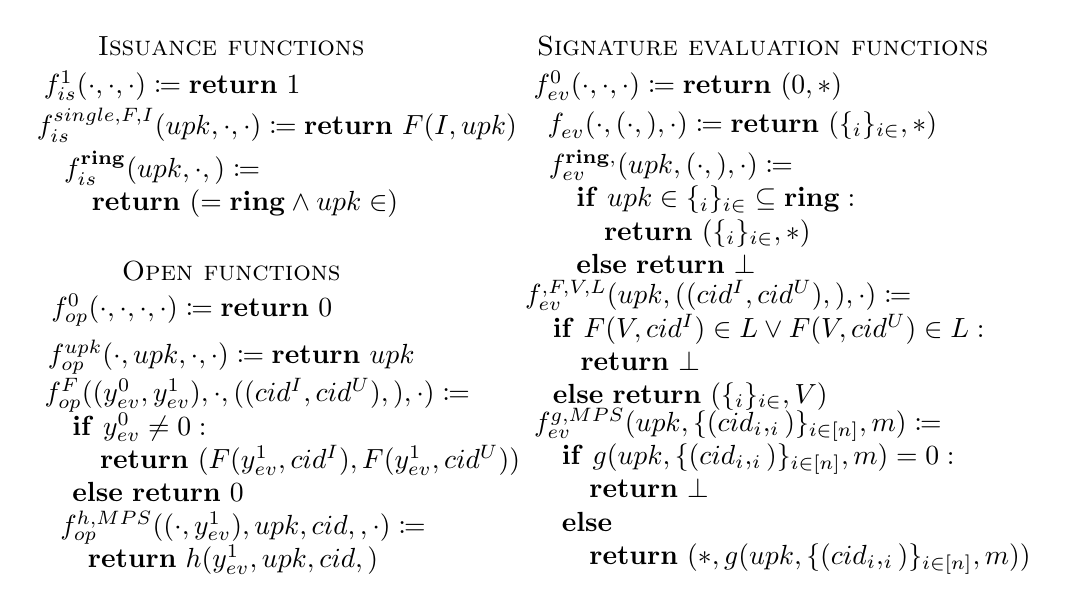
\begin{tikzpicture}

  \pgfdeclarelayer{bg}    % declare background layer
  \pgfsetlayers{bg,main}  % set the order of the layers (main is the standard layer)

  \node (issue) at (0.00,5.00) { \sc Issuance functions };
  \node (sign) at (6.75,5.00) { \sc Signature evaluation functions };  
  \node (open) at (0.00,2.15) { \sc Open functions };

  % Issue functions
  \node (fissue1) at (-0.75,4.50) {
    $\fissue^1(\cdot,\cdot,\cdot) \coloneqq \pcreturn 1$
  };
  \node (fissue2) at (0.58,4.00) {
    $\fissue^{single,F,I}(\upk,\cdot,\cdot) \coloneqq \pcreturn F(I,\upk)$
  };
  \node[align=left] (fissue3) at (0.00,3.25) {
    $\fissue^{\sring}(\upk,\cdot,\attrs) \coloneqq$ \\
    \hspace*{1em}$\pcreturn (\attrs = \sring \land \upk \in \attrs)$
  };

  % Signature evaluation functions
  \node (fsign1) at (5.80,4.50) {
    $\feval^0(\cdot,\cdot,\cdot) \coloneqq \pcreturn (0,\ast)$
  };
  \node[align=left] (fsign2) at (6.55,4.00) {
    $\feval^{\dattrs}(\cdot,(\cdot,\attrs),\cdot) \coloneqq
    \pcreturn (\lbrace \attrs_i \rbrace_{i\in \dattrs},\ast)$
  };
  \node[align=left] (fsign3) at (5.98,2.90) {
    $\feval^{\sring,\dattrs}(\upk,(\cdot,\attrs),\cdot) \coloneqq$ \\
    \hspace*{1em}$\pcif \upk \in \lbrace \attrs_i \rbrace_{i\in\dattrs}
    \subseteq \sring:$ \\
    \hspace*{2em}$\pcreturn (\lbrace \attrs_i \rbrace_{i\in\dattrs},\ast)$ \\
    \hspace*{1em}$\pcelse \pcreturn \bot$
  };
  \node[align=left] (fsign4) at (6.65,1.20) {
    $\feval^{\dattrs,F,V,L}(\upk,((\cidi,\cidu),\attrs),\cdot) \coloneqq$ \\
    \hspace*{1em}$\pcif F(V,\cidi) \in L \lor F(V,\cidu) \in L:$ \\
    \hspace*{2em}$\pcreturn \bot$ \\
    \hspace*{1em}$\pcelse \pcreturn (\lbrace \attrs_i \rbrace_{i\in \dattrs},V)$
  };
  \node[align=left] (fsign5) at (7.00,-0.65) {
    $\feval^{g,MPS}(\upk,\lbrace (\cid_i,\attrs_i) \rbrace_{i\in[n]},\msg) \coloneqq$ \\
    \hspace*{1em}$\pcif g(\upk,\lbrace (\cid_i,\attrs_i) \rbrace_{i\in[n]},
    \msg) = 0:$ \\
    \hspace*{2em}$\pcreturn \bot$ \\
    \hspace*{1em}$\pcelse$ \\
    \hspace*{2em}$\pcreturn (\ast,g(\upk,\lbrace(\cid_i,\attrs_i)
    \rbrace_{i\in[n]},\msg))$
  };

  % Open functions
  \node (fopen1) at (-0.50,1.65) {
    $\finsp^0(\cdot,\cdot,\cdot,\cdot) \coloneqq \pcreturn 0$
  };
  \node (fopen2) at (0.00,1.05) {
    $\finsp^{\upk}(\cdot,\upk,\cdot,\cdot) \coloneqq \pcreturn \upk$
  };
  \node[align=left] (fopen3) at (0.65,0.00) {
    $\finsp^{F}((\yeval^0,\yeval^1),\cdot,((\cidi,\cidu),\attrs),\cdot)
    \coloneqq$ \\
    \hspace*{1em}$\pcif \yeval^0 \neq 0:$\\
    \hspace*{2em}$\pcreturn (F(\yeval^1,\cidi),F(\yeval^1,\cidu))$ \\
    \hspace*{1em}$\pcelse \pcreturn 0$
  };
  \node[align=left] (fopen4) at (0.15,-1.30){
    $\finsp^{h,MPS}((\cdot,\yeval^1),\upk,\cid,\attrs,\cdot) \coloneqq$ \\
    \hspace*{1em}$\pcreturn h(\yeval^1,\upk,\cid,\attrs)$
  };
  
  % \draw[draw=black,thick] (5.65,2.29) rectangle ++(1.43,0.44);
  % \draw[draw=black,dashed,thick] (1.80,1.09) rectangle ++(1.75,0.44);
  % \draw[draw=black,dotted,thick] (3.85,1.09) rectangle ++(2.30,0.44);
    
\end{tikzpicture}

%%% Local Variables:
%%% mode: latex
%%% TeX-master: t
%%% End:

  }
  \caption{Functions for the \CUASGen restrictions described next.
    For readability, we use ``$\cdot$'' to denote input arguments that are
    ignored; and ``$\ast$'' to denote output values that can be set to anything
    (but should be ignored). $\bot$ means that the function fails.}
  \label{fig:func-restrictions}
\end{figure}

\subsection{Group Signatures}
\label{ssec:related-models-gs}

We adopt the model in \cite{bsz05}. In this abstraction, the opener returns an
index uniquely identifying the group member who created a signature, along with
a correctness proof. To ease exposition, we assume without loss of generality
that this index is just the public key that group members generate randomly
when joining the group\footnote{The user public key is
  assumed to be
  accessible from a public table in \cite{bsz05}, so it is easy to translate the
  public key into an index, if needed.}. A group signature scheme in
\cite{bsz05} is composed of $KeyGen$, \UKeyGen, \Sign, \Verify, \Open and
\Judge algorithms, and an $\langle\Obtain,\Issue\rangle$ interactive
protocol. Their intuition is similar to that of \UAS, so we refer to
\cite{bsz05} for detailed descriptions. For ease of reference, we replicate the
security games in \figref{fig:model-gs}.

\begin{figure}[ht!]
  \centering
  \scalebox{0.85}{      
    \begin{minipage}[t]{0.45\textwidth}        
      \procedure[linenumbering]{$\Exp^{anon-b}_{\adv,gs}(1^\secpar)$}{%
        (\gpk,\isk,\osk) \gets KeyGen(1^\secpar) \\
        d \gets \adv^{\mathcal{O}_{anon}}(\gpk,\isk) \\
        \pcreturn d 
      }
      
      \vspace*{3em}
      
      \procedure[linenumbering]{$\Exp^{frame}_{\adv,gs}(1^\secpar)$}{%
        (\gpk,\isk,\osk) \gets KeyGen(1^\secpar) \\
        (\msg,\sig,\upk,\tau) \gets \adv^{\mathcal{O}_{frame}}
        (\gpk,\osk,\isk) \\
        \pcif \Verify(\gpk,\msg,\sig) = 0: \pcreturn 0 \\
        \pcreturn \upk \in \HU \land \PRVUK[\upk] \neq \bot \land
        \Judge(\gpk,\upk,\msg,\sig,\tau) = 1~\land \\
        \pcind \adv~\textrm{did not query}~USK(\upk)~\textrm{or}~
        GSig(\PRVUK[\upk],\msg)
      }       
    \end{minipage}
  }
  \scalebox{0.85}{      
    \begin{minipage}[t]{.55\textwidth}
      \procedure[linenumbering]{$\Exp^{trace}_{\adv,gs}(1^\secpar)$}{%
        (\gpk,\isk,\osk) \gets KeyGen(1^\secpar) \\
        (\msg,\sig) \gets \adv^{\mathcal{O}_{trace}}(\gpk,\osk) \\
        \pcif \Verify(\gpk,\msg,\sig) = 0: \pcreturn 0 \\
        (\upk, \tau) \gets \Open(\gpk,\osk,\trans,\msg,\sig) \\
        \pcreturn \upk \notin \HU \cup \CU \lor \Judge(\gpk,\upk,\msg,\sig,\tau)
        = 0
      }       
    \end{minipage}      
  }
  \caption{Security games for group signatures \cite{bsz05}, only with minor    
    ``harmless'' edits to ease comparison with \CUASGS. Concretely, since we
    output {\upk}s instead of indexes, $i=0$ in the traceability game now reads
    $\upk \notin \HU \cup \CU$. For the oracles' definitions, check the
    referenced paper.
    $\mathcal{O}_{anon} \gets \lbrace \oracle{Ch},\oracle{Open},\oracle{SndToU},
    \oracle{WReg},\oracle{USK},\oracle{CrptU} \rbrace$,
    $\mathcal{O}_{trace} \gets \lbrace \oracle{SndToI},\oracle{AddU},
    \oracle{RReg},\oracle{GSig},\oracle{USK},\oracle{CrptU} \rbrace$,
    and $\mathcal{O}_{frame} \gets \lbrace \oracle{SndToU},\oracle{WReg},
    \oracle{GSig},\oracle{USK},\oracle{CrptU} \rbrace$.
  }
  \label{fig:model-gs}  
\end{figure}

\subsubsection{\CUASGS construction.} %
We show that a $(\fissue^{single,H,I},\feval^0,\finsp^{\upk})$-\CUASGen
restriction is a secure group signature scheme according to \cite{bsz05}.
As stated, $\fissue^{single,H,I}$ is an \UAS-acceptable function if $H$ is a
PRF, as its output is a random-looking string that depends on the user public
key \upk, and a string $I$ uniquely identifying the issuer. Thus, it is the same
per $(I,\upk)$ pair, and can be used by issuer $I$ to prevent issuing more than
one credential per user. Basically, the issuer keeps a list of received
$\yissue = H(I,\upk)$ values, and rejects issuing a credential for already
existing ones. From this, the GS algorithms are as follows:

\begin{description}
\item[$(\gpk,\isk,\osk) \gets KeyGen(1^\secpar)$.] Runs \Setup from \CUASGen,
  and two instances of \KeyGen. One followed by \ISet with $\fissue^{single,H,
    I}$ for the same user, who will be the issuer; and another for a different
  user, who will be the opener, followed with \OKeyGen with $\finsp^{\upk}$.
  Assigns the public keys to \gpk.
\item[$(\upk,\usk) \gets \UKeyGen(1^\secpar)$.] Runs \KeyGen from \CUASGen.
\item[$\langle \cred,\utrans \rangle \gets
  \langle\Obtain(\usk,\ipk),\Issue(\isk,\upk)\rangle$.] Runs $\langle\Obtain,
  \Issue\rangle$ as in \CUASGen, with $\attrs \gets \emptyset$. Upon receiving
  the \yissue value, the issuer checks if it already exists in a list $L$
  (initially set to $\emptyset$); if it exists, aborts issuance. Otherwise, it
  completes the protocol and adds $\yissue$ to $L$. It is responsibility of the
  issuer to maintain $L$.
\item[$\sig \gets \Sign(\gpk,\cred,\msg)$.] Parses \gpk as $(\ipk,\opk)$, and
  runs $(\sig,0) \gets \Sign(\usk,\opk,\cred,\msg,\feval^0)$ from \CUASGen,
  where $\yeval = 0$ is the constant output of $\feval^0$.
\item[$1/0 \gets \Verify(\gpk,\sig,\msg)$.] Parses \gpk as $(\ipk,\opk)$, and
  returns whatever $\Verify(\opk,\ipk,\sig,0,\msg,\feval^0)$ from \CUASGen
  outputs.
\item[$(\upk,\pi) \gets \Open(\gpk,\osk,\trans,\sig,\msg)$.] Parses \gpk as
  $(\ipk,\opk)$, and returns whatever \CUASGen outputs in $\Open(\osk,\ipk,\sig,
  0,\msg,\feval^0)$, which internally runs $\finsp^{\upk}$.
\item[$1/0 \gets \Judge(\gpk,\pi,\upk,\sig,\msg)$.] Parses \gpk as $(\ipk,
  \opk)$, and returns whatever \CUASGen outputs in $\Judge(\opk,\upk,\pi,\sig,
  0,\msg)$.
\end{description}

% \paragraph{Security of \CUASGS.} %
% Our \CUASGS construction is an anonymous, traceable, and non-frameable group
% signature scheme, according to the model in \cite{bsz05}. For space constraints,
% proofs are deferred to \appref{app:related-proofs}.

% \begin{theorem}[Anonymity of \CUASGS]
%   If the base \CUASGen construction has signature anonymity according to
%   \defref{def:sign-anonymity-uas}, then \CUASGS is an anonymous group signature
%   scheme.
% \end{theorem}

% \begin{theorem}[Traceability of \CUASGS]
%   If the base \CUASGen construction is unforgeable according to
%   \defref{def:forge-uas}, then \CUASGS is a traceable group signature scheme.
% \end{theorem}

% \begin{theorem}[Non-frameability of \CUASGS]
%   If the base \CUASGen construction is non-frameable according to
%   \defref{def:frame-uas}, then \CUASGS is a non-frameable group signature
%   scheme.
% \end{theorem}

\subsection{Ring Signatures}
\label{ssec:related-models-rs}

We adopt the model in \cite{bkm06}, where security of ring signatures is
defined according to the games in \figref{fig:model-rs}. A ring signature
scheme consists of three algorithms $(KeyGen,Sign,Verify)$. Roughly,
$((\pk_1,\sk_1),\dots,(\pk_n,\sk_n)) \gets KeyGen(1^\secpar)$ produces $n$
signing key pairs, $\sig \gets Sign(\sk_i,R,\msg)$ creates a signature for
anonymity set $R \subseteq \lbrace \pk_1, \dots, \pk_t \rbrace$, using secret
key $\sk_i$, associated to some $\pk_i \in R$; and $1/0 \gets Verify(R,\sig,
\msg)$ checks if \sig is a valid signature over \msg for ring $R$. We refer
to \cite{bkm06} for details on the syntax and definitions.

\begin{figure}[ht!]
  \centering
  \scalebox{0.85}{      
    \begin{minipage}[t]{0.55\textwidth}        
      \procedure[linenumbering]{$\Exp^{anon-b}_{\adv,rs}(1^\secpar)$}{%
        ((\pk_1,\sk_1),\dots,(\pk_n,\sk_n)) \gets KeyGen(1^\secpar) \\
        (i_0,i_1,R,\msg,\st) \gets \adv^{\oracle{Sign}}(\pk_1,\dots,\pk_n) \\
        \pcif R \not\subseteq \lbrace \pk_i \rbrace_{i\in[n]} \lor
        \lbrace \pk_{i_0},\pk_{i_1} \rbrace \not\subseteq R~\lor \\ %\\
        \pcind i_0 = i_1: \pcreturn \bot \\
        \sig \gets Sign(\sk_{i_b},R,\msg) \\
        b^* \gets \adv(\sig,\st) \\
        \pcreturn b^*
      }        
    \end{minipage}
  }
  \scalebox{0.85}{      
    \begin{minipage}[t]{.5\textwidth}
      \procedure[linenumbering]{$\Exp^{forge}_{\adv,rs}(1^\secpar)$}{%
        ((\pk_1,\sk_1),\dots,(\pk_n,\sk_n)) \gets KeyGen(1^\secpar) \\
        (R,\sig,\msg) \gets \adv^{\oracle{Sign},\oracle{Corr}}
        (\pk_1,\dots,\pk_n) \\
        \pcif Verify(R,\sig,\msg) = 0: \pcreturn 0 \\
        \pcreturn (R \subseteq \lbrace \pk_i \rbrace_{i\in[n]} \setminus
        CU~\land \\
        \pcind \adv~\textrm{never queried}~\oracle{Sign}(\cdot,R,\msg))
      }       
    \end{minipage}      
  }
  \caption{Security games for ring signatures \cite{bkm06}. The $\oracle{Sign}$
    oracle accepts $(i,R,\msg)$ tuples, with $pk_i \in R$, adds the tuple to a
    list of queries, and returns $\sig \gets Sign(\sk_i,R,\msg)$.
    $\oracle{Corr}$ accepts an index $i$, and leaks $\sk_i$. Corrupted users are
    added to $CU$.}
  \label{fig:model-rs}  
\end{figure}


\subsubsection{\CUASRing Construction.} %
We use a $(\fissue^{\sring},\feval^{\sring,\dattrs},\finsp^0)$-restriction
of \CUASGenHideIss to build a ring signature scheme in the model given in
\figref{fig:model-rs}. Briefly, users self-issue credentials where the
attributes are (encodings of) the public keys of the users in the system --
including their own public key. Then, a ring signature is just a
\CUASGenHideIss signature that reveals a subset of the attributes -- i.e., a
subset of the keys of the users in the system. The construction
is as follows:

% \begin{align}
%   & \NIZKRel_{\Sign}^{prv} \coloneqq \lbrace (\usk,\cred,\yeval^1,\yinsp,r,r',
%     \ipk),(\msg,\feval,\yeval^0,\ceval,\cinsp,\Eek,\widetilde{\Eek},\sring): \nonumber \\
%   & \hspace*{6.405em}\ceval = \EEnc(\widetilde{\Eek},\yeval^1;r) \land
%     \cinsp = \EEnc(\Eek,\yinsp;r') \land \nonumber \\
%   & \hspace*{6.40em}(\yeval^0,\yeval^1) = \feval(\usk,\cred,\msg) \land
%     \yinsp = \finsp((\yeval^0,\yeval^1),\usk,\cred,\msg) \nonumber \\
%   & \hspace*{6.40em}\exists \ipk \in \sring~\suchthat~\SBCMVerify(\ipk,\cred,\usk,
%     \sring) = 1) \rbrace \label{eq:sign-prv}
% \end{align}

% From it, we show that the $(\fissue^{\sring},\feval^{\attrs},\finsp^0)$-
% $\CUASGen^{\Sign-prv}$ restriction, is a secure ring signature scheme. We
% restrict to one credential per signature.

\begin{description}
%\item[$\parm \gets \Setup(\secpar,\AttrSpace)$.] As in \CUASGenHideIss.
\item[$((\pk_1,\sk_1),...,(\pk_n,\sk_n)) \gets KeyGen(\secpar)$.] Runs
  $\parm \gets \Setup(\secpar)$ from \CUASGenHideIss. For each of
  the $i \in [n]$ users to generate, run $(\upk_i,\usk_i) \gets \KeyGen(\parm)$,
  and $\ipk_i \gets \ISet((\upk_i,\usk_i),\fissue^{\sring})$, where $\sring =
  \lbrace \upk_i \rbrace_{i\in[n]}$. Run also $(\opk,\osk) \gets \OKeyGen(\parm,
  \finsp^0)$. Set $\pk_i \gets (\ipk_i,\opk)$ and $\sk_i \gets \usk_i$, for
  $i\in[n]$.
\item[$\Sig \gets \Sign(\sk_i,R,\msg).$]
  The signing user, with $\sk_i=\usk$ and $\pk_i=(\ipk_i,\opk)$ for some $i \in
  [n]$ where $\pk_i \in R$, first acts both as user and issuer to self-issue a
  credential \Cred over an attribute set \attrs such that $\attrs = \sring$. The
  user picks some \dattrs such that $\dattrs \subseteq [|\attrs|]$, and computes
  the ring signature by running $\Sig = (\sig,\yeval) \gets
  \Sign(\usk,\opk,\Cred,\msg,\feval^{\sring,\dattrs})$ from
  \CUASGenHideIss. Note that \dattrs defines the public keys within
  $\attrs = \sring$ to be revealed through \yeval.
\item[$1/0 \gets Verify(R,\Sig,\msg)$.] Parses \Sig as $(\sig,\yeval)$ and
  runs $\Verify(\opk,\yeval,\Sig,\msg,\feval^{\sring,\dattrs})$ as in
  \CUASGenHideIss. Note that, in valid signatures, $\yeval = \lbrace
  \ipk_i\rbrace_{i\in\dattrs}$.
\end{description}

%Note that by using, e.g., $\finsp^{\upk}$, we essentially get a ring signature
%scheme with linkability via an opener.

% \paragraph{Security of \CUASRing.} %
% Our \CUASRing construction is an anonymous and unforgeable ring signature
% scheme, according to the model in \cite{bkm06}. For space constraints,
% proofs are deferred to \appref{app:related-proofs}.

% \begin{theorem}[Anonymity of \CUASRing]
%   If the base \CUASGenHideIss construction has signature anonymity
%   according to \defref{def:sign-anonymity-uas}, then \CUASRing is an anonymous
%   ring signature scheme.
% \end{theorem}

% \begin{theorem}[Unforgeability of \CUASRing]
%   If the base \CUASGenHideIss construction is non-frameable according to
%   \defref{def:frame-uas}, then \CUASRing is an unforgeable ring signature
%   scheme.
% \end{theorem}

\subsection{Anonymous Credentials}
\label{ssec:related-models-ac}

We adopt the model in \cite{fhs19} for anonymous credentials with selective
disclosure, which restricts to one credential per presentation. Therein, an
anonymous credential scheme is defined via $OrgKeyGen$ (which we rename to
$IssKeyGen$), and $UserKeyGen$ algorithms, and $\langle Obtain,Issue\rangle$
and $\langle Show,Verify \rangle$ interactive protocols. We
refer to \cite{fhs19} for the full details. For readability, we give
the security definitions in \figref{fig:model-ac}.% , with inocuous
% adaptations to make them more suitable for comparison with our definitions --
% namely, we explicitly add a common setup process which is part of $IssKeyGen$
% in \cite{fhs19}.

\begin{figure}[ht!]
  \centering
  \scalebox{0.85}{      
    \begin{minipage}[t]{0.5\textwidth}        
      \procedure[linenumbering]{$\Exp^{anon-b}_{\adv,ac}(1^\secpar)$}{%
 %       \parm \gets \Setup(1^\secpar) \\
        (\ipk,\isk) \gets IssKeyGen(1^\secpar) \\        
        b^* \gets \adv^{\oracle{HU},\oracle{CU},\oracle{Obtain},
          \oracle{Show},\oracle{LoR}}(\isk) \\
        \pcreturn b^*
      }        
    \end{minipage}
  }
  \scalebox{0.85}{      
    \begin{minipage}[t]{.5\textwidth}
      \procedure[linenumbering]{$\Exp^{forge}_{\adv,ac}(1^\secpar)$}{%
%        \parm \gets \Setup(1^\secpar) \\
        (\ipk,\isk) \gets IssKeyGen(1^\secpar) \\        
        (D,\st) \gets \adv^{\oracle{HU},\oracle{CU},\oracle{ObtIss},
          \oracle{Issue},\oracle{Show}}(\ipk) \\
        \langle \cdot,(b,\utrans) \rangle
        \gets \langle \adv(\st),\Verify(\ipk,D) \rangle \\
        \pcreturn (b = 1 \land \nexists j~\suchthat \\
        \pcind (\OWNR[j] \in \CU
        \land D \subseteq \ATTR[j])) % \forall j, \OWNR[j] \in \CU
        % \implies D \not\subseteq \ATTR[j]: \\
        %\pcind \pcreturn 1 \\
        %\pcreturn 0
      }       
    \end{minipage}      
  }
  \caption{Games for anonymous credentials with selective disclosure
    \cite{fhs19}. \OWNR, \ATTR, and the oracles, are essentially as in
    \UAS. \adv~wins $\Exp^{forge}_{\adv,ac}$ if it authenticates successfully
    while revealing attributes not contained in adversarially controlled
    credentials.}
  \label{fig:model-ac}  
\end{figure}

\subsubsection{\CUASAC Construction.} %
We build a secure anonymous credential scheme directly from a
$(\fissue^1,\feval^{\dattrs},\finsp^0)$-\CUASGenInt restriction.

\begin{description}
% \item[$\parm \gets \Setup(1^\secpar)$.] Runs $\parm' \gets \Setup(1^\secpar,
%   \AttrSpace)$ and $(\opk,\osk) \gets \OKeyGen(\parm',\finsp^0)$ from our
%   \CUASGen construction. Returns $\parm \gets (\parm',\opk)$.
\item[$(\ipk,\isk) \gets IssKeyGen(\parm)$.] From \CUASGenInt, run $\parm'
  \gets \Setup(1^\secpar)$ and $(\opk,\osk) \gets \OKeyGen(\parm',
  \finsp^0)$, and set $\parm \gets (\parm',\opk)$. Run $(\upk,\usk) \gets
  \KeyGen(\parm')$ and $\ipk \gets \ISet(\upk,\usk,\fissue^1)$. Set $\isk \gets
  \usk$.
\item[$(\upk,\usk) \gets UserKeyGen(\ipk)$.] Runs \KeyGen from \CUASGenInt.
\item[$\langle \cred/\bot,\top/\bot \rangle \gets
  \langle \Obtain(\usk,\ipk,\attrs),\Issue(\isk,\upk,\attrs) \rangle$.]
  Runs $\langle \Obtain,\Issue \rangle$ from \CUASGenInt.
\item[$\langle 1/0,((\yeval,\utrans)/(0,\utrans)\rangle
  \gets \langle Show(\ipk,\attrs,\dattrs,
  \cred),\Verify(\ipk,\dattrs) \rangle$.]
  Runs the interactive $\langle \Sign, \Verify\rangle$ of  \CUASGenInt,
  using $\feval^{\dattrs}$ as evaluation function, and $\finsp^0$ as
  open function, with \opk from \parm as opener public key. The \yeval value
  output by \Verify, when it accepts, is the $\yeval^0$ value output by
  \Sign in \CUASGenInt.
\end{description}

% \paragraph{Security of \CUASAC.} %
% Our \CUASAC construction is an anonymous and unforgeable anonymous credential
% scheme, according to the model in \cite{fhs19}. For space constraints,
% proofs are deferred to \appref{app:related-proofs}.

% \begin{theorem}[Anonymity of \CUASAC]
%   \label{thm:anon-cuasac}
%   If the base \CUASGenInt construction has signature anonymity according to
%   \defref{def:sign-anonymity-uas}, then \CUASAC is an anonymous AC scheme
%   according to \cite{fhs19}.
% \end{theorem}

% \begin{theorem}[Unforgeability of \CUASAC]
%   \label{thm:forge-cuasac}
%   If the base \CUASGenInt construction is unforgeabile according to
%   \defref{def:forge-uas}, then \CUASAC is an unforgeable AC scheme.
% \end{theorem}

%%% Local Variables:
%%% mode: latex
%%% TeX-master: "uas-paper"
%%% End:

\section{Conclusion}
\label{sec:conclusion}

We present a general model for privacy-preserving signatures and authentication,
and provide a generic construction, secure in our model, that allows
different privacy-vs-utility tradeoffs to be reached.
%
Then, we prove that well-known schemes are special cases of our generic
construction. The implied schemes include group signatures, anonymous
credentials (with and without revocation), ring signatures, or the recently
proposed multimodal private signatures.

Flexibility in our model is achieved via functional placeholders that
modulate the behaviour at credential issuance time, the utility
information revealed along with the produced signatures, and the utility
information extractable from already produced signatures. These functions are
computed by the users, who prove correct computation. We include features of
anonymous credential schemes, like attributes and multiple
issuers, which we extend with openers (like in group signatures), enabling
multiple openers to coexist. This further increases flexibility, by removing
the tight issuer-opener coupling in previous works.

For future work, an obvious line is to come up with (and implement) concrete
instantiations of our generic construction in order to evaluate efficiency in
real-world use cases. Alternative generic constructions are also of interest --
for instance, based on structure-preserving signatures.
%
Finally, in this work we focus only on utility over \emph{one} signature. But
extending our model and constructions to span utility over \emph{multiple}
signatures promises to be interesting, both regarding its modelling, the
potential use cases, and the generalization capabilities.


%%% Local Variables:
%%% mode: latex
%%% TeX-master: "uas-paper"
%%% End:


\bibliographystyle{splncs04}
\bibliography{uas-paper}

\appendix

\section{Cryptographic Building Blocks}
\label{app:crypto-building-blocks}

\iffalse
\subsection{Digital Signatures}
\label{sapp:digital-signatures}

We rely on digital signatures as a core building block. A digital signature
provides the functionality defined by the following syntax:

\begin{description}
\item[$\Sparm \gets \SSetup(\Ssecpar)$.] It produces public parameters for the
  other algorithms, given an input security parameter \Ssecpar.
\item[$(\Svk,\Ssk) \gets \SKeyGen(\Sparm)$.] Generates a verification-signing
  key pair.
\item[$\Ssig \gets \SSign(\Ssk,\msg)$.] Signs message \msg with signing key
  \Ssk, producing signature \Ssig,  
\item[$1/0 \gets \SVerify(\Svk,\Ssig,\msg)$.] Checks whether \Ssig is a valid
  signature over \msg, under verification key \Svk.
\end{description}

A digital signature scheme is correct if honestly generated signatures, using
honestly generated key pairs, are always accepted by \SVerify. 
%
A digital signature scheme \S has existential unforgeability if, for all p.p.t.
adversaries $\adv$, $\Pr[\ExpEUF(\Ssecpar) = 1]$ is a negligible function of the
security parameter.

\begin{figure}[ht!]
  \scalebox{0.9}{  
    \begin{minipage}[t]{\textwidth}
      \centering
      \procedure{$\ExpEUF(\Ssecpar)$}{%
        \Sparm \gets \SSetup(\Ssecpar) \\
        (\Svk,\Ssk) \gets \SKeyGen(\Sparm) \\
        (\Ssig,\msg) \gets \adv^{\SSign(\Ssk,\cdot)}(\Svk) \\
        \pcif \SVerify(\Svk,\Ssig,\msg) = 0: \pcreturn 0 \\
        \pcif \msg~\textrm{was not queried to \SSign}: \pcreturn 1 \\
        \pcreturn 0
      }
    \end{minipage}
  }
  \label{fig:euf-game}
  \caption{Existential Unforgeability Game.}
\end{figure}
\fi

\subsection{Public-Key Encryption}
\label{sapp:pk-encryption}

A public-key encryption scheme is defined by the following algorithms:

\begin{description}
\item[$\Eparm \gets \ESetup(\Esecpar)$.] Produces public parameters \Eparm given
  a security parameter \Esecpar.
\item[$(\Eek,\Edk) \gets \EKeyGen(\Eparm)$.] Given public parameters \Eparm,
  produces an encryption-decryption key pair $(\Eek,\Edk)$.
\item[$\Ec \gets \EEnc(\Eek,\msg)$.] Encrypts message \msg with encryption key
  \Eek, producing ciphertext \Ec.
\item[$\msg \gets \EDec(\Edk,\Ec)$.] Decrypts ciphertext \Ec with decryption key
  \Edk.
\end{description}

A public-key encryption scheme is correct if, given a honestly generated key
pair $(\Eek,\Edk)$, produced with honestly generated parameters \Eparm,
$\Pr[\EDec(\Edk,\EEnc(\Eek,\msg))=\msg] = 1$ with overwhelming probability.

A public-key encryption scheme has IND-CCA2 security if
$\Pr[\ExpINDCCAiio(\Esecpar) = 1] - \Pr[\ExpINDCCAiiz(\Esecpar) = 1]|$ is
a negligible function of \Esecpar, for any p.p.t. adversary \adv, where
\ExpINDCCAiib is as defined in \figref{fig:indcca2-game}.

\begin{figure}[ht!]
  \scalebox{0.9}{  
    \begin{minipage}[t]{\textwidth}
      \centering      
      \procedure{$\ExpINDCCAiib(\Esecpar)$}{%
        \Eparm \gets \ESetup(\Esecpar) \\
        (\Eek,\Edk) \gets \EKeyGen(\Eparm) \\
        b^* \gets \adv^{\ELR(b,\cdot,\cdot),\EDEC(\Edk,\cdot)}(\Eek),
        ~\textrm{where:} \\
        \pcind \ELR(b,\msg_0,\msg_1)~\textrm{returns}~\EEnc(\Eek,\msg_b),
        ~\textrm{and} \\
        \pcind \EDEC(\Edk,\Ec)~\textrm{returns}~\EDec(\Edk,\Ec) \\
        \pcif \EDEC~\textrm{has been called with an output of \ELR, abort} \\
        \pcreturn b^*
      }
    \end{minipage}
  }
  \label{fig:indcca2-game}
  \caption{IND-CCA2 Game.}
\end{figure}

\subsection{Commitments}
\label{sapp:commitments}

Although we don't expose commitments directly in our \UAS scheme or
constructions, they are an essential part of \SBCM schemes. Thus, we overview
them briefly next. In a nutshell, a commitment scheme is defined by the
following algorithms:

\begin{description}
\item[$\Cparm \gets \CSetup(\Csecpar)$.] Given a security parameter \Csecpar,
  returns the public parameters \Cparm to commit messages.
\item[$\Ccom \gets \CCommit(\Cparm,\msg;r)$.] Given the public parameters and
  a message \msg, outputs a commitment \Ccom to \msg, for which randomness $r$
  from some predefined randomness space $\mathcal{R}$ is used.
\end{description}

Opening a commitment \Ccom means revealing the message \msg and randomness $r$
that were used to produce \Ccom. Commitment schemes are required to be binding
and (usually) hiding:

\begin{description}
\item[Binding.] Intuitively, the binding property of commitment schemes means
  that no adversary can change the message that has been committed to. More
  formally, $\Pr[\ExpComBind(\Csecpar) = 1]$ must be a negligible function of
  the security parameter.
\item[Hiding.] The hiding property captures that no adversary should be able to
  learn the message that was committed, when given only the commitment. This is
  formally defined through \ExpComHideb, where $|\Pr[\ExpComHideb(\Csecpar)=1|
  b=1] - \Pr[\ExpComHideb(\Csecpar)=1|b=0]|$ must be a negligible function of
  the security parameter.
\end{description}

\begin{figure}[ht!]
  \scalebox{0.9}{
    \begin{minipage}[t]{0.5\textwidth}
      \procedure{$\ExpComBind(\Csecpar)$}{%
        \Cparm \gets \CSetup(\Csecpar) \\
        (\msg_0,r_0,\msg_1,r_1) \gets \adv(\Cparm) \\
        \Ccom_0 \gets \CCommit(\Cparm,\msg_0,r_0) \\
        \Ccom_1 \gets \CCommit(\Cparm,\msg_1,r_1) \\
        \pcif \msg_0 \neq \msg_1 \land \Ccom_0 = \Ccom_1: \pcreturn 1 \\
        \pcreturn 0
      }
    \end{minipage}
    \begin{minipage}[t]{0.5\textwidth}
      \procedure{$\ExpComHideb(\secpar)$}{%
        \Cparm \gets \CSetup(\secpar) \\
        b' \gets \adv^{COM(\Cparm,\cdot,\cdot)},~\textrm{where}: \\
        \pcind COM(\Cparm,\msg_0,\msg_1): \\
        \pcind \pcind r \getr \mathcal{R};~\pcreturn \CCommit(\Cparm,\msg_b,r) \\
        % (\msg_0,\msg_1,st) \gets \adv(\Cparm) \\
        % r \getr \mathcal{R} \\
        % \Ccom \gets \CCommit(\Cparm,\msg_b,r) \\
        % b' \gets \adv(st,\Ccom) \\
        \pcreturn b'
      }
    \end{minipage}
  }
  \label{fig:com-games}
  \caption{Games for commitment schemes.}
\end{figure}

\paragraph{Commitments on Blocks of Messages.} We also use an extension
of commitment schemes that allows committing to multiple messages at once. The
properties we need are the same, and their definitions are extended in the
natural way. Namely, $\CCommit$ receives a vector/block of messages, \msgset
instead of a single message. In the games, the adversary returns sets of
messages and, in the binding game, the comparison $\msg_0 \neq \msg_1$ now
compares sets $\msgset_0$ and $\msgset_1$, which must differ in at least one
element. This extension is straight-forward, for instance, from Pedersen
commitments \cite{bcc+15}.

\subsection{Simulation-Extractable Non-Interactive Zero-Knowledge
  Proofs of Knowledge}
\label{sapp:nizk}

Let \NIZKRel be an NP relation defined by pairs of elements $(\NIZKx,\NIZKw)$,
where \NIZKx is a statement and \NIZKw a witness proving that $(\NIZKx,\NIZKw)
\in \NIZKRel$. For concrete relations, we write $\NIZKRel = \lbrace (\NIZKx),
(\NIZKw): f(x,w) \rbrace$, where $f(x,w)$ is a Boolean predicate denoting the
concrete conditions that \NIZKx and \NIZKw need to meet. The set of all \NIZKx
such that there exists a \NIZKw for which $(\NIZKx,\NIZKw) \in \NIZKRel$ is the
language, or \NIZKLang, for \NIZKRel. $\NIZKx \notin \NIZKLang$ means that
there is no $\NIZKw$ such that $(\NIZKx,\NIZKw) \in \NIZKRel$.

We use non-interactive zero-knowledge proofs of knowledge (NIZKPoK, or, for
short, NIZK) over NP relations, in the Common Reference String (CRS) model. A
NIZK system is a tuple $(\NIZKSetup,\NIZKProve,\NIZKVerify)$, defined as follows
\cite{gos06}:

\begin{description}
\item[$\NIZKcrs \gets \NIZKSetup(\NIZKsecpar)$.] Generates a CRS \NIZKcrs from
  security parameters \NIZKsecpar.
\item[$\NIZKproof \gets \NIZKProve(\NIZKcrs,\NIZKx,\NIZKw)$.] Given \NIZKcrs,
  statement \NIZKx, and witness \NIZKw, creates a proof \NIZKproof.
\item[$1/0 \gets \NIZKVerify(\NIZKcrs,\NIZKproof,\NIZKx)$.] Checks whether
  \NIZKproof is a valid proof for \NIZKx.
\end{description}

Any zero-knowledge proof of knowledge must meet completeness, soundness and
zero-knowledge,properties. We further need an extra property, called
\emph{simulation-extractability} \cite{cl06}, which amplifies the security
requirements of (simulation-) soundness.
%
To define more formally the properties we need, we have to define three extra
algorithms:

\begin{description}
\item[$(\NIZKcrs,\NIZKtrap) \gets \NIZKSimSetup(\NIZKsecpar)$.] Produces a
  \NIZKcrs as the \NIZKSetup algorithm, along with a trapdoor \NIZKtrap.
\item[$\NIZKproof \gets \NIZKSim(\NIZKcrs,\NIZKtrap,\NIZKx)$.] Given a trapdoor
  \NIZKtrap produced by \NIZKSimSetup, and a statement $\NIZKx \in \NIZKLang$,
  produces a simulated proof \NIZKproof of $\NIZKx \in \NIZKLang$.
\item[$\NIZKw \gets \NIZKExtract(\NIZKcrs,\NIZKtrap,\NIZKx,\NIZKproof)$.] Given
  a trapdoor \NIZKtrap produced by \NIZKSimSetup, and a proof \NIZKproof for
  $\NIZKx \in \NIZKLang$, returns a valid \NIZKw for \NIZKx.
\end{description}

When we want to make explicit the NP relation \NIZKRel to which the previous
algorithms refer to, we use $\NIZKSetup^\NIZKRel,\NIZKProve^\NIZKRel$, 
$\NIZKVerify^\NIZKRel$, etc., and omit the \NIZK prefix and super-index when
clear from context. Altogether, the tuple $(\Setup,\Prove,\Verify,\SimSetup,
\Sim,\Extract)$ needs to meet the following properties:

\paragraph{Completeness.} %
Ensures that, for any $(\NIZKx,\NIZKw) \in \NIZKRel$, any honest prover will be
able to create a proof \NIZKproof that is accepted by any honest verifier, with
overwhelming probability. More precisely, $\Pr\lbrack\ExpNIZKComp(\NIZKsecpar)
\rbrack = 1$ with overwhelming probability, for any p.p.t. \adv, for
\ExpNIZKComp in \figref{fig:nizk-games}.

\paragraph{Soundness.} %
Ensures that no adversary can create proofs accepted by \Verify, for
statements $\NIZKx \notin \NIZKLang$, except with negligible probability. That
is, for \ExpNIZKSound as in \figref{fig:nizk-games}, $\Pr\lbrack\ExpNIZKSound
(\NIZKsecpar)\rbrack=1$ with overwhelming probability. If this holds only
against p.p.t. adversaries, we talk of Non-Interactive \emph{arguments}, while
if soundness holds even against unbounded adversaries, we talks about
Non-Interactive proofs.

\paragraph{Zero-knowledge.} %
Intuitively, captures that no information can be learned from a statement and
proof pair, beyond their validity (or not). This is captured by requiring the
adversary to distinguish between a run in the real world ($b=0$), where the
setup is done with \Setup, and $\adv$ has access to an honest prover
\Prove; and a run in an ideal world ($b=1$), where the setup is replaced by
\SimSetup, and proofs are simulated with the help of the trapdoor produced by
\SimSetup, except when $\adv$ specifies $(\NIZKx,\NIZKw) \notin \NIZKRel$. Note
that, in the context of simulation-extractable NIZK, this property not only
requires that the simulated proofs are indistinguishable to the real ones; it
also requires that \SimSetup is indistinguishable from \Setup. All this is
formalised by requiring that $|\Pr[\ExpNIZKZKb(\NIZKsecpar) = 1 | b = 1] -
\Pr[\ExpNIZKZKb(\NIZKsecpar) = 1 | b = 0]$ be a negligible function of \secpar,
where \ExpNIZKZKb is as defined in \figref{fig:nizk-games}.

\paragraph{Simulation-Extractability.} As stated, simulation-extractability
is an extension to simulation soundness. In a nutshell,
simulation-extractability requires that, even after having received a polynomial
number of simulated proofs of knowledge, no adversary can output a valid proof
of knowledge from which no witness can be extracted. It implies simulation
soundness, which ``just'' requires that no adversary can produce a valid proof
after having seen polynomially many simulated proofs (but does not guarantee
extraction). Formally, for simulation-extractability we require that
$\Pr[\ExpNIZKSimExt(\NIZKsecpar)] = 1$ is a negligible function of \secpar,
where \ExpNIZKSimExt is defined in \figref{fig:nizk-games}.

\begin{figure}[ht!]
  \scalebox{0.9}{
    \begin{minipage}[t]{0.5\textwidth}
      \procedure{$\ExpNIZKComp(\NIZKsecpar)$}{%
        \NIZKcrs \gets \Setup(\NIZKsecpar) \\
        (\NIZKx,\NIZKw) \gets \adv(\NIZKcrs) \\
        \pcif (\NIZKx,\NIZKw) \notin \NIZKRel: \pcreturn 0 \\
        \NIZKproof \gets \Prove(\NIZKcrs,\NIZKx,\NIZKw) \\
        b \gets \Verify(\NIZKcrs,\NIZKproof,\NIZKx) \\
        \pcreturn b \\
      }
      \procedure{$\ExpNIZKSimExt(\NIZKsecpar)$}{%
        (\NIZKcrs,\NIZKtrap) \gets \SimSetup(\NIZKsecpar) \\
        (\NIZKx,\NIZKproof) \gets \adv^{\Sim'(\NIZKcrs,\NIZKtrap,\cdot,\cdot)}
        (\NIZKcrs) \\
        \pcind \textrm{Where}~\Sim'(\NIZKcrs,\NIZKtrap,\NIZKx,\NIZKw)~\textrm{returns} \\
        \pcind \pcind
        \Sim(\NIZKcrs,\NIZKtrap,\NIZKx)~\pcif (\NIZKx,\NIZKw) \in \NIZKRel \\
        \pcind \pcind \bot~\pcif (\NIZKx,\NIZKw) \notin \NIZKRel \\
        \NIZKw' \gets \Extract(\NIZKcrs,\NIZKtrap,\NIZKx,\NIZKproof) \\
        \pcif \Verify(\NIZKcrs,\NIZKproof,\NIZKx) = 1 \land
        (\NIZKx,\NIZKw') \notin \NIZKRel~\land \\
        \pcind \NIZKx~\textrm{was not queried to $\Sim$ via $\Sim'$}: \\
        \pcind \pcreturn 1 \\
        \pcreturn 0
      }    
    \end{minipage}
    \begin{minipage}[t]{0.5\textwidth}
      \procedure{$\ExpNIZKSound(\NIZKsecpar)$}{%
        \NIZKcrs \gets \Setup(\NIZKsecpar) \\
        (\NIZKproof,\NIZKx) \gets \adv(\NIZKcrs) \\
        \pcif \NIZKx \notin \NIZKLang \land
        \Verify(\NIZKcrs,\NIZKproof,\NIZKx): \\
        \pcind \pcreturn 0 \\
        \pcreturn 1 \\
      }
      
      \procedure{$\ExpNIZKZKb(\NIZKsecpar)$}{%
        \pcif b = 0: \\
        \pcind \NIZKcrs \gets \Setup(\NIZKsecpar) \\
        \pcind \pcreturn \adv^{\Prove(\NIZKcrs,\cdot,\cdot)}(\NIZKcrs) \\
        \pcif b = 1: \\
        \pcind (\NIZKcrs,\NIZKtrap) \gets \SimSetup(\secpar) \\
        \pcind \pcreturn \adv^{\Sim'(\NIZKcrs,\NIZKtrap,\cdot,\cdot)}(\NIZKcrs),~
        \textrm{where} \\
        \pcind \Sim'(\NIZKcrs,\NIZKtrap,\NIZKx,\NIZKw)~\textrm{returns} \\
        \pcind \pcind \Sim(\NIZKcrs,\NIZKtrap,\NIZKx)~\pcif (\NIZKx,\NIZKw)
        \in \NIZKRel \\
        \pcind \pcind \bot~\pcif (\NIZKx,\NIZKw) \notin \NIZKRel
      }    
    \end{minipage}
  }
  \label{fig:nizk-games}
  \caption{Games for Simulation-Extractable NIZK schemes.}
\end{figure}

As studied in \cite{cl06}, simulation-extractable NIZKPoKs formalise the concept
of ``signatures of knowledge'' (see, e.g., \cite{cs97}). Which basically means
that, given an $(\NIZKx,\NIZKw)$ pair from an NP relation, we can treat \NIZKx
as a public key, and \NIZKw as its corresponding private key, and leverage them
to build digital signature schemes -- with the advantage of being able to do so
while proving arbitrary claims, as long as they can be represented as an NP
relation. We note that, given a simulation-extractable NIZK system, it is
straightforward to build a signature of knowledge by adding the message to be
signed in the statement of the NIZK.

\iffalse
\subsection{Signatures over Blocks of Messages}
\label{sapp:sbm}

A signature scheme on blocks of messages (\SBM) allows a signer to create a
single signature over a set of messages. The resulting signature is typically
more concise than just creating multiple signatures, and typical schemes
\cite{cl02,asm06,ps16} are additionally compatible with efficient proof
protocols over the signed messages. The functionality offered by an \SBM scheme
is as follow:

\begin{description}
\item[$\SBMparm \gets \SBMSetup(\SBMsecpar)$.] It produces public parameters
  for the other algorithms, given an input security parameter \SBMsecpar.
\item[$(\SBMvk,\SBMsk) \gets \SBMKeyGen(\SBMparm)$.] Generates a
  verification-signing key pair.
\item[$\SBMsig \gets \SBMSign(\SBMsk,\smsg)$.] Produces a signature \sig, over
  a block of messages \smsg, using signing key \SBMsk.
\item[$1/0 \gets \SBMVerify(\SBMvk,\SBMsig,\widetilde{\smsg})$.] Checks
  whether \SBMsig is a valid signature over the set of messages \smsg, under
  verification key \SBMvk.
\end{description}

An \SBM scheme must satisfy correctness and unforgeability properties.

\paragraph{Correctness.} %
Informally, an \SBM scheme is correct if signatures generated between an honest
party running running \SBMSign over \smsg, for honestly generated parameters
and key pairs, results in a signature over $\smsg \cup \overline{\smsg}$ that is
accepted by \SBMVerify.

\paragraph{Unforgeability.} %
It must be unfeasible for an adversary to produce signatures over blocks of
messages that have not been signed by the signer. More formally, an \SBM scheme
is unforgeable if, for all p.p.t. adversaries $\adv$, $\Pr[\ExpSBMEUF
(\SBMsecpar) = 1]$, as defined in \figref{fig:sbm-games}, is a negligible
function of the security parameter. 

\begin{figure}[ht!]
  \scalebox{0.9}{
    \begin{minipage}[t]{\textwidth}
      \centering    
      \procedure{$\ExpSBMEUF(\SBMsecpar)$}{%
        \SBMparm \gets \SBMSetup(\SBMsecpar) \\
        (\SBMvk,\SBMsk) \gets \SBMKeyGen(\SBMparm) \\
        (\SBMsig,\smsg) \gets \adv^{\SSign(\SBMsk,\cdot)}(\SBMvk) \\
        \pcif \SBMVerify(\SBMvk,\SBMsig,\smsg) = 0: \pcreturn 0 \\
        \pcif \smsg~\textrm{was not queried to \SBMSign}: \pcreturn 1 \\
        \pcreturn 0
      }
    \end{minipage}
  }
  \label{fig:sbm-games}
  \caption{Unforgeability game for \SBM schemes.}
\end{figure}
\fi

\subsection{Signatures over Blocks of Committed Messages}
\label{sapp:sbcm}

For our generic constructions, we use interactive signing protocols between a
user and a signer, where the user has a block of messages to sign blindly, and
both receive a common block of messages to be also included in the resulting
signature. This is precisely the case of partially blind signatures, that
collapse to blind signatures when there is no common message between user
and signer; and to conventional signatures when the user does not input a
message to be blindly signed \cite{ao00}. Partially blind signatures, as
blind signatures \cite{ps96}, cannot be modelled with the conventional security
against existential forgeries. Simply because the user is actually expected to
be able to create signatures on messages unknown to the signer, which formally
translates into the impossibility to check whether a signature output by the
adversary is over a message that has been queried to the signing oracle or not.
Thus, instead of using the conventional existential unforgeability property,
(partially) blind signature schemes move to the ``one-more'' paradigm, which
demands that no adversary can produce $n+1$ distinct signatures after having
interacted with the signing oracle at most $n$ times.

To the best of our knowledge, models of existing schemes for signing blocks of
messages like \cite{cl02,asm06,ps16,cdl16b} target the case of signing blocks
of \emph{plain} messages, and are subsequently informally extended to support
signing commitments to blocks of messages via interactive protocols. However,
they do not support signing both committed and plain messages (although the
extension is trivial); and, more importantly, do not give security models of
the resulting construction, nor of course prove its security. While extending
the constructions seems straightforward, the modelling needs to be changed due
to the mentioned nuance of the conventional EUF notion not being compatible with
interactive signing protocols where the signer does not learn (some of) the
signed message(s). As we use this variant as a generic building block,
we briefly model such a scheme for Signatures over Blocks of Committed Messages
(\SBCM).

The syntax for an \SBCM scheme is as follows:

\begin{description}
\item[$\SBCMparm \gets \SBCMSetup(\SBCMsecpar)$.] It produces public parameters
  for the other algorithms, given an input security parameter \SBCMsecpar.
\item[$(\SBCMvk,\SBCMsk) \gets \SBCMKeyGen(\SBCMparm)$.] Generates a
  verification-signing key pair.
\item[$(\SBCMcom,\pi,r) \gets \SBCMBlind(\SBCMvk,\osmsg,\smsg)$.] A user
  computes commitment \SBCMcom to request a signature over messages \osmsg (in
  committed form) and \smsg (in plain form), to signer with verification key
  \SBCMvk. The output is the commitment \SBCMcom, the randomness $r$ used to
  compute it, and a proof $\pi$ proving knowledge of \osmsg and \smsg in
  \SBCMcom.
\item[$\SBCMbsig \gets \SBCMSign(\SBCMsk,\SBCMcom,\pi,\smsg)$.] The
  signer, with signing key \SBCMsk, produces a blind signature \SBCMbsig over
  the messages committed to in commitment \SBCMcom, as well as the messages in
  \smsg, with associated proof $\pi$.
\item[$\SBCMsig \gets \SBCMUnblind(\SBCMvk,\SBCMbsig,\SBCMcom,r,\osmsg,\smsg)$.]
  A user, who requested a signature over \osmsg and \smsg, where \SBCMcom is a
  commitment over \osmsg using randomness $r$, finalises the signature,
  computing \SBCMsig from the signer's partial signature \SBCMbsig.
\item[$1/0 \gets \SBCMVerify(\SBCMvk,\SBCMsig,\osmsg,\smsg)$.] Checks
  whether \SBCMsig is a valid signature over the set of messages \osmsg and
  \smsg, under verification key \SBCMvk.
\end{description}

The correctness and security properties are then defined as follows.

\paragraph{Correctness.} %
Informally, an \SBCM scheme is correct if signatures generated between an honest
party running \SBCMBlind, an honest signer running \SBCMSign fed with the output
of \SBCMBlind and matching \smsg and signing key pair, and the user finally
running \SBCMUnblind over the partial signature by the signer and leveraging
the same randomness as in \SBCMBlind, produces a signature over \osmsg and \smsg
that is accepted by \SBCMVerify. 

\paragraph{Unforgeability.} %
It must be unfeasible for an adversary to produce signatures over blocks of
messages that have not been signed (in plain, or committed shape) by the
signer. More formally, an \SBCM scheme is unforgeable if, for all p.p.t.
adversaries $\adv$, $\Pr[\ExpSBCMOMF(\SBCMsecpar) = 1]$, as defined in
\figref{fig:sbcm-games}, is a negligible function of the security parameter.
Note that this follows the ``one-more-forgery'' type of definition of blind
signatures \cite{bold02}.

\paragraph{Blindness.} %
Finally, the signer must not learn the plaintext values of the messages that are
signed in committed form. Note that this is a weaker notion than the usual
blindness property of (partially) blind signature schemes, where it is
additionally required that the adversary cannot link a signature to the signing
process that produced it. Informally, we capture this basically as the blinding
notion of a commitment scheme -- and formally define it in \ExpSBCMBlindb in
\figref{fig:sbcm-games}.
%
Note that, in the definition, we explicitly do not give back to the adversary
\adv~any full signature (i.e., after running \SBCMUnblind) obtained from values
returned by \adv, as this will allow the adversary to trivially check what
messages (among the ones he chose) was signed. While this may seem a too weak
notion, it is good enough for our needs, as in our \UAS construction we never
share actual signatures, but zero-knowledge proofs of knowledge of such
signatures.

An \SBCM scheme is blind if, for all p.p.t.
adversaries $\adv$, $|\Pr[\ExpSBCMBlindo(\SBCMsecpar) = 1] -
\Pr[\ExpSBCMBlindz(\SBCMsecpar) = 1]|$ is a negligible function of the security
parameter.

\begin{figure}[ht!]
  \scalebox{0.85}{
    \begin{minipage}[t]{0.62\textwidth}
      \centering      
      \procedure[linenumbering]{$\ExpSBCMOMF(\secpar)$}{%
        \parm \gets \Setup(\secpar) \\
        (\vk,\sk) \gets \KeyGen(\parm) \\
        \lbrace(\sig_i,\overline{\smsg}_i, \smsg_i)\rbrace_{i\in[n]} \gets
        \adv^{\Sign(\sk,\cdot,\cdot,\cdot)}(\vk) \\
        \pcif \exists i \in [n]~\st~\Verify(\vk,\sig_i,\osmsg_i,\smsg_i) = 0: \\
        \pcind \pcreturn 0 \\
        \pcif \exists i \neq j \in [n]~\st \\
        \pcind \smsg_i = \smsg_j \land \osmsg_i = \osmsg_j: \pcreturn 0 \\
        \pcif \adv~\textrm{called}~\Sign(\sk,\cdot,\cdot,\cdot)~
        \textrm{more than $n$ times}: \\
        \pcind \pcreturn 0 \\
        \pcreturn 1
      }
      % \procedure[linenumbering]{$\ExpSBCMEUF(\secpar)$}{%
      %   \parm \gets \SBCMSetup(\secpar) \\
      %   (\vk,\sk) \gets \SBCMKeyGen(\parm) \\
      %   (\sig,\overline{\smsg}, \smsg) \gets
      %   \adv^{\langle \cdot, \SBCMSign(\sk,\cdot) \rangle}(\vk) \\
      %   \pcif \SBCMVerify(\vk,\sig,\overline{\smsg},\smsg) = 0: \\
      %   \pcind \pcreturn 0 \\
      %   \overline{\smsg'} \gets \Extract(\sig,\utrans) \\
      %   \pcind \textrm{where \utrans is the signing transcript for \sig} \\
      %   \pcreturn \smsg' \neq \smsg
      % }
    \end{minipage}
      % \vspace*{0.5em}
    \begin{minipage}[t]{0.43\textwidth}
      \procedure[linenumbering]{$\ExpSBCMBlindb(\secpar)$}{%
        \parm \gets \Setup(\secpar) \\
        (\vk,\sk) \gets \KeyGen(\parm) \\
        % (\osmsg_0,\osmsg_1) \getr M \pccomment{$M \coloneqq$ message space} \\
        % (\st,\smsg) \gets \adv(\vk,\sk) \\
        % \pcfor d \in \bin: \\
        % \pcind (\com_d,\pi_d,r_d) \gets \SBCMCom(\vk,\osmsg_d,\smsg) \\
        % \pcind (\st,\bsig_d) \gets \adv(\st,\sk,\com_d,\pi_d,\smsg) \\
        % \pcind \sig_d \gets \SBCMUnblind(\vk,\bsig_d,r_d,\osmsg_d,\smsg) \\
        % b^* \gets \adv(\st,\sig_b,\sig_{1-b}) \\       
        b^* \gets \adv^{BLIND(\cdot,\cdot,\cdot)}(\vk),~\textrm{where:} \\
        \pcind BLIND(\osmsg_0,\osmsg_1,\smsg): \\
        \pcind \pcind (\com,\pi,r) \gets \Blind(\vk,\osmsg_b,\smsg); \\
        \pcind \pcind \pcreturn (\com,\pi) \\
        \pcreturn b = b^*
      }
    \end{minipage}
  }
  \label{fig:sbcm-games}
  \caption{Games for \SBCM schemes.
  }
\end{figure}

\paragraph{Augmented NIZKs.} %
Constructions of \SBCM (e.g. \cite{asm06}), as well as the formalisation we just
described, require that the user proves, in zero-knowledge (via a NIZK),
knowledge of the messages to be signed in committed
form -- and the blinding factor used to hide them. Note that, in such
constructions, it is easy to extend their NIZK so that, instead of simply
proving knowledge of the messages signed in committed form, the party running
\SBCMBlind proves, in zero knowledge, some arbitrary claim over the messages to
be signed (both those in committed or plaintext form). This can be done by
extending the initial NIZK into a more general one. 
%
It is direct that, if the base \SBCM scheme satisfies blindness, then extending
it with an arbitrary zero-knowledge NIZK proof over the signed messages, still
maintains blindness (the adversary cannot distinguish which committed message
set is signed, in the blindness game).
%
We use this extension in our \CUASGen construction. Note that, under this
extension, we may also need to provide extra information to the \SBCMBlind,
\SBCMSign and \SBCMUnblind algorithms, as part of the extended statement being
proven, and new witnesses (even though some may not be part of the messages to
be signed). To make this explicit, we use the following notation to denote
that we use a NIZK for relation $\NIZKRel$, with values $x'$ and $w'$ that are
part of the statement being proven, but are not contained within the actual
\smsg or \osmsg:

\begin{itemize}
\item $(\Ccom,\pi,r) \gets \SBCMBlind^\NIZKRel(\vk,\osmsg,\smsg;x',w')$. Like
  \SBCMBlind, but for relation \NIZKRel, which requires extra values $x'$ and
  $w'$ for its statement and witnesses, beyond what may be included in \smsg and
  \osmsg, respectively.
\item $\SBCMbsig \gets \SBCMSign^\NIZKRel(\sk,\Ccom,\pi,\smsg;x')$. Like
  \SBCMSign, but for relation \NIZKRel, which requires extra values $x'$
  for its statement, beyond what may be included in \smsg.
\item $\SBCMsig \gets \SBCMUnblind^\NIZKRel(\vk,\SBCMbsig,\Ccom,r,\osmsg,\smsg;
  x',w')$. Like \SBCMUnblind, but for relation \NIZKRel, which requires extra
  values $x'$ and $w'$ for its statement and witnesses, beyond what may be
  included in \smsg and \osmsg, respectively.
\end{itemize}

\paragraph{Proofs of knowledge of a \SBCM signature.} %
Finally, in addition, we require that the produced signatures must be compatible
with (efficient) NIZK proofs of knowledge of a signature.

\subsubsection{An Instantiation of \SBCM with BBS+}

Next, we give an instantiation of an \SBCM scheme, based on BBS+ signatures.
We emphasise again that this is essentially equivalent to the protocol for
signing committed block of messages in \cite{asm06} and, also, to the equivalent
ones in \cite{cl02,ps16} (although not for BBS+ signatures). The main difference
being that we allow merging committed blocks of messages and blocks of
(plaintext) messages into the same signature.
%
Note also that, in our instantiation, we just include a generic \NIZK, for some
relation over witness $\overline{\smsg}$ (i.e., the messages to be blindly
signed), and statement $(\Ccom,\smsg)$ (i.e., their block commitment, and the
plainly signed messages). This is intentional, as we want to support cases where
proving arbitrary predicates is possible (as opposed to ``just'' proving that
the commitment is over the messages in $\overline{\smsg}$).
%
When we want to make explicit the relation over which the employed \NIZK is
defined, we add a $\NIZKRel$ superscript to the algorithms.

\paragraph{$\SBCMparm \gets \SBCMSetup(\SBCMsecpar,\nattrs,\tnattrs)$.} %
Generates a bilinear group $\BB = (p,\GG_1,\GG_2,\GG_T,\gen{g}_1,\gen{g}_2,e)
\gets \PGen(\SBCMsecpar)$, and $\nattrs+\tnattrs+1$ additional generators
$\gen{g}$, $\gen{h}_1,...,\gen{h}_{\nattrs}$,$\gen{\th}_1,...,\gen{\th}_{\tnattrs}$
of $\GG_1$. Returns $\SBCMparm \gets (\SBCMsecpar,\nattrs,\tnattrs,\BB,
\gen{g},\gen{h}_1,...,\gen{h}_{\nattrs},\gen{\th}_1,...,\gen{\th}_{\tnattrs})$.
We assume that \SBCMparm is available to all other algorithms, even when not
explicitly passed as an argument.

\paragraph{$(\SBCMvk,\SBCMsk) \gets \SBCMKeyGen(\SBCMparm)$.} %
Parses \SBCMparm as $(\cdot,\cdot,(p,\GG_1,\GG_2,\GG_T,\gen{g}_1,\gen{g}_2,e),
\dots$ $\NIZKcrs \gets \NIZKSetup(\secpar)$. Outputs $\SBCMsk \gets \ZZ^*_p$,
and $\SBCMvk \gets (\NIZKcrs,\gen{g}_2^{\SBCMsk})$.

\paragraph{$(\Ccom,\pi,r) \gets \SBCMBlind(\SBCMvk,\osmsg,\smsg)$.} %
If $|\smsg |>\nattrs$ or $|\osmsg|>\tnattrs$,
abort. Else, fetch fresh randomness $r \getr \ZZ^*_p$, compute $\Ccom \gets
\gen{g}^r\prod_{i \in [|\overline{\smsg}|]}\gen{\th}_i^{\overline{\smsg}_i}$,
and $\NIZKproof \gets \NIZKProve(\NIZKcrs,(r,\overline{\smsg}),\Ccom)$.
Output $(\Ccom,\NIZKproof,r)$.

\paragraph{$\SBCMbsig \gets \SBCMSign(\SBCMsk,\Ccom,\NIZKproof,\smsg)$.} %
If $|\smsg|>\nattrs$, abort. Else, run $\NIZKVerify(\NIZKcrs,\Ccom,\NIZKproof)$
and return $0$ if it fails. Else, compute $x,\tilde{s} \getr \ZZ^*_p, A \gets
(\gen{g}_1\Ccom \gen{g}^{\tilde{s}} \prod_{i \in |\smsg|}
\gen{h}_i^{\smsg_i})^{1/(\SBCMsk+x)}$. Return $\SBCMbsig \gets (A,x,\tilde{s})$.

\paragraph{$\SBCMsig \gets \SBCMUnblind(\SBCMvk,\SBCMbsig,\Ccom,r,
  \osmsg,\smsg)$.} %
Parse \SBCMbsig as $(A,x,\tilde{s})$
If $A = 1_{\GG_1}$: return $0$. Else, compute $s \gets r + \tilde{s}$. If
$e(A,\gen{g}_2)^xe(A,\SBCMvk) \neq e(\gen{g}_1\Ccom\gen{g}^{\tilde{s}}
\prod_{i \in |\smsg|}\gen{h}_i^{\smsg_i},\gen{g}_2)$: return $0$. Else, return
$(A,x,s)$.

% \paragraph{$\SBCMsig/\bot \gets \langle \SBCMCom(\SBCMvk,\overline{\smsg},
%   \smsg), \SBCMSign(\SBCMsk,\smsg) \rangle$.} %

% \begin{itemize}
% \item \underline{User}: If $|\smsg|>\nattrs$ or $|\overline{\smsg}|>\tnattrs$,
%   abort. Else, fetch fresh randomness $r \getr \ZZ^*_p$, compute $\Ccom \gets
%   \gen{g}^r\prod_{i \in [|\overline{\smsg}|]}\gen{\th}_i^{\overline{\smsg}_i}$,
%   and $\NIZKproof \gets \NIZKProve(\NIZKcrs,(r,\overline{\smsg}),\Ccom)$.
%   Send $(\Ccom,\NIZKproof)$ to Issuer.
% \item \underline{Signer}: If $|\smsg|>\nattrs$, abort. Else, run $\NIZKVerify
%   (\NIZKcrs,\Ccom,\NIZKproof)$ and return $0$ if it fails. Else, compute
%   $x,\tilde{s} \getr \ZZ^*_p, A \gets (\gen{g}_1\Ccom \gen{g}^{\tilde{s}}
%   \prod_{i \in |\smsg|}\gen{h}_i^{\smsg_i})^{1/(\SBCMsk+x)}$. Send
%   $(A,x,\tilde{s})$ to User.
% \item \underline{User}: If $A = 1_{\GG_1}$: return $0$. Else, compute
%   $s \gets r + \tilde{s}$. If $e(A,\gen{g}_2)^xe(A,\SBCMvk) \neq
%   e(\gen{g}_1\Ccom\gen{g}^{\tilde{s}}\prod_{i \in |\smsg|}\gen{h}_i^{\smsg_i},
%   \gen{g}_2)$: return $0$. Else, return $(A,x,s)$.
% \end{itemize}

\paragraph{$1/0 \gets \SBCMVerify(\SBCMvk,\SBCMsig,\overline{\smsg},\smsg)$.} %
To verify a signature \SBCMsig, for message set $\overline{\smsg}$ that was
signed as a block commitment, and message set \smsg, signed as plaintext, parse
\SBCMsig as $(A,x,s)$ and check if $e(A,\gen{g}_2^x\SBCMvk) =
e(\gen{g}_1\gen{g}^s\prod_{i \in |\overline{\smsg}|}\gen{h}^{\overline{\smsg}_i}
\prod_{i \in |\smsg|}\gen{h}^{\smsg_i},\gen{g}_2)$

\paragraph{Augmented NIZKs.} %
If needed, it is straightforward to augment the proof \NIZKproof used
in \SBCMBlind, \SBCMSign and \SBCMUnblind  with an extended proof that also
proves that $(x,w) \in \NIZKRel$, for some other relation \NIZKRel (where
$\osmsg$ is part of $w$), thus implementing the augmented interface described
earlier for \SBCM schemes.

\paragraph{Proving Knowledge of Signature.} %
Proving knowledge of a BBS+ signature as produced in our \SBCM variant
is essentially the same as in \cite{asm06,cdl16b}, only needing to account for
the different basis for messages signed in committed and plain form.

\paragraph{Correctness.} Correctness is direct from correctness of the
commitment scheme, the NIZK system, and BBS+.

\paragraph{OMF security.} The proof for OMF security is essentially the
same as that of EUF security for BBS+ signatures \cite{cdl16b}, which gives a
reduction against the $q$-SDH problem. There is only one exception: in the proof
for BBS+ EUF-security, when the adversary against EUF-security queries a
signature, the simulator (the adversary against $q$-SDH) has to simulate the
signature. For this, it requires the $l$ messages in the message set to be
signed, which in plain BBS+ it is not a problem, as they are received in the
clear. In the case of \SBCM, however, some of the messages to be signed are
received as part of a commitment. Note however that, in \SBCM, besides receiving
the commitment, we also receive a NIZK proof of knowledge of the corresponding
messages. Thus, the adversary against $q$-SDH in the OMF case only needs to
extract the witnesses from the proof. This is doable after soundness of the NIZK
and binding of the commitment scheme. %
If the NIZK also has online-extractability, then we do not need to impose
further requirements. If it is not, then the \SBCM scheme should not allow
parallel signing requests, or limit the total number of signatures to be
created to a logarithmic function of the security parameter (which is probably
not reasonable in most cases; although it may be for group signature-like
settings). We refer to \cite[Lemma 1]{cdl16b} for the full details of the proof
of EUF security in BBS+.
%
% \jesus{If needed, do the actual proof. Should essentially be a copy-paste of
%   that in \cite{cdl16b}...}

\paragraph{Blindness.}
Blindness of \SBCM is a direct consequence of the hiding property of the
underlying block commitment scheme. Indeed, assume an adversary $\adv$ against
blindness of \SBCM. Then, $\adv$ can be used by \advB against the hiding
property of the commitment scheme in a straightforward manner. Namely, \advB
sets up the environment for \adv by running the \KeyGen algorithm using the
\vk it receives. Then, for every query that \adv makes to its $BLIND$ oracle,
\advB checks that the length of \smsg is acceptable (i.e., less than the
maximum length allowed by \SBCM), and forwards the query to its own $COM$
oracle using $\osmsg_0$ and $\osmsg_1$. To the output \Ccom of $COM$, \advB
appends a simulated proof $\pi$, and forwards $(\Ccom,\pi)$ to \adv. Finally,
\advB outputs whatever \adv~outputs. The simulation is correct due to the
zero-knowledge property of the underlying NIZK. Thus, \advB wins whenever
\adv~does.

%%% Local Variables:
%%% mode: latex
%%% TeX-master: "uas-paper"
%%% End:

\section{Correctness and Security Proofs for \CUASGen}
\label{app:uas-proofs}

Next, we define the \SimSetup, \ExtractIssue, \ExtractSign functions. \SimSetup
(formally defined in \figref{fig:helper-funcs}) essentially replaces the
\Setup algorithm of each NIZK with the corresponding \NIZKSimSetup algorithm,
and returns the generated parameters along with the
trapdoors. \ExtractIssue and \ExtractSign simply run the \Extract functions
of the corresponding \NIZK scheme, leveraging the trapdoor produced during
\SimSetup. Note that, due to the zero-knowledge and simulation extractability
properties (respectively) of the underlying NIZKs, the result of \SimSetup
is indistinguishable from that of \Setup, and the extracted values match those
used as witnesses in the proofs.

\begin{figure}[ht!]
  \centering  
  \scalebox{0.9}{
    \begin{minipage}[t]{\textwidth}
      \procedure{$\SimSetup(1^\secpar)$}{%
        \textrm{Parse}~\secpar~\textrm{as}~(\Csecpar,\NIZKsecpar,\SBCMsecpar,
        \Esecpar). \\
        \Cparm \gets \CSetup(\Csecpar), \SBCMparm \gets  \SBCMSetup(\SBCMsecpar) \\
        \Sparm \gets \SSetup(\Ssecpar), \Eparm \gets \ESetup(\Esecpar) \\
        (\NIZKcrs_{\Issue},\trap_{\Issue}) \gets
        \NIZKSimSetup^{\NIZKRel_{\Issue}}(\NIZKsecpar) \\
        (\NIZKcrs_{\Sign},\trap_{\Sign}) \gets
        \NIZKSimSetup^{\NIZKRel_{\Sign}}(\NIZKsecpar) \\
        (\NIZKcrs_{\Open},\trap_{\Open}) \gets
        \NIZKSimSetup^{\NIZKRel_{\Open}}(\NIZKsecpar) \\
        \pcreturn ((\Cparm,\SBCMparm,\Sparm,\Eparm,\NIZKcrs_{\Issue},
        \NIZKcrs_{\Sign},\NIZKcrs_{\Open},\AttrSpace), \\
        \pcind (\trap_{\Issue},\trap_{\Sign},\trap_{\Open}))
      }
      
      % \procedure{$\ExtractIssue(\parm,\trap,\utrans)$}{%
      %   \textrm{Parse \parm as $(\cdot,\cdot,\cdot,\cdot,\NIZKcrs_{\Issue},\cdot,
      %     \cdot,\cdot)$} \\
      %   \textrm{Parse \trap as $(\trap_{\Issue},\cdot,\cdot)$, and
      %     \utrans as $(\Ccom,\sipk,\cred,\NIZKproof)$} \\
      %   \pcif \NIZKVerify^{\NIZKRel_{\Issue}}(\NIZKcrs_{\Issue},
      %   \NIZKproof,(\Ccom,\attrs,\sipk)): \pcreturn \bot \\
      %   (\usk,\credid,\scred,\attrs_{\scred}) \gets
      %   \NIZKExtract^{\NIZKRel_{\Issue}}(\NIZKcrs_{\Issue},
      %   \trap_{\Issue},
      %   (\Ccom,\attrs,\sipk),\NIZKproof) \\
      %   \textrm{Let \credid be}~\suchthat~\trans[\credid] = \utrans;
      %   \uid \gets \OWNR[\credid] \\        
      %   \pcif \uid \in \HU \land \UK[\uid] \neq \usk: \pcreturn \bot \\
      %   \pcelse: \\
      %   \pcind \pcif \UK[\uid] = \bot: \UK[\uid] \gets \usk \\
      %   \pcind \pcelse \pcif \UK[\uid] \neq \usk: \pcreturn 0 \\
      %   \pcreturn (\uid,\usk,\credid,\scred,\attrs_{\scred}) \\
      % }
      
      % \procedure{$\ExtractSign(\parm,\trap,\oid,\siid,\sig,\yeval,\msg,\feval)$}{%
      %   \textrm{Parse \parm as $(\cdot,\cdot,\cdot,\cdot,\cdot,\NIZKcrs_{\Sign},
      %     \cdot)$} \\
      %   \textrm{Parse \trap as $(\cdot,\trap_{\Sign},\cdot)$, and
      %     \sig as $(\NIZKproof,\ceval,\cinsp)$} \\
      %   \textrm{Parse $\PUBOK[\oid]$ as $(\opk,\cdot)$ and let $\sipk \gets
      %     \PUBIK[\siid]$} \\
      %   \pcif \NIZKVerify^{\NIZKRel_{\Sign}}(\NIZKcrs_{\Sign},\NIZKproof,
      %   (\msg,\feval,\yeval,\Ec,\sipk,\opk)): \pcreturn \bot \\
      %   (\usk,\scredid,\scred,\attrs_{\scred},\yinsp,r) \gets
      %   \NIZKExtract^{\NIZKRel_{\Sign}}(\NIZKcrs^{\NIZKRel_{\Sign}},
      %   \NIZKtrap_{\Sign},
      %   (\msg,\feval,\yeval^0,\ceval,\cinsp,\sipk,\opk,\widetilde{\Eek}),
      %   \NIZKproof) \\
      %   \pcif \exists \uid \in \HU~\suchthat~\UK[\uid] = \usk: \\
      %   \pcreturn (\uid,\usk,\scred,\attrs_{\scred},\yeval^1,\yinsp) \\
      %   \pcelse \textrm{\todo{Need to add \cid as explicit attribute to the
      %       credentials (chosen by issuer) so that can bookkeep.}} \\
      %   \pcelse \textrm{\todo{then adapt the rest}} \\
      %   \pcind \pcelse \pcif \UK[\uid] \neq \usk: \pcreturn 0 \\
      %   \pcreturn (\usk,\scred,\attrs_{\scred},\yeval^1,\yinsp) \\
      % }
      
      % % \procedure{$\IdentifyCred(\parm,\trap,\usk,\attrs_{\cred},\cred)$}{%
      % %   \pcreturn \SBCMVerify(\ipk_{\cred},\cred,\usk,\attrs_{\cred}) \\
      % % }

      % \procedure{$\IdentifyCred(\parm,\trap,\usk,\attrs_{\cred},\cred,\ipk)$}{%
      %   \pcreturn \SBCMVerify(\ipk,\cred,\usk,\attrs_{\cred}) \\
      % }      

      % \procedure{$\IdentifySig(\parm,\trap,\usk,\scred,\Sig)$}{%
      %   \pcif \uid \in \HU: \pcreturn \usk = \UK[\uid] \\
      %   \pcfor \cid~\suchthat~\CRED[\cid] = (\uid,\cdot,\cdot,\cdot,\cdot,\cdot) \\
      %   \pcind (\usk',\cdot,\cdot,\cdot) \gets \ExtractIssue(\parm,\trap,\trans[\cid]) \\
      %   \pcind \pcif \usk = \usk': \pcreturn 1 \\
      %   \pcreturn 0
      % }

      % % \procedure{$\IdentifySig(\parm,\trap,\uid,\usk)$}{%
      % %   \pcif \uid \in \HU: \pcreturn \usk = \UK[\uid] \\
      % %   \pcfor \cid~\suchthat~\CRED[\cid] = (\uid,\cdot,\cdot,\cdot,\cdot,\cdot) \\
      % %   \pcind (\usk',\cdot,\cdot,\cdot) \gets \ExtractIssue(\parm,\trap,\trans[\cid]) \\
      % %   \pcind \pcif \usk = \usk': \pcreturn 1 \\
      % %   \pcreturn 0
      % % }
      
    \end{minipage}
  }
  \label{fig:helper-funcs}
  \caption{Definition of helper function \SimSetup, for \CUASGen.}
\end{figure}

\subsection{Correctness}

\begin{proof}[\thmref{thm:correctness-uas}; Correctness of \CUASGen]
  By correctness of \SBCM and the NIZK for $\NIZKRel_{\Sign}$, the signature
  produced at line 5 of \ExpCorrect is accepted at line 6 by \Verify.
  Moreover, all the credentials employed to honestly produce the signature,
  identified with \scid, meet their respective issuance policies due to
  correctness of the NIZK for $\NIZKRel_{\Issue}$, so no $\fissue^\cid$ check
  returns $0$ at line 9. Similarly, as $\feval \in \famfeval$ is checked at
  line 3, and due to correctness of the NIZK for $\NIZKRel_{\Sign}$, the
  output of \feval matches $\yeval^0$ at line $11$, which must have been
  computed over $\usk=\UK[\uid]$, as in line $10$, due to correctness of the
  commitment scheme. Finally, correctness of the NIZKs for $\NIZKRel_{\Sign}$
  and $\NIZKRel_{\Open}$, and correctness of the encryption scheme, ensure that
  \Judge accepts the proof produced by \Open, and \yinsp is the correct value
  for the chosen $\finsp^{\oid}$.
\end{proof}

\subsection{Issuance Anonymity}

\begin{proof}[\thmref{thm:issue-anonymity-uas}; Issuance anonymity of \CUASGen]
  We prove the special case in which the adversary makes only one query to the
  \OBTCHALb oracle. The generalization to polynomially many queries follows
  from a standard hybrid argument.

  We start from the \ExpIssAnonb, as defined in \figref{fig:exp-uas-anonb}. 

  Game 1: We simulate the NIZK proof corresponding to $\NIZKRel_{\Issue}$ that
  the \OBTCHALb oracle produces when queried by \adv. The zero-knowledge
  property of the NIZK system ensures that game 1 is indistinguishable from
  the original experiment.

  Game 2: In queries to \OBTCHALb, before simulating the NIZK proof, we replace
  the produced \yissue value with a random element from \rngfissue. Since
  \fissue is a \UAS-acceptable function, game 2 is indistinguishable from game
  1.

  From an adversary \adv~against Game 2, we can build an adversary \advB against
  \SBCM's blindness property. The simulation that
  \advB does is straightforward. \advB runs Game 2 for \adv, randomly picking
  a number $q < n$, where $n$ is the number of users that \adv~creates via
  \HUGEN, and assigning to the $q$-th user the $(\SBCMvk,\SBCMsk)$ key pair
  that \advB receives in its blindness game. Then, when \adv~makes a query
  to its \OBTCHALb oracle, if the chosen issuer is the $q$-th user, \advB
  forwards \adv's messages to its own $\langle COM(\SBCMvk,
  \overline{\smsg}_{\bin},\smsg),\cdot\rangle$ oracle. Finally, \advB outputs
  whatever \adv~does. Note that, since in Game 2 we replace the \yissue value
  with a random value, and simulate the $\NIZKRel_{\Issue}$ proof, \adv~is not
  receiving information about the blindly signed messages beyond what \advB
  forwards from its own oracle. Thus, if \adv~wins in its game, \advB wins in
  its blindness game. However, since \advB has to guess the correct user
  that \adv~will use as issuer in its \OBTCHALb oracle, we have a $1/n$ security
  loss, where $n$ is the total number of users created by \adv.
  %
  \qed
\end{proof}

\subsection{Signature Anonymity}

\begin{proof}[\thmref{thm:sign-anonymity-uas}; Signature anonymity of \CUASGen]

  In this proof, we restrict to the case in which the adversary can only make
  one query to the challenge oracle. Note however that the generalization to
  polynomially many queries given in \cite{bsz05} applies here too (with the
  corresponding security loss). Thus, proving security for one query to the
  challenge oracle is enough.

  We start from $G_0=\ExpSigAnonb$.  %
  From $G_0$, we consider $G^0_0 = \ExpSigAnonz$. The challenge sent to the
  adversary is $(\csig_0,\yeval) \gets \Sign(\PRVUK[\cuid_0],\PUBOK[\oid],
  \CRED[\scid_0],\msg,\feval)$, where $\csig_0 = (\pi_0,\cinsp)$, with
  $\pi_0 = \NIZKProve^{\NIZKRel_{\Sign}}(\NIZKcrs_{\Sign},(\msg,\feval,\yeval,
  \cinsp,\lbrace\PUBIK[\scid_{i,0}]\rbrace_{i\in[n]},\PUBOK[\oid]),
  (\PUBUK[\cuid_0],\PRVUK[\cuid_0],\lbrace (\scid_{i,0},\attrs_{i,0},
  \CRED[\scid_{i,0}]) \rbrace_{i\in[n]},\yeval^1,\yinsp,r,r'))$, and $\cinsp =
  \EEnc(\PUBOK[\oid],\yinsp;r')$, for some random $r,r'$ and $n \ge 0$.
  % 
  Further, we build $G_1^0$ from $G_0^0$ by simulating the proof $\pi_0$. That
  is, in $G_1^0$, $\csig_0 = (\pi_0^s,\ceval,\cinsp)$, where $\pi^s_0 =
  \NIZKSim^{\NIZKRel_{\Sign}}(\NIZKcrs_{\Sign},\NIZKtrap,(\msg,\feval,\yeval,
  \cinsp,\lbrace\PUBIK[\scid_{i,0}]\rbrace_{i\in[n]},\PUBOK[\oid]))$. By
  zero-knowledgeness of $\NIZK^{\Sign}$, $G_1^0$ is indistinguishable from
  $G_0^0$.

  Similarly, we consider $G_0^1$ and $G_1^1$. That is, $G_0^1 = \ExpSigAnono$,
  where the challenge
  sent to the adversary is $(\csig_1,\yeval) \gets \Sign(\PRVUK[\cuid_1],
  \PUBOK[\oid],\CRED[\scid_1],\msg,\feval)$, where $\csig_1 = (\pi_1,
  \cinsp)$, with $\pi_1 = \NIZKProve^{\NIZKRel_{\Sign}}(\NIZKcrs_{\Sign},
  (\msg,\feval,\yeval,
  \cinsp,\lbrace\PUBIK[\scid_{i,1}]\rbrace_{i\in[n]},\PUBOK[\oid]),
  (\PUBUK[\cuid_1],\PRVUK[\cuid_1],\lbrace (\scid_{i,1},\attrs_{i,1},
  \CRED[\scid_{i,1}]) \rbrace_{i\in[n]},\yeval^1,\yinsp,r,r'))$, and
  $\cinsp = \EEnc(\PUBOK[\oid],\yinsp;r')$, for random $r,r'$ and $n \ge 0$. As
  before, build $G_1^1$ from $G_0^1$, simulating $\pi_1$. That is, in $G_1^1$,
  $\csig_1 = (\pi_1^s,\ceval,\cinsp)$, where $\pi^s_1 =
  \NIZKSim^{\NIZKRel_{\Sign}}(\NIZKcrs_{\Sign},\NIZKtrap,(\msg,\feval,\yeval,
  \cinsp,\lbrace\PUBIK[\scid_{i,1}]\rbrace_{i\in[n]},\PUBOK[\oid]))$. Again, by
  zero-knowledge of $\NIZK^{\Sign}$, $G_1^1$ is
  indistinguishable from $G_0^1$.

  Note that, at this point, $G_1^1$ and $G_1^0$ are indistinguishable.
  Concretely, the challenge signatures they produce have the structure $\Sig_b =
  ((\pi_b,\cinsp),\yeval)$ where, to prevent trivial wins, \yeval is enforced
  (in the \SIGN oracle) to be the same for both challenge users, and \cinsp
  either encrypts the same value for both users, or \adv~cannot query the \OPEN
  oracle. \SIGN also enforces that $\PUBIK[\scid_0] = \PUBIK[\scid_1]$. Finally,
  the proofs $\pi_b$ are simulated, and thus reveal no information about the
  signer keys or credentials.

  Finally, consider the definition of $\AdvSigAnon=|\Pr\lbrack
  \ExpSigAnono(1^\secpar)=1\rbrack-\Pr\lbrack\ExpSigAnonz(1^\secpar)=1\rbrack|
  = |\Pr\lbrack G_0^1(1^\secpar)=1\rbrack-\Pr\lbrack
  G_0^0(1^\secpar)=1\rbrack| \approx
  |\Pr\lbrack G_1^1(1^\secpar)=1\rbrack-\Pr\lbrack
  G_1^0(1^\secpar)=1\rbrack|$, which is negligible.
  % 
  \qed
\end{proof}

% \subsection{Issuance Unforgeability}

% \begin{proof}[\thmref{thm:issue-forge-uas}; Issuance unforgeability of \CUASGen]
%   We show that the probability that \fissue outputs a wrong $\yinsp$ value is
%   negligible, as well as the probability that the credential identifier does not
%   belong to an existing (honest or corrupt) user.

%   Observe that the adversary is required to output a credential identifier for
%   which associated entries in \trans and \CRED exist; moreover, if such a
%   credential was produced by an issuer, we must have access to those entries, as
%   issuers are assumed to be honest in this game.
%   %
%   Since we can access $\trans[\cid] = (\yissue,\utrans)$, and \utrans contains
%   a NIZK proof $\NIZKproof_{\Issue}$ proving knowledge by the user of a witness
%   in $\NIZKRel_{\Issue}$, which is simulation extractable, \ExtractIssue
%   produces a tuple $(\upk,\usk,\lbrace (\cid_i,\attrs_i,\cred_i)
%   \rbrace_{i\in[n]}$.
%   %
%   From the fact that issuers are honest, we know that $\ATTR[\cid]$ must match
%   the attribute set \attrs used by user and issuer in the issuance protocol.
%   Thus, from  soundness of the NIZK system, the $(\upk,\lbrace (\cid_i,\attrs_i,
%   \cred_i) \rbrace_{i\in[n]}$ values within the extracted tuple, along with
%   $\ATTR[\cid] = \attrs$ must make \fissue output \yissue, except with
%   negligible probability. Moreover, soundness of the NIZK system also implies
%   that all credentials are bound to the same \usk, which is associated to the
%   extracted \upk.
  
%   Finally, suppose that the extracted \upk does not belong to a \uid in
%   $\HU \cup \CU$. Then, the produced credential is a forgery. \todo{How to
%     extract the forgery in this case?? I think that expanding the definition
%     so that it requires \adv~to produce a valid signature would make things
%     much easier...}
%   \qed
% \end{proof}

\subsection{Unforgeability}

\begin{proof}[\thmref{thm:forge-uas}; Signature unforgeability of \CUASGen]
  We show that an adversary \adv~winning \ExpForge can be used to break the
  one-more unforgeability property of \SBCM.
 
  If the verification at line 4 of \ExpForge holds, then $(\msg,\feval,
  \yeval,\cinsp,\sipk,\opk) \in \NIZKLang^{\Sign}$. Then:
  %

  \paragraph{(a) \Judge accepts $(\yinsp,\iproof)$.} %
  Simulation extractability of $\NIZK^{\Sign}$ ensures that $\cinsp =
  \EEnc(\Eek,\yinsp)$, and since $(\yinsp,\iproof)$ is generated honestly at
  line 5, then \yinsp is the correct decryption of \cinsp, and completeness of
  $\NIZK^{\Open}$ ensures that \Judge outputs $1$ at line 6.

  \paragraph{(b) All used credentials were correctly issued.} %
  Since issuers are assumed to be honest, we have access to the $\trans[\cid_i]$
  transcript for all credentials involved in producing the signature. Given
  simulation extractability of $\NIZK^{\Issue}$, \ExtractIssue outputs a valid
  witness $(\cdot,\cdot,\lbrace(\cid_{i,j},\attrs_{i,j},\cred_{i,j})
  \rbrace_{j\in[n_j]})$ from each $\trans[\cid_i]$. This, concretely, implies
  that the $\yissue^i$ value available in $\trans[\cid_i]$ matches the one
  output by \fissue. Similarly, due to simulation extractability, the set of
  credentials $\lbrace \cid_{i,j}\rbrace_{j\in[n_i]}$ used to request credential
  $\cid_i$ cannot include credentials owned by different users, as this
  condition is ensured by $\NIZKRel_{\Issue}$. Thus, $\uid = \OWNR[\lbrace
  \cid_{i,j} \rbrace_{j\in[n_i]}] \neq \bot$. Now, assume that $\uid \notin \HU
  \cup \CU$. This, in addition to the fact that {\usk}s are produced uniformly
  at random, means that $\cred_i$ is not bound to a \usk owned by a known
  user. But then, $\cred_i$ cannot have been produced via \OBTISS or \ISSUE,
  which only accept requests from known {\uid}s (either in \HU or \CU,
  respectively). Thus, $\cred_i$ is a valid \SBCM signature, that has not been
  produced via an honest query, which breaks the one-more forgery property of
  \SBCM.

  \paragraph{(c) $(\yeval^0,\yeval^1)$ are the correct signature evaluation
    pair.} Also, due to simulation extractability of $\NIZK^{\Sign}$:

  \begin{itemize}
  \item $\yeval^0 = \yeval$, where $(\yeval^0,\cdot) = \feval(\upk,\lbrace
    (\cid_i,\attrs_i) \rbrace_{i\in[n]},\msg)$, and $\yeval$ is as output by
    \adv~at step 2.    
  \item $\tyeval^1 = \yeval^1$, where $(\cdot,\yeval^1) = \feval(\upk,\lbrace
    (\cid_i,\attrs_i)\rbrace_{i\in[n]},\msg)$, and $\tyeval^1$ is as extracted
    by \ExtractSign at line 7.
  \end{itemize}

  Thus, the probability of \adv~winning at line 12 is negligible, due to
  simulation extractability of $\NIZK^{\Sign}$.

  \paragraph{(d) The output of \finsp matches the output of \Open.} %
  After (a), and correctness of the public key encryption algorihtm, the \yinsp
  value output by \Open is the correct decryption of
  \cinsp. After (c), the $(\yeval^0=\yeval,\yeval^1)$ values output by
  \ExtractSign match the evaluation of \feval. Thus, simulation extractability
  of $\NIZK^{\Sign}$ ensures that $\finsp((\yeval^0,\yeval^1),\upk,\lbrace
  (\cid_i,\attrs_i)\rbrace_{i\in[n]},\msg) = \yinsp$ and, also, that \yinsp
  matches the $\yinsp'$ value extracted by \ExtractSign. Thus, the probability
  of \adv~winning at line 13 is negligible due to simulation extractability
  of $\NIZK^{\Sign}$.

  \paragraph{(e) All {\cred}s are bound to the \usk of a known \uid.} %
  $\NIZKRel^{\Sign}$ includes a condition that $\forall i\in[n],
  \SBCMVerify(\ipk_i,\cred_i,\usk,\attrs_i) = 1$. Thus, simulation
  extractability of $\NIZK^{\Sign}$ and correctness of \SBCM, ensure that all
  credentials involved in the signature contain the same \usk as their user key
  (first) attribute. Thus, either $\OWNR[\lbrace \cid_i \rbrace_{i\in[n]}]$
  returns some \uid in $\HU \cup \CU$, or it returns $\bot$ because no such
  \uid exists (but not because more than one \cid belongs to different {\uid}s).
  Assume that no such \uid exists. Then, the {$\cred_i$}s extracted by
  \ExtractSign cannot have been produced via a call to either \OBTISS or \ISSUE,
  since they only accept calls from known {\uid}s (either in \HU or \CU,
  respectively). Since, by simulation extractability of $\NIZK^{\Sign}$, at
  least one such credential must have been used to produce the signature, then
  this breaks the one-more forgery property of the underlying \SBCM.
  %
  \qed
\end{proof}

\subsection{Non-Frameability}

\begin{proof}[\thmref{thm:frame-uas}; Non-frameability of \CUASGen]
  \label{prf:frame-uas}

  % We prove that, if the NIZK system used for $\NIZKRel_{\Sign}$ and
  % $\NIZKRel_{\Open}$ is zero-knowledge and simulation-extractable, and \SBCM is
  % blind, then our \CUASGen construction is secure.

  Since the signature output by \adv~is accepted by \Verify at line 4,
  simulation extractability of $\NIZK^{\Sign}$ ensures that $\yeval = \yeval^0$,
  and $\tyeval^1 = \yeval^1$. Similarly, if the $(\yinsp,\iproof)$
  pair output by \adv~is accepted by \Judge, simulation extractability of
  $\NIZK^{\Sign}$ and $\NIZK^{\Open}$ implies that both checks at lines 8 and 9
  pass. Hence, the probability that the adversary wins at either lines 8 or 9 is
  negligible, after simulation extractability of $\NIZK^{\Sign}$ and
  $\NIZK^{\Open}$.

  Next, we prove that, after zero-knowledge and simulation extractability of
  $\NIZKRel_{\Sign}$, and blindness of \SBCM, no credential from an honest user
  can be extracted from the signature output by \adv, except with negligible
  probability.
  %
  The crucial observation is that, as in \cite{cl06} \CUASGen's \Sign algorithm
  produces a signature of knowledge for the relation defined by
  $\NIZKRel^{\Sign}$. That is, given $(x,w) \in \NIZKRel^{\Sign}$, one can
  compare $x$ and $w$ to the public and private key of a signature algorithm,
  respectively. In $\NIZKRel^{\Sign}$, $(\upk,\usk,\lbrace (\cid_i,\attrs_i,
  \cred_i)\rbrace_{i\in[n]},\yeval^1,\yinsp,r,r')$ is the private key ($w$), and
  $(\msg,\feval,\yeval^0,\cinsp,\lbrace \ipk_i \rbrace_{i\in[n]},\Eek)$ is the
  public key ($x$).
  %
  From this, we prove that an adversary has only negligible probability to forge
  a signature as originating from an honest user without calling the \SIGN
  oracle. The strategy is similar to that in \cite[Theorem 2.1]{cl06}.

  Consider game $G_1$, which is equivalent to $G_0 = \ExpNonframe$, except that
  in the \Sign function within the \SIGN oracle, we simulate the NIZK proof.
  After the zero-knowledge property of $\NIZK^{\NIZKRel_{\Sign}}$, $G_1$ is
  indistinguishable from $G_0$. Now, in $G_1$, simulation extractability of
  $\NIZK^{\NIZKRel_{\Sign}}$ ensures that \ExtractSign outputs a valid
  witness for $(\msg,\feval,\yeval^0,\cinsp,\lbrace ipk_i \rbrace_{i\in[n]},
  \Eek)$. Note that this witness must include some \usk which, in case of
  being owned by an honest user, has not been leaked to \adv~--as the user
  has not been corrupted, nor the \usk has been leaked via \SIGN queries,
  where the proof of knowledge within \Sign is now simulated). Moreover,
  blindness of \SBCM ensures that the issuer (who is potentially corrupt), did
  not learn \usk either during calls to \OBTAIN. Thus, since \usk is picked
  uniformly at random by honest users, the probability that $\UK[\uid] = \usk$
  for $\uid \in \HU$ and \Sig produced by the adversary, is negligible.
  %
  \qed
\end{proof}

\subsection{Security of $\CUASGen^{hide-iss}$}
\label{sapp:sec-hide-iss}

The only aspect that changes from \CUASGen to $\CUASGen^{hide-iss}$ is the
relationship used for signing, where we hide the specific issuer who produced
the (now only) credential used for signing.
%
This change does not affect the proofs for issuance anonymity, nor signature
anonymity.
%
Concerning unforgeability, note that the credential that is used to produce the
\UAS signature still needs to originate from a \uid in either \HU or \CU.
Otherwise, such credential, extracted by \ExtractSign, is a forgery and breaks
the one-more forgery property of \SBCM. Moreover, such credential must exist,
due to simulation extractability of the underlying NIZK.
%
The proof for non-frameability is also unaffected by the change.

Thus, if \CUASGen is a secure \UAS scheme, so is $\CUASGen^{hide-iss}$.

\subsection{Security of $\CUASGen^{int}$}
\label{sapp:sec-interactive}

\paragraph{Issuance Anonymity.} Since issuance anonymity is independent of
whether signature/authentication is interactive or not, the proof for issuance
anonymity in $\CUASGen^{int}$ is the same as for \CUASGen.

\paragraph{Signature Anonymity.} To see why the interactive variant has
signature anonymity, assume an adversary \adv~that breaks it. We build \advB
against the non-interactive \ExpSigAnonb from \adv~as follows. \advB initializes
everything as in the \ExpSigAnonb game. When \adv~initiates a call to its
interactive \SIGN (resp. \CHALb) oracle, \advB forwards it to its own oracle
(but concatenating the random number to the message to be signed). \advB
forwards the response from its oracle to \adv. After such simulation, \advB just
outputs whatever $\adv$ outputs. Clearly, the simulation is perfect and, if
\adv~wins with non-negligible probability in the interactive case, then so
does \advB in the non-interactive case. Specifically, note that, since the \Sign
algorithm is probabilistic, even if a malicious verifier picks the same random
number in several queries (to the same or different users), the result will be
indistinguishable with overwhelming probability.

\paragraph{Unforgeability and non-frameability.} The simulation described for
the anonymity case (i.e., \advB concatenating the random numbers
to the message to be signed by the oracle) applies here too. Since the
interactive protocol includes non-interactive proofs for the $\NIZKRel^{\Sign}$
and $\NIZKRel^{Open}$ relations, the proofs for unforgeability and
non-frameability of \CUASGen still apply.

%%% Local Variables:
%%% mode: latex
%%% TeX-master: "uas-paper"
%%% End:

%\section{\CUASGen with Interactive Sign and Verify}
\label{app:interactive-uas}

\todo{The following was written for \GSAC. It should apply for \UAS, but check
  and adapt.}
\todo{Markulf's comment on non-transferability and non-deniability of each
  option.}

In group signatures, the signing and verification process is non-interactive.
That is, a group member produces a signature and eventually sends it to the
verifier, who can check it without further interaction. Nevertheless, in
anonymous credentials, this process is typically interactive, and consists of
at least one round-trip. This can be useful, for instance, when some notion of
freshness is necessary.

The approach to turn our non-interactive singing-verification into an
interactive protocol that ensures freshness is evident: prior to signing the
message, we require that the honest verifier sends to the user a number picked
uniformly at random from an appropriate domain, which must be concatenated to
the signed message. If there is no need to actually sign a message, then the
message is set to an empty string, and the user only signs the random number.
%
Syntactically, instead of having non-interactive $\sig \gets \Sign(\gpk,\usk,
\cred,\dattrs,\msg)$ and $1/0 \gets \Verify(\gpk,\sig,\dattrs,\msg)$ algorithms,
we have a $1/0 \gets \langle \Sign(\gpk,\usk,\cred,\dattrs),\Verify(\gpk,
\dattrs) \rangle$ interactive protocol.
%
We sketch next a proof for why does this result in a secure \GSAC scheme with
interactive signing and verification.

\paragraph{Issuance Anonymity.} \todo{XXX}

\paragraph{Signature Anonymity.} To see why the interactive variant is
anonymous, assume an adversary $\adv$ against anonymity in that case. We build
\advB against the non-interactive \ExpGSACSigAnonb from \adv~ as follows. \advB
initializes
everything as in the \ExpGSACSigAnonb game. When $\adv$ initiates a call to its
interactive \SIGN (resp. \CHALb) oracle, \advB picks a random number, and sends
it to the adversary, along with the response of its own (non-interactive) \SIGN
(resp. \CHALb) oracle where, to the message passed as parameter to its oracle,
concatenates the produced random number. After such simulation, \advB just
outputs whatever $\adv$ outputs. Clearly, the simulation is perfect and, if
$\adv$ wins with non-negligible probability in the interactive case, then so
does \advB in the non-interactive case.

\paragraph{Traceability.} The simulation described for the anonymity case (i.e.,
\advB choosing the random numbers, and concatenating them to the message to be
signed) applies here too. Thus, an adversary against traceability in the
interactive case, can be used to build an adversary that breaks traceability in
the non-interactive counterpart.

\paragraph{Non-frameability.} The simulation described for the anonymity case
(i.e., \advB choosing the random numbers, and concatenating them to the message
to be signed) applies here too. Thus, an adversary against non-frameability in
the interactive case, can be used to build an adversary that breaks
non-frameability in the non-interactive counterpart. 

%%% Local Variables:
%%% mode: latex
%%% TeX-master: "uas-paper"
%%% End:

\section{Proofs for Relationships with Other Schemes}
\label{app:related-proofs}

\subsection{Security of \CUASGS}

We prove that our \CUASGS construction is an anonymous, traceable, and
non-frameable group signature scheme, according to the model in \cite{bsz05}, if
the underlying \CUASGen construction is secure.

\begin{theorem}[Anonymity of \CUASGS]
  If the base \CUASGen construction has signature anonymity according to
  \defref{def:sign-anonymity-uas}, then \CUASGS is an anonymous group
  signature scheme.
\end{theorem}

\begin{proof}
  Assume an adversary \adv~ against anonymity in \CUASGS. This directly leads
  to an adversary \advB against anonymity of the $(\fissue^1,\feval^0,
  \finsp^{\upk})-\CUASGen$ instance.

  Concretely, observe that calls to \adv's \oracle{Ch}, \oracle{Open},
  \oracle{SndToU}, \oracle{WReg}, \oracle{USK}, \oracle{CrptU}
  oracles can be directly simulated by calls to \advB's oracles $\CHALb,
  \OPEN,\HUGEN,\OBTAIN,\WREG,\CUGEN,\UCORR$ oracles. Thus, if \adv~guesses its
  bit $b$ with non-negligible probability, this directly leads to a
  non-negligible probability of guessing \advB's challenge bit.
  \qed
\end{proof}

\begin{theorem}[Traceability of \CUASGS]
  If the base \CUASGen construction has signature unforgeability according to
  \defref{def:sign-forge-uas}, then \CUASGS is a traceable group signature
  scheme.
\end{theorem}

\begin{proof}
  Assume an adversary \adv~against traceability in \CUASGS. We build an
  adversary \advB against signature unforgeability of the $(\fissue^1,\feval^0,
  \finsp^{\upk})-\CUASGen$ restriction.

  \advB's simulation of \adv's environment is as in the proof for anonymity
  of \CUASGS (leveraging the \OBTISS and \ISSUE oracles, instead of \OBTAIN).
  \advB simply outputs whatever \adv~outputs in line 2 of its
  traceability game. Note that, whenever \CUASGS accepts a signature, so does
  \CUASGen. Concretely,
  assume that \adv~wins the traceability game in \figref{fig:model-gs} with
  $\upk \notin \HU \cup \CU$ at line 5. This implies that, in line 10 of the
  \UAS signature unforgeability game (\figref{fig:exp-uas-unfor}) $\OWNR[\lbrace
  \cid_i\rbrace_{i\in[n]}]$ returns an \uid which is not in either \HU or \CU.
  Similarly, if \adv~wins the traceability game with condition $\Judge(\dots)=0$
  at line 5, then \advB wins its signature unforgeability game with the
  corresponding check at line 11 in \figref{fig:exp-uas-unfor}.
  %
  \qed
\end{proof}

\begin{theorem}[Non-frameability of \CUASGS]
  If the base \CUASGen construction is non-frameable according to
  \defref{def:frame-uas}, then \CUASGS is a non-frameable group signature
  scheme.
\end{theorem}

\begin{proof}
  Assume an adversary \adv~against non-frameability in \CUASGS. We build an
  adversary \advB against non-frameability of the $(\fissue^1,\feval^0,
  \finsp^{\upk})-\CUASGen$ instance.
  
  \advB's simulation of \adv's~environment is as in the proof for anonymity
  of \CUASGS. \advB simply outputs whatever \adv~outputs at line 2 of its
  game. Observe that the winning condition for \adv~directly implies a winning
  condition for \advB. Concretely, if \adv~wins its game, \advB wins its game
  in line 11 of \ExpNonframe.
  \qed
\end{proof}

\subsection{Security of \CUASRing}

We prove that our \CUASRing construction is anonymous and unforgeable, in the
model given in \cite{bkm06}, if the underlying $\CUASGen^{hide-iss}$
construction is secure.

\begin{theorem}[Anonymity of \CUASRing]
  If the base $\CUASGen^{hide-iss}$ construction is anonymous according to
  \defref{def:sign-anonymity-uas}, then \CUASRing is an anonymous ring signature
  scheme.
\end{theorem}

\begin{proof}
  Assume \adv~is an adversary against anonymity for \CUASRing.
  Then, we build \advB against anonymity of \CUASGen. Concretely, \advB first
  generates $n$ key pairs for \adv~ simulating $KeyGen$ in \adv's game. Since
  $KeyGen$ simply uses algorithms of $\CUASGen^{hide-iss}$, \advB can do this
  directly via its own \HUGEN, \ISET, and \OGEN oracles, specifying
  $\fissue^{\sring}$ as issuance function, and $\finsp^0$ as opening function.
  Then, \advB invokes $\adv$ passing the $n$ produced public keys, and answers
  \adv's \oracle{SIGN}(i,R,\msg) queries as follows. If user $i$ has not yet
  produced a credential for ring $R$, where $\pk_i \in R$, \advB makes a call to
  its \OBTAIN oracle, using $R$ as attribute set. If such a credential was already
  produced, \advB simply reuses it. Then, \advB uses the corresponding user and
  credential identifiers as parameters to a query to its own \SIGN oracle
  (specifying $\feval^{\attrs}$ as signature evaluation function). Eventually,
  $\adv$ outputs two user indexes, a ring $R$, and message \msg. If the checks
  at lines 3-4 of \figref{fig:model-rs} pass, \advB generates the challenge
  signature by calling its own \CHALb oracle, and passes the result to $\adv$.
  Finally, \advB outputs whatever $\adv$ outputs.
  %
  The simulation of \adv's anonymity game is perfect, and \advB wins its game
  whenever \adv~ does.
  \qed
\end{proof}

\begin{theorem}[Unforgeability of \CUASRing]
  If the base $\CUASGen^{hide-iss}$ construction is non-frameable according to
  \defref{def:frame-uas}, then \CUASRing is an unforgeable ring signature
  scheme.
\end{theorem}

\begin{proof}
  Assume $\adv$ against unforgeability of \CUASRing wins the game. We build
  \advB winning the non-frameability game of \CUASGen with the same probability.
  %
  \advB prepares the environment as the adversary \advB against anonymity, and
  answers \adv's queries to the \oracle{SIGN} oracle also as in the anonymity
  proof. To answer \adv's queries to its \oracle{CORR} oracle, \advB leverages
  the \ICORR oracle in the non-frameability game for \UAS. Finally, \advB
  outputs whatever $\adv$ outputs.

  Note that, if $\adv$ wins its game, it means that the public keys of the
  issuers in $R$ all belong to uncorrupted users. Since the signature is
  accepted by $Verify$ at line 3 of the ring signature unforgeability game,
  it is also accepted by \Verify in the \UAS non-frameability game. But,
  moreover, given the construction of $Verify$ in \CUASRing, there is some
  honest \usk within $R$ that produced the signature, so $\OWNR[\scid] \in \HU$
  in \advB's non-frameability game. Also, since $\adv$ never queried its
  \oracle{SIGN} oracle, then by construction there cannot exist a matching entry
  in \advB's $\SIG[\uid]$ table. Thus, \advB wins the non-frameability game
  whenever $\adv$ wins its unforgeability game. Since \CUASGen is non-frameable,
  then this probability must be negligible.
  %
  \qed
\end{proof}

\subsection{Security of \CUASAC}

We prove that \CUASAC is an anonymous and unforgeable anonymous credential
scheme, according to \cite{fhs19}, if the underlying \CUASGen construction
is anonymous and unforgeable. Note that AC schemes modelled as in \cite{fhs19}
do not have issuance anonymity, as the user public key is passed to the issuer.
For ease of reference to the games in \secref{sec:formal-uas}, we
reduce to security of \CUASGen rather than to $\CUASGen^{int}$. The
``translation'' between \CUASGen and $\CUASGen^{int}$ is trivial, though.

\begin{theorem}[Anonymity of \CUASAC]
  \label{thm:anon-cuasac}
  If the base \CUASGen construction has signature anonymity according to
  \defref{def:sign-anonymity-uas}, then \CUASAC is an anonymous AC scheme
  according to \cite{fhs19}.
\end{theorem}

\begin{proof}
  Given \adv~against anonymity of \CUASAC as defined in \cite{fhs19}, we build
  an adversary \advB against signature anonymity of \CUASGen as defined
  in \defref{def:sign-anonymity-uas}.

  To simulate oracle calls by \adv, \advB simply redirects to its corresponding
  oracle, i.e.: for calls to \oracle{HU}, \oracle{CU}, \oracle{Obtain},
  \oracle{Show}, \oracle{LoR}, \advB redirects to
  \HUGEN, \CUGEN, \OBTAIN, \SIGN, \CHALb, respectively. Note that translating
  the inputs from the former into inputs for the latter is trivial.
  Obviously, if \adv~wins in its anonymity game, then so does \advB with the
  same probability.
  % 
  \qed
\end{proof}

\begin{theorem}[Unforgeability of \CUASAC]
  \label{thm:forge-cuasac}
  If the base \CUASGen construction has signature unforgeability according to
  \defref{def:sign-forge-uas}, then \CUASAC is an unforgeable AC scheme.
\end{theorem}

\begin{proof}
  Given \adv~against unforgeability of \CUASAC as defined in \cite{fhs19}, we
  build an adversary \advB against signature unforgeability of \CUASGen as
  defined in \defref{def:sign-forge-uas}.

  To simulate oracle calls by \adv, \advB acts as in the anonymity proof
  ($ObtIss$ and $Issue$ for \adv~correspond to \OBTISS and \ISSUE for \advB).
  Assume that \adv~wins its game. Note that, since $b=1$ in line 4 of the
  unforgeability game of \figref{fig:model-ac}, then by construction, \Verify
  also returns $1$ in the signature unforgeability game of \UAS. In addition, if
  there is no corrupt user with a credential containing $D$, then this leads to
  \advB winning at line 12 in \figref{fig:exp-uas-unfor}, as no credential
  owned by a corrupt user that can be extracted can make the $\feval^{\dattrs}$
  function output $\yeval^0=D$. Thus, \advB wins with the same probability as
  \adv~does.  
  %
  \qed
\end{proof}

%%% Local Variables:
%%% mode: latex
%%% TeX-master: "uas-paper"
%%% End:

\section{Relationships with More Schemes}
\label{app:related-extra}

\subsection{Group Signatures with Message Dependent Opening}
\label{sapp:related-models-gsmdo}

We cannot build the exact same functionality, nor follow the exact same security
model as in the group signatures with message dependent opening (GS-MDO) scheme
described in \cite{ehk+19}. Simply because, therein, the opening functionality
is divided in two authorities: the admitter, who decides which messages are
subject to be opened or not, and generates a token that enables opening
signatures over such messages; and the opener, who performs the actual opening,
but cannot do it without the tokens generated by the admitter. Intuitively, this
can be seen as a sort of ``distribution'' of the opening capability. We define
a variant of this model in which the admitter and opener are combined back into
one entity (the opener), who can only open signatures over predefined messages,
but cannot open any other signature. Moreover, our variant directly supports the
scenario of multiple such openers, each being able to open only signatures
over different messages. Note that it would not be hard to apply thresholding
techniques to extend this case so that our ``unified'' opener role is shared
across multiple entities, who have to cooperate in order to open a signature
\needcite, thus achieving something very close ``in spirit'' to the scheme in
\cite{ehk+19}. In addition, while \cite{ehk+19} follows the static group
signature setting, we move to the dynamic one. Informally, our variant of GS-MDO
is composed of the following algorithms: \Setup,
\IKeyGen, \OKeyGen, \UKeyGen, \Sign, \Verify, \Open; as well as the $\langle
\Obtain, \Issue \rangle$ interactive protocol. \OKeyGen generates an opening
key pair which is already configured to open signatures only over some fixed
(but arbitrary) set of messages. The remaining algorithms are as usual, so we
defer a more detailed description to the construction. The oracles are the same
as in \UAS. The resulting security model is given in \figref{fig:model-gsmdo},
which we adapt from \cite{ehk+19}.

\begin{figure}[ht!]
  \centering
  \scalebox{0.9}{      
    \begin{minipage}[t]{0.45\textwidth}        
      \procedure[linenumbering]{$\Exp^{anon-b}_{\adv,gsmdo}(1^\secpar)$}{%
        \parm \gets \Setup(1^\secpar) \\
        (\ipk,\isk) \gets \IKeyGen(\parm) \\
        b^* \gets \adv^{\mathcal{O}^{anon}}(\parm,\ipk) \\
        \pcreturn b^*
      }
      
      \vspace*{5em}
      
      \procedure[linenumbering]{$\Exp^{frame}_{\adv,gsmdo}(1^\secpar)$}{%
        \parm \gets \Setup(1^\secpar) \\
        (\ipk,\isk) \gets \IKeyGen(\parm) \\
        (\msg,\sig,\upk,\tau) \gets \adv^{\mathcal{O}^{frame}}
        (\ipk,\isk) \\
        \pcif \Verify(\gpk,\msg,\sig) = 0: \pcreturn 0 \\
        \pcreturn 1~\pcif \upk \in \HU \land \PRVUK[\upk] \neq \bot \land
        \Judge(\gpk,\upk,\msg,\sig,\tau) = 1~\land \\
        \pcind \adv~\textrm{did not query}~USK(\upk)~\textrm{or}~
        GSig(\PRVUK[\upk],\msg) \\
        \pcreturn 0
      }       
    \end{minipage}
  }
  \scalebox{0.9}{      
    \begin{minipage}[t]{.55\textwidth}
      \procedure[linenumbering]{$\Exp^{trace}_{\adv,gsmdo}(1^\secpar)$}{%
        \parm \gets \Setup(1^\secpar) \\
        (\ipk,\isk) \gets \IKeyGen(\parm) \\
        (\msg,\sig,\upk,\tau) \gets \adv^{\mathcal{O}^{trace}}
        (\ipk,\opk,\osk) \\
        \pcif \Verify(\gpk,\msg,\sig) = 0: \pcreturn 0 \\
        (\upk, \tau) \gets \Open(\gpk,\osk,\trans,\msg,\sig) \\
        \pcif \upk \notin \HU \cup \CU \lor \Judge(\gpk,\upk,\msg,\sig,\tau)
        = 0: \\ 
        \pcind \pcreturn 1 \\
        \pcreturn 0
      }       
    \end{minipage}      
  }
  \caption{Security games for our GS-MDO variant.
    $\mathcal{O}^{anon} \gets \lbrace \OGEN^{\smsg},\HUGEN,\CUGEN,\WREG,
    \OBTAIN,\SIGN,\OPEN,\CHALb \rbrace$; $\mathcal{O}^{trace} \gets \lbrace
    \OGEN,\HUGEN,\CUGEN,\ISSUE,\OBTISS,\RREG,\SIGN \rbrace$;
    $\mathcal{O}^{frame} \gets \lbrace \OGEN,\HUGEN,\CUGEN,\WREG,
    \OBTAIN,\SIGN \rbrace$. $\OGEN^{\smsg}$ is like \OGEN, but only accepting
    functions of type $\finsp^{\smsg}$.
  }
  \label{fig:model-gsmdo}  
\end{figure}

\subsubsection{\CUASGSMDO construction.} %
We show that, as specified in \tabref{tab:uas-alt-funcs}, our \CUASGen
construction for \UAS, restricted to $\fissue^1$ as issuance function,
$\feval^0$ as signature evaluation function, and $\finsp^{\smsg}$ as opening
function, is a secure group signature scheme with message dependent opening
as modelled in \figref{fig:model-gsmdo}. We first quickly define the algorithms,
and then prove security.

\begin{description}
\item[$\parm \gets \Setup(1^\secpar)$.] Like in vanilla \CUASGen.
\item[$(\upk,\usk) \gets \UKeyGen(1^\secpar)$.] Like the \UKeyGen function for
  \CUASGS, in \secref{sapp:related-models-gs}.
\item[$\langle \cred,\utrans \rangle \gets
  \langle\Obtain(\usk,\ipk),\Issue(\isk,\upk)\rangle$.] Like the corresponding
  protocol in in vanilla \CUASGS, \secref{sapp:related-model-gs}.
\item[$\sig \gets \Sign(\gpk,\cred,\msg)$.] Like in vanilla \CUASGen, limited
  on evaluation functions $\feval^0$ and opening functions $\finsp^{\smsg}$.
\item[$1/0 \gets \Verify(\gpk,\sig,\msg)$.] Like in vanilla \CUASGen.
\item[$(\upk,\pi) \gets \Open(\gpk,\osk,\trans,\sig,\msg)$.] Like in vanilla
  \CUASGen.
\item[$1/0 \gets \Judge(\gpk,\pi,\upk,\sig,\msg)$.] Like in vanilla \CUASGen.
\end{description}

\paragraph{Security of \CUASGSMDO.} %
Our \CUASGSMDO construction is a secure group signature scheme,
according to the model in \figref{fig:model-gsmdo}, if the underlying \CUASGen
construction is secure.

Note that both  model construction are essentially restrictions to the model
and construction of \CUASGen. Thus, security directly follows from security of
\CUASGen.

% \begin{theorem}[Anonymity of \CUASGSMDO]
%   If the base \CUASGen construction is anonymous according to
%   \defref{def:anonymity-uas}, then \CUASGSMDO is an anonymous group signature
%   scheme.
% \end{theorem}

% \begin{proof}
  
%   \qed
% \end{proof}

% \begin{theorem}[Traceability of \CUASGSMDO]
%   If the base \CUASGen construction has unforgeable signing according to
%   \defref{def:sign-forge-uas}, then \CUASGSMDO is a traceable group signature
%   scheme.
% \end{theorem}

% \begin{proof}
%   Traceability follows directly from the corresponding proof for \CUASGS.
%   \qed
% \end{proof}

% \begin{theorem}[Non-frameability of \CUASGSMDO]
%   If the base \CUASGen construction is non-frameable according to
%   \defref{def:frame-uas}, then \CUASGSMDO is a non-frameable group signature
%   scheme.
% \end{theorem}

% \begin{proof}
%   Non-frameability follows directly from the corresponding proof for \CUASGS.
%   \qed
% \end{proof}

\subsection{Revocable Anonymous Credentials}
\label{sapp:related-models-rac}

In \cite{cks10}, revocable anonymous credentials are proposed. From \CUASGen, it
is straightforward to build an AC system with verifier local revocation, like in
\cite{bs04}. Basically, all credentials get an identifier as first attribute,
and \feval functions prove that the opener can retrieve that identifier. Then,
in case of needing to revoke a concrete credential, any verifier can interact
with the opener to add an identifier to its own revocation list (alternatively,
there can be a public list of revoked credentials). Having \feval functions
prove that the credential identifier does not belong to that list thus directly
implements privacy-preserving revocation. We first give a simple model in
\figref{fig:model-rac}, extending that in \appref{sapp:related-models-ac}. As
before, for simplicity we assume only one credential is used per authentication
(the extension being direct). To the functionality in
\appref{sapp:related-models-ac}, we now explicitly add the $OKeyGen$ function
(equivalent to \OKeyGen, with a fixed \finsp function),
which generates the opener key pair, extend $Verify$ to receive also a list $L$
of revoked identifiers, and we add a function (and corresponding oracle) $id/\bot
\gets RetrieveCredId(\osk,\utrans)$ that can extract the identifier of the
credential used in a presentation transcript \utrans -- and which is essentially
equivalent to \Open in \UAS. For simplicity, we do not include the equivalent to
verifiable openings, but this would be straightforward.

\begin{figure}[ht!]
  \centering
  \scalebox{0.9}{      
    \begin{minipage}[t]{0.45\textwidth}
      \procedure[linenumbering]{$\Exp^{anon-b}_{\adv,rac}(1^\secpar)$}{%
        \parm \gets \Setup(1^\secpar) \\
        (\opk,\osk) \gets \OKeyGen(\parm) \\        
        (\ipk,\isk) \gets IssKeyGen(\parm) \\        
        b^* \gets \adv^{\mathcal{O}_{anon}}(\parm,\ipk,\opk) \\
        \pcreturn b^*
      }        
    \end{minipage}
  }
  \scalebox{0.9}{      
    \begin{minipage}[t]{.55\textwidth}
      \procedure[linenumbering]{$\Exp^{forge}_{\adv,rac}(1^\secpar)$}{%
        \parm \gets \Setup(1^\secpar) \\
        (\opk,\osk) \gets \OKeyGen(\parm) \\        
        (\ipk,\isk) \gets IssKeyGen(\parm) \\
        (D,L,\st) \gets
        \adv^{\mathcal{O}_{forge}}(\parm,\ipk) \\
        \langle \cdot,(b,\utrans)\rangle
        \gets \langle \adv(\st),\Verify(\ipk,D,L)\rangle \\
        \pcif b = 0: \pcreturn 0 \\
        \pcif \nexists j~\suchthat~(\OWNR[j] \in \CU
        \land D \subseteq \ATTR[j]): \pcreturn 1 \\    
        h \gets RetrieveCredHandle(\osk,\utrans) \\
        \pcif h \in L \lor h = \bot: \pcreturn 1 \\
        \pcreturn 0
      }       
    \end{minipage}      
  }
  \caption{Security games for revocable anonymous credentials with selective
    disclosure based on \cite{fhs19}. 
    $\mathcal{O}_{anon} \gets \lbrace HU,CU,Obtain,Issue,ObtIss,Show,
    ReqCredHandle,LoR\rbrace$. $\mathcal{O}_{forge} \gets \lbrace HU,CU,
    Obtain,ObtIss,Issue,Show,ReqCredHandle \rbrace$. $ReqCredHandle$ is
    equivalent to \OPEN, operating on transcripts \utrans instead of signatures.
    Also, \OWNR and \ATTR tables are essentially as in \secref{ssec:model-uas}.}
  \label{fig:model-rac}  
\end{figure}

\subsubsection{\CUASRAC Construction.} %

For our RAC construction, we define signature evaluation and opening functions
as follows:

\begin{align}
  & \feval^{\dattrs,F,V,L}(\usk,\cred,\msg) \coloneqq
    \lbrace
    \pcif F(V,\attrs_1(\cred)) \in L: \pcreturn (0,0);
    \pcelse \pcreturn (\dattrs(\cred),V)
    \rbrace \nonumber \\
  & \finsp^{F}((\yeval^0,\yeval^1),\usk,\cred,\msg) \coloneqq
    \lbrace
    \pcif \yeval^0 \neq 0: \pcreturn F(\yeval^1,\attrs_1(\cred));
    \pcelse \pcreturn 0
     \rbrace
  \label{eq:funcs-rac}
\end{align}

Where, $\feval^{\dattrs,F,V,L}$ is parameterized with a one-way and
collision-resistant function $F$
(e.g., a cryptographic hash), some constant subset \dattrs of attributes to be
selectively disclosed by signers, a string identifying the verifier $V$ and a
list $L$ of ``revocation handles'' by this verifier. If the credential used for
signing has been revoked (i.e., if $F(V,id) \in L$), then \feval returns $0$, as
an indication that the signature should be rejected by the verifier. Otherwise,
it sets $\yeval^0 \gets \dattrs(\cred)$, and $\yeval^1 \gets V$ -- note that
$\yeval^1$ will be encrypted with a single-use key pair.
%
On the other hand, $\finsp^{F}$ outputs $F(\yeval^1,\attrs_1(\cred))$, allowing
valid signatures to be locally revocable by $V$ at a later stage, since
$\yeval^1=V$.

\begin{description}
\item[$\parm \gets \Setup(1^\secpar)$.] Runs $\Setup(1^\secpar)$ as in
  \CUASGen.
\item[$(\ipk,\isk) \gets IssKeyGen(\parm)$.] Runs \IKeyGen from our
  \CUASGen construction, setting $\fissue^1$ as issuance function.
\item[$(\ipk,\isk) \gets OKeyGen(\parm)$.] Runs \OKeyGen from our
  \CUASGen construction, setting $\finsp^F$ as opening function.
\item[$(\upk,\usk) \gets UserKeyGen(\ipk)$.] Runs \UKeyGen from the
  \CUASGen construction, and computes $\CCommit(\usk;0)$ as \upk.
\item[$\langle \cred/\bot,\top/\bot \rangle \gets
  \langle \Obtain(\usk,\ipk,\attrs),\Issue(\isk,\upk,\attrs) \rangle$.]
  Runs the $\langle \Obtain,\Issue \rangle$ protocol from \CUASGen, using
  $\fissue^1$ as issuance function.
\item[$\langle 1/0,(1,\utrans)/(0,\utrans)\rangle \gets \langle Show(\ipk,\attrs,\dattrs,\cred),
  \Verify(\ipk,\dattrs) \rangle$.]
  Runs the interactive extension of \Sign and \Verify of the \CUASGen protocol,
  using $\feval^{\dattrs,F,V,L}$ as signature evaluation function, and
  $\finsp^F$ as open function.
\item[$h/\bot \gets RetrieveCredHandle(\osk,\utrans)$.]
  Outputs the revocation handle $h$ for the credential used in the interactive
  presentation associated to \utrans. Note that $h$ is verifier-dependent.
\end{description}

\paragraph{Security of \CUASRAC.} %
We prove that \CUASRAC is an anonymous and unforgeable anonymous credential
scheme, according to \cite{fhs19}, if the underlying \CUASGen construction
is anonymous and has unforgeable signing. Note that issuance unforgeability
of \CUASGen is not needed, as the model in \cite{fhs19} does not allow
leveraging other credentials not any fixed custom issuance policy. Thus,
signature unforgeability from \UAS is enough. Note that AC schemes modelled
as in \cite{fhs19} do not have issuance anonymity, as the user public key
is passed to the issuer.

\begin{theorem}[Anonymity of \CUASRAC]
  \label{thm:anon-cuasac}
  If the base \CUASGen construction has signature anonymity according to
  \defref{def:sign-anonymity-uas}, and $F$ is one-way and collision-resistant,
  then \CUASAC is an anonymous AC scheme according to \cite{fhs19}.
\end{theorem}

\begin{proof}
  Given \adv~ against anonymity of \CUASRAC as defined in
  \figref{fig:model-rac}, we build an adversary \advB against anonymity of
  \CUASGen as defined in \defref{def:sign-anonymity-uas}.

  First observe that, given a revocation handle $F(V,id)$ extracted from any
  credential showing, it is not possible to extract $id$, as $F$ is one-way
  and collision-resistant.
  
  To simulate oracle calls by \adv, \advB simply redirects to its corresponding
  oracle, i.e.: for calls to $HU,CU,Obtain,Show,LoR,ReqCredHandle$, \advB
  redirects to \HUGEN, \CUGEN, \OBTAIN, \SIGN, \CHALb, of \OPEN respectively.
  Note that ``translating'' the inputs from the former into inputs for the
  latter is trivial. Also, observe that $ReqCredHandle$ essentially refuses to
  open transcripts from challenge users (signatures, in the non-interactive
  equivalent), as $F(V,\attrs_1(\ccid_0) \neq F(V,\attrs_1(\ccid_1)$ with
  overwhelming probability (see the $\tyinsp \neq \yinsp$) check in
  \figref{fig:oracles2}. Obviously, if \adv~ wins in its anonymity game, then
  so does \advB with the same probability.
  % 
  \qed
\end{proof}

\begin{theorem}[Unforgeability of \CUASRAC]
  If the base \CUASGen construction has sign unforgeability according to
  \defref{def:sign-forge-uas}, and $F$ is one-way and collision-resistant, then
  \CUASRAC is an unforgeable RAC scheme.
\end{theorem}

\begin{proof}
  Given \adv~ against unforgeability of \CUASRAC as defined in
  \figref{fig:model-rac}, we build an adversary \advB against sign
  unforgeability of \CUASGen as defined in \defref{def:sign-forge-uas}.

  To simulate oracle calls by \adv, \advB acts as in the anonymity proof. Assume
  that \adv~ wins its game via the winning condition of line 6 in the RAC
  unforgeability game. The same reasoning as in \CUASAC applies here. Next, note
  that the probability of \adv~ winning its game via the winning condition at
  line 9 is negligible, due to soundness of the NIZK scheme used for signing,
  and the one-wayness and collision-resistance of $F$ in
  $\feval^{\dattrs,F,V,L}$ and $\finsp^{F}$.
  % 
  \qed
\end{proof}

%%% Local Variables:
%%% mode: latex
%%% TeX-master: "uas-paper"
%%% End:

% \section{GSAC Detailed Formalisation}
\label{app:gsac-formal}

\subsection{Detailed Oracles}
\label{sapp:gsac-oracles}

{%\setlength\intextsep{\sep}
  \begin{figure*}[ht!]
    \centering
    \scalebox{0.9}{

      \begin{minipage}[t]{0.55\textwidth}

        \procedure{$\RREG(i)$}{%
          \pcreturn \trans[i] \\
        }

        \procedure{$\HUGEN(\uid)$}{%
          \pcif \uid \in \HU \lor \uid \in \CU: \pcreturn \bot \\
          (\upk,\usk) \gets \UKeyGen(\parm) \\
          \UK[\uid] \gets (\upk,\usk);
          \HU \gets \HU \cup \lbrace  \uid \rbrace \\
          \pcreturn \top \\
        }        
        
        \procedure{$\CUGEN(\uid,\upk)$}{%
          \pcif \uid \in \CU: \pcreturn \bot \\
          \CU \gets \CU \cup \lbrace \uid \rbrace \\          
          \pcif \uid \in \HU: \\
          \pcind \HU \gets \HU \setminus \lbrace \uid \rbrace; \\
          \pcind \pcreturn (\UK[\uid],\CRED[\uid]) \\
          \pcelse: \UK[\uid] = (\upk,\bot) \\          
          \pcreturn \top \\
        }

        \procedure{$\OBTISS(\uid,\cid,\Attrs)$}{%
          \pcif \uid \in \CU \lor \uid \notin \HU: \pcreturn \bot \\
          \pcif \CRED[\cid] \neq \bot: \pcreturn \bot \\
          \langle \cred, \utrans \rangle \gets
          \langle \Obtain(\gpk,\PRVUK[\uid],\Attrs), \\
          \pcind \pcind \pcind \pcind \pcind \pcind
          \Issue(\gpk,\isk,\Attrs) \rangle \\
          \trans[\cid] \gets \utrans;~\CRED[\cid] \gets \cred \\
          \OWNR[\cid] \gets \uid;~\ATTR[\cid] \gets \Attrs \\
          \pcreturn \top \\
        }        

        \procedure{$\OBTAIN(\uid,\cid,\Attrs)$}{%
          \pcif \uid \in \CU \lor \uid \notin \HU: \pcreturn \bot \\
          \pcif \CRED[\cid] \neq \bot: \pcreturn \bot \\
          \langle \cred, \cdot \rangle \gets
          \langle \Obtain(\gpk,\PRVUK[\uid],\Attrs),\adv \rangle \\
          \CRED[\cid] \gets \cred \\
          \OWNR[\cid] \gets \uid;~\ATTR[\cid] \gets \Attrs \\
          \pcreturn \top \\
        }
        
      \end{minipage}
    }
    \scalebox{0.9}{
      
      \begin{minipage}[t]{.5\textwidth}

        \procedure{$\WREG(i,\rho)$}{%
          \trans[i] \gets \rho \\
        }        

        \procedure{$\ISSUE(\uid,\cid,\Attrs)$}{%
          \pcif \uid \notin \CU: \pcreturn \bot \\
          \pcif \CRED[\cid] \neq \bot: \pcreturn \bot \\
          \langle \cdot, \utrans \rangle \gets
          \langle \adv, \Issue(\gpk,\isk,\Attrs) \rangle \\
          \trans[\cid] \gets \utrans \\
          \OWNR[\cid] \gets \uid;~\ATTR[\cid] \gets \Attrs \\
          \pcreturn \top \\          
        }        

        \procedure{$\SIGN(\cid,\DAttrs,\msg)$}{%
          \uid \gets \OWNR[\cid] \\
          \pcif \uid \notin \HU: \pcreturn \bot \\
          \cred \gets \CRED[\cid] \\
          \sig \gets \Sign(\gpk,\PRVUK[\uid],\cred,\DAttrs,\msg) \\
          \SIG[\cid] \gets \SIG[\cid] \cup \lbrace (\sig,\DAttrs,\msg) \rbrace \\
          \pcreturn \sig \\
        }

        \procedure{$\OPEN(\sig)$}{%
          \textrm{Let}~\cid~\textrm{be s.t.}~(\sig,\DAttrs,\msg) \in \SIG[\cid] \\
          \pcif \textrm{no such \cid exists, or there is more than one}: \\
          \pcind \pcreturn \bot \\
          \pcif \sig \in \CSIG: \pcreturn \bot \\
          (\upk,\oproof) \gets \Open(\gpk,\osk,\sig,\DAttrs,\msg) \\
%          \OSIG \gets \OSIG \cup \lbrace (\sig,\upk,\cred) \rbrace \\
%          \CCRED \gets \CCRED \cup \lbrace \cid \rbrace \\
          \pcreturn (\upk,\oproof) \\
        }

        \procedure{$\CHALb(\ccid_0,\ccid_1,\DAttrs,\msg)$}{%
          \pcif \DAttrs \nsubseteq \ATTR[\ccid_0] \cap \ATTR[\ccid_1]:
          \pcreturn \bot \\
          \pcif \cuid_0 \neq \bot \lor \cuid_1 \neq \bot: \pcreturn \bot \\
          \cuid_0 = \OWNR[\ccid_0];~\cuid_1 = \OWNR[\ccid_1] \\
          \pcif \cuid_0 \notin \HU \lor \cuid_1 \notin \HU: \pcreturn \bot \\
 %         \pcif \ccid_0 \in \CCRED \lor \ccid_1 \in \CCRED: \pcreturn \bot \\
          \csig \gets \Sign(\gpk,\PRVUK[\cuid_b],\CRED[\ccid_b],
          \DAttrs,\msg) \\
          \CSIG \gets \CSIG \cup \lbrace \csig \rbrace \\
          \pcreturn \csig
        }
        
      \end{minipage}
      
    }

    \caption{Detailed oracles available in our model for \GSAC schemes.}
    \label{fig:oracles}
  \end{figure*}
}

\subsection{Detailed Proofs}
\label{sapp:gsac-proofs}

\subsection{Concrete Instantiation with BBS+}
\label{sapp:gsac-instantiation}

Intuitively, the credentials that we generate for our \GSAC construction are
Pedersen commitments to $(\usk,\credid,\Attrs)$ tuples; i.e., they have
the following structure: $\gen{h}_0^r\gen{h}_1^{\usk}\prod_{i \in [2,\nattrs+1]}
\gen{h}_i^{\Attrs_i}$, where the exponent in $\gen{h_0}$ is a fresh random value
that ensures hiding, the exponent in $\gen{h_1}$ encodes the user private
key, and the remaining attributes are encoded in different
exponentiations. This will actually be part of a BBS+ signature, which makes it
easy to add subsequent and efficient zero-knowledge proofs. Concretely, we will
be using several \NIZK proof systems, one for the $\langle \Obtain,\Issue
\rangle$ interactive protocol, another for signing, and a third one for opening.
Each will have its own relation, that we define in the corresponding algorithm.
The concrete algorithms are as follows.

\paragraph{$\Setup(\secpar,\nattrs) \rightarrow \parm$.} %
Generates a bilinear group $\BB = (p,\GG_1,\GG_2,\GG_T,\gen{g}_1,\gen{g}_2,e) \gets
\PGen(\secpar)$, $\nattrs+4$ additional generators $\gen{g},\gen{h},\gen{h}_0,...,
\gen{h}_{\nattrs+1}$ of $\GG_1$. Returns $\parm \gets
(\secpar,\nattrs,\BB,\gen{g},\gen{h},\gen{h}_0,...,\gen{h}_{\nattrs+1})$.

\paragraph{$\IKeyGen(\parm) \rightarrow (\ipk,\isk)$.} %
Parses \parm as $(\secpar,\dots)$ and runs $\NIZKcrs \gets \NIZKSetup(\secpar)$.
Outputs $\isk \gets \ZZ^*_p$, and $\ipk \gets (\NIZKcrs,\gen{g}_2^{\isk})$.

\paragraph{$\OKeyGen(\parm) \rightarrow (\opk,\osk)$.} %
Outputs $\osk \gets \ZZ^*_p$, and $\opk \gets \gen{g}^{\osk}$. This is the
opener's ElGamal encryption key pair \needcite.

\paragraph{$\UKeyGen(\parm) \rightarrow (\upk,\usk)$.} %
Outputs $\usk \gets \ZZ^*_p$, and $\upk \gets \gen{h}_1^{\usk}$. \upk will
simply be used to compute Pedersen commitments \needcite to \usk. However,
it is useful to precompute it, and we treat it as a sort of ``public key''.

\paragraph{$\langle \Obtain(\gpk,\usk,\Attrs),\Issue(\gpk,\isk,\Attrs) \rangle
  \rightarrow \langle \cred/\bot,\utrans/\bot \rangle$.} %
This interactive protocol is essentially a BBS+ signing  process. The user
commits to its private key, proves knowledge of the corresponding private
key, and asks the issuer to sign the commitment, along with any other arbitraty
set of revealed attributes \Attrs. For proving knowledge of the private key, we
define relation $\NIZKRel_{\Issue} = \lbrace (r, \usk), \Ccom: \Ccom =
\gen{h}_0^r\gen{h}_1^{\usk}\rbrace$.

\begin{itemize}
\item \underline{User}: Fetch fresh randomness $r \getr \ZZ^*_p,
  \Ccom \gets \gen{h}_0^r\gen{h}_1^{\usk}$, and compute $\NIZKproof \gets
  \NIZKProve^{\NIZKRel_{\Issue}}(\NIZKcrs,(r,\usk),
  \Ccom)$. Send $(\Ccom,\NIZKproof)$ to Issuer.
\item \underline{Issuer}: Run $\NIZKVerify^{\NIZKRel_{\Issue}}(\NIZKcrs,\Ccom,
  \NIZKproof)$ and return $0$ if it fails. Else, compute
  $x,\tilde{s} \getr \ZZ^*_p, A \gets
  (\gen{g}_1\Ccom h_0^{\tilde{s}} \prod_{i \in \Attrs}
  \gen{h}_i^{\Attrs_i})^{1/(\isk+x)}$.
  Send $(A,x,\tilde{s})$ to User, and output $\utrans \gets
  (\Ccom,(A,x,\tilde{s}),\Attrs,\NIZKproof)$.
\item \underline{User}: If $A = 1_{\GG_1}$: return $0$. Else, compute
  $s \gets r + \tilde{s}$. If $e(A,\gen{g}_2)^xe(A,\ipk) \neq
  e(\gen{g}_1\Ccom\gen{h}_0^{\tilde{s}}\prod_{i \in \Attrs}\gen{h}_i^{\Attrs_i},
  \gen{g}_2)$: return $0$. Else, return
  $(A,x,s)$.
\end{itemize}

\paragraph{$\Sign(\gpk,\usk,\cred,\DAttrs,\msg) \rightarrow \sig$.} %
To create a signature, the user first randomizes its BBS+ credential \cred and
encrypts its public key \upk (note that $\upk=\gen{h}_1^{\usk}$ with the
opener's encryption key. Then, we extend the usual NIZK protocol for proving
knowledge of BBS+ signatures \cite{cdl16b} to, in addition to proving knowledge
of a signature (which, for us is the user credential), also prove that the
attribute encoding \usk within the credential match the encrypted value.
Finally, the user commits to \msg, and includes this commitment within the
proof. For this, we define relation
$\NIZKRel_{\Sign}= \lbrace (r,\usk,\Attrs,r_2,r_3,s',\msg),(\DAttrs,c_1,c_2,
\Cmsg): \Cmsg = \gen{h}^\msg \land c_1 = g^r \land c_2 = \opk^r\gen{h}_1^{\usk}
\land \hat{A}/d = (A')^{-x}\gen{h}_0^{r_2} \land
\gen{g}_1 \prod_{i \in \DAttrs} \gen{h}_i^{\Attrs_i} =
d^{r_3}\gen{h}_0^{-s'}\gen{h}_1^{-\usk}
\prod_{i \notin \DAttrs} \gen{h}_i^{-\Attrs_i} \rbrace$.

\begin{itemize}
\item Parse \gpk as $(\ipk,\opk)$, and \cred as $(A,x,s)$.
\item Re-randomize \cred as $r_1,r_2 \getr
  \ZZ^*_p, r_3 \gets r_1^{-1}, s' \gets s - r_2r_3$, $A' \gets A^{r_1},
  \hat{A} \gets (A')^{-x}(\gen{g}_1\gen{h}_0^s\gen{h}_1^{\usk}
  \prod_{i \in \Attrs}\gen{h}_i^{\Attrs_i})^{r_1}$,
  $d \gets (\gen{g}_1\gen{h}_0^s\gen{h}_1^{\usk}
  \prod_{i \in \Attrs}\gen{h}_i^{\Attrs_i})^{r_1}\gen{h}_0^{-r_2}$.
\item Encrypt $\upk=\gen{h}_1^{\usk}$ with ElGamal as $r \getr \ZZ^*_p,
  c \gets (c_1 = \gen{g}^r,c_2 = \opk^r\gen{h}_1^{\usk})$.
\item Compute $\Cmsg \gets \gen{h}^\msg$ and
  $\NIZKproof \gets \NIZKProve^{\NIZKRel_{\Sign}}(\NIZKcrs,
  (r,\usk,\Attrs,r_2,r_3,s',\msg), (\DAttrs,c_1,c_2,\Cmsg))$.
\item Return $\sig \gets (c=(c_1,c_2),(A',\hat{A},d),\NIZKproof)$.
\end{itemize}

\paragraph{$\Verify(\gpk,\sig,\DAttrs,\msg) \rightarrow 1/0$.} %
Parse \gpk as $(\ipk,\opk)$ and $\sig$ as $(c=(c_1,c_2),
(A',\hat{A},d), \NIZKproof)$. Check that $A' \neq 1_{\GG_1}$ and $e(A',\ipk) =
e(\hat{A},\gen{g}_2)$. Compute $\Cmsg \gets \gen{h}^\msg,$ and return
$\NIZKVerify^{\NIZKRel_{\Sign}}(\NIZKcrs,(\DAttrs,c_1,c_2,\Cmsg),
\NIZKproof)$.

\paragraph{$\Open(\gpk,\osk,\sig,\DAttrs,\msg)
  \rightarrow (\upk,\oproof)/\bot$.} %
For open algorithms, we define the following relation for correct decryption of
ElGamal ciphertexts: $\NIZKRel_{\Open} = \lbrace \osk,(c_1,c_2,\msg):
c_2/c_1^{\osk} = \msg \rbrace$. Given $\NIZKRel_{\Open}$, the opener first,
checks that $\Verify$ accepts the signature, and aborts otherwise. If \sig
is accepted, then parses \sig as $(c=(c_1,c_2),\cdot,\cdot)$.
Sets $\upk \gets c_2/c_1^{\osk}$. Finally, computes the proof of correct
decryption by running $\oproof \gets \NIZKProve^{\NIZKRel_{\Open}}(\NIZKcrs,
\osk,(\upk,c_1,c_2))$, and returns $(\upk,\oproof)$.

\paragraph{$\Judge(\gpk,\upk,\oproof,\sig,\DAttrs,\msg)
  \rightarrow 1/0$.} %
First, check that $\Verify$ accepts \sig, and abort otherwise. If the signature
is accepted, then parse \sig as $(c=(c_1,c_2),\cdot,\cdot)$ and return
$\NIZKVerify^{\NIZKRel_{\Open}}(\NIZKcrs,(c_1,c_2,\upk),\oproof)$.

% \commentwho{Jesus}{For consistency with \UAS, maybe remove the need to return
%   \Attrs in \Open, and return \DAttrs instead. Then, we do not need to pass
%   \trans as a parameter to \Open, as \DAttrs is already attested for in the
%   signature being opened. It also makes sense from the point of view that we
%   are already revealing \upk, which would allow tracing; but otherwise don't
%   reveal anything else about the attributes of \upk -- attributes that whoever
%   requested the signature (the verifier) didn't seem to consider necessary, as
%   s/he only requested \DAttrs. Still, if we make this modification, mention the
%   possibility to return \Attrs, and the option to do it via adding \trans as a
%   parameter to \Open (or including an encryption of all attributes in the
%   signature, which is probably unrealistic.)}

%%% Local Variables:
%%% mode: latex
%%% TeX-master: "uas"
%%% End:

% \section{Models of Related Schemes}
\label{app:related-models}

In the following subsections we reproduce models of related schemes in the
literature. Then, we give concrete \fissue, \feval and \finsp functions that
make \UAS mimic their functionality. Finally, we prove for each case that
\UAS -- restricted with the corresponding functions -- indeed meets their
security models, thus proving that \UAS is a generalization of all of them.

\subsection{Group Signatures}
\label{sapp:related-models-gs}

We adopt the model in \cite{bsz05}, where security of group signatures is
defined according to the games in \figref{fig:model-gs}.

\subsection{Group Signatures with Message Dependent Opening}
\label{sapp:related-models-gsmdo}

\subsection{Ring Signatures}
\label{sapp:related-models-rs}

We adopt the model in \cite{bkm06}, where security of ring signatures is
defined according to the games in \figref{fig:model-rs}. A ring signature
scheme consists of three algorithms $(KeyGen,Sign,Verify)$. Roughly,
$((\pk_1,\sk_1),\dots,(\pk_n,\sk_n)) \gets KeyGen(1^\secpar)$ produces $n$
signing key pairs, $\sig \gets Sign(\sk_i,R,\msg)$ creates a signature for
anonymity set $R \subseteq \lbrace \pk_1, \dots, \pk_t \rbrace$, using secret
key $\sk_i$, associated to some $\pk_i \in R$; and $1/0 \gets Verify(R,\sig,
\msg)$ checks if \sig is a valid signature over \msg for ring $R$.

\begin{figure}[ht!]
  \centering
  \scalebox{0.9}{      
    \begin{minipage}[t]{0.55\textwidth}        
      \procedure[linenumbering]{$\Exp^{anon-b}_{\adv,rs}(1^\secpar)$}{%
        ((\pk_1,\sk_1),\dots,(\pk_n,\sk_n)) \gets KeyGen(1^\secpar) \\
        (i_0,i_1,R,\msg,\st) \gets \adv^{SIGN}(\pk_1,\dots,\pk_n) \\
        \pcif % R \not\subseteq \lbrace [n] \rbrace \lor
        \lbrace \pk_{i_0},\pk_{i_1} \rbrace \notin R \lor %\\
        i_0 = i_1: \pcreturn \bot \\
        \sig \gets Sign(\sk_{i_b},R,\msg)) \\
        b^* \gets \adv(\sig,\st) \\
        \pcreturn b^*
      }        
    \end{minipage}
  }
  \scalebox{0.9}{      
    \begin{minipage}[t]{.5\textwidth}
      \procedure[linenumbering]{$\Exp^{forge}_{\adv,rs}(1^\secpar)$}{%
        ((\pk_1,\sk_1),\dots,(\pk_n,\sk_n)) \gets KeyGen(1^\secpar) \\
        (R,\sig,\msg) \gets \adv^{SIGN,CORR}(\pk_1,\dots,\pk_n) \\
        \pcif Verify(R,\sig,\msg) = 0: \pcreturn 0 \\
        \pcreturn 1~\pcif R \subseteq [n] \setminus CU = \emptyset~\land \\
        \pcind \adv~\textrm{never queried}~SIGN(\cdot,R,\msg) \\
        \pcreturn 0
      }       
    \end{minipage}      
  }
  \caption{Security games for ring signatures \cite{bkm06}. The SIGN oracle
    accepts a $(i,R,\msg)$ tuple, where $pk_i$ must be part of $R$, and
    returns $\sig \gets Sign(\sk_i,R,\msg)$. The oracle $CORR$ accepts an
    index $i$, and lets $\adv$ learn $\sk_i$. Corrupted user indexes are
    added to list $CU$.}
  \label{fig:model-rs}  
\end{figure}

Intuitively, a ring signature scheme $rs$ is anonymous if, for every p.p.t.
\adv, $|\Pr[\Exp^{anon-1}_{\adv,rs}(1^\secpar)] = 1| -
|\Pr[\Exp^{anon-1}_{\adv,rs}(1^\secpar)] = 0|$ is a negligible function of
$1^\secpar$; and a ring signature scheme $rs$ is unforgeable if, for every
p.p.t. \adv, the probability that $\Exp^{forge}_{\adv,rs}(1^\secpar)$ returns
$1$ is also negligible in $1^\secpar$. For short, we say that a ring signature
scheme meeting both anonymity and unforgeability as specified above, is a secure
ring signature scheme.

\subsubsection{\CUASRing Construction.} %
We prove that, as specified in \secref{ssec:uas-ring}, our \CUASGen construction
for \UAS, with alternative NIZK relationship $\NIZKRel_{\Sign-prv}$ for signing,
issuance function $\fissue^{\sring}$, signature evaluation function
$\feval^{\attrs}$, and inspection function $\finsp^0$, is a secure ring
signature scheme. Thus, in this section, when we write \CUASGen, we refer to
its specific variant built from the previous modifications.

\begin{description}  
\item[$\parm \gets \Setup(\secpar,\AttrSpace)$.] As in \CUASGen, but using
  $\NIZKRel_{\Sign-prv}$ instead of $\NIZKRel_{\Sign}$.  
\item[$(\ipk,\isk) \gets \IKeyGen(\parm,\fissue)$.] As in \CUASGen, using
  $\fissue^{\sring}$.  
\item[$(\opk,\osk) \gets \OKeyGen(\parm,\finsp).$] As in \CUASGen, where every
  opener that wants to be a valid opener in \CUASRing, needs to set \finsp to
  $\finsp^0$.  
\item[$\usk \gets \UKeyGen(\parm).$] Can only be run after \IKeyGen. Let 
  $\usk \gets \isk$.
\item[$\langle \cred,\bot,\utrans,\bot \rangle \gets
  \langle \Obtain(\usk,\scred,\attrs),\Issue(\isk,\sipk,\attrs)\rangle.$]
  The user picks a ring from an (publicly) available list of issuers (users),
  i.e. $\sring \gets \lbrace \ipk_i \rbrace_{i \in [t]}$, for some $t$. Then,
  runs the $\langle \Obtain,\Issue \rangle$ protocol as in \CUASGen, acting both
  as user and as issuer, and using $\fissue^{\sring}$ as issuance function.
  \attrs are the public keys of the users (issuers) to be included in the ring.
\item[$(\sig,\yeval) \gets \Sign(\usk,\opk,\scred,\msg,\feval).$] As in
  \CUASGen, using $\feval^{\attrs}$ as sign evaluation function, using
  as credential for signing the credential used in the desired $\langle \Obtain,
  \Issue \rangle$ protocol and, as \opk, any previously registered \opk (i.e.,
  such that $\finsp=\finsp^0$).
\item[$1/0 \gets \Verify(\opk,\sipk,\sig,\yeval,\msg,\feval).$] As in \CUASGen.
  Note that $\sipk = \sring$, and $\feval=\feval^{\attrs}$.
\item[$\Open$ and $\Judge$.] As in \CUASGen. Note that $\finsp=\finsp^0$.
\end{description}

\todo{I guess we need to show that changing the NIZK for signing does not affect
  security. This leads to ``What are the conditions that need to be checked/cannot
  be altered in the default NIZK sign, that make \CUASGen secure?'' }

\paragraph{Security of \CUASRing.} %
We prove next that our \CUASRing construction is anonymous and unforgeable, if
the underlying \CUASGen construction is secure.

\begin{theorem}[Anonymity of \CUASRing]
  If the base \CUASGen construction is anonymous according to
  \defref{def:anonymity-uas}, then \CUASRing is an anonymous ring signature
  scheme.
\end{theorem}

\begin{proof}
  Assume $\adv$ is an adversary against ring signature anonymity for \CUASRing.
  Then, we build \advB against anonymity of \CUASGen. Concretely, \advB first
  generates $n$ keypairs by running its \IGEN (with $\fissue^{\sring}$) and
  \HUGEN oracles, and runs \OGEN at least once (with $\finsp^0$). Then, invokes
  $\adv$ passing as public keys the public keys of the $n$ generated issuers
  (users in \CUASRing). $\adv$'s $SIGN(i,R,\msg)$ queries are processed as
  follows. If user $i$ has not yet produced a credential for ring $R$, \advB
  makes a call to its \OBTAIN oracle, using $R$ as attribute set. If such a
  credential was already produced, then reuse it. Then, \advB uses the
  corresponding user and credential identifiers as parameters to a query to its
  own \SIGN oracle (specifying $\feval^{\attrs}$ as signature evaluation
  function). Eventually, $\adv$ outputs two user indexes, a ring $R$, and
  message \msg. If the checks at line 4 of \figref{fig:model-rs} pass, \advB
  generates the challenge signature by calling its own \CHALb oracle, and passes
  the result to $\adv$. Finally, \advB outputs whatever $\adv$ outputs.
  %
  \qed
\end{proof}

\begin{theorem}[Unforgeability of \CUASRing]
  If the base \CUASGen construction is non-frameable according to
  \defref{def:frame-uas}, then \CUASRing is an unforgeable ring signature
  scheme.
\end{theorem}

\begin{proof}
  Assume $\adv$ against unforgeability of \CUASRing wins the game. We build
  \advB winning the non-frameability game of \CUASGen with the same probability.
  %
  \advB prepares the environment as the adversary \advB against anonymity,
  and answers \adv's queries to the $SIGN$ oracle also as in the anonymity
  proof. To answer \adv's queries to its $CORR$ oracle, \advB leverages the
  \ICORR oracle in the non-frameability game for \UAS. Finally, \advB outputs
  whatever $\adv$ outputs.

  Note that, if $\adv$ wins its game, it means that the public keys of the
  issuers in $R$ all belong to uncorrupted users. Since the signature is
  accepted by $Verify$ at line 3 of the ring signature unforgeability game,
  there exists some \uid with an \usk matching the check at line 6 in the
  non-frameability game. Moreover, since $\adv$ never queried its $SIGN$
  oracle, then by construction there cannot exist a matching entry in the
  $\SIG[\uid]$ table. Thus, \advB wins the non-frameability game whenever
  $\adv$ wins its unforgeability game. Since \CUASGen is non-frameable, then
  this probability must be negligible.
  %
  \qed
\end{proof}

\subsection{Anonymous Credentials}
\label{sapp:related-models-ac}

We adopt the model in \cite{fhs19}, where security of anonymous credentials
(with selective disclosure) is defined according to the games in
\figref{fig:model-ac}.

\subsection{Delegatable Anonymous Credentials}
\label{sapp:related-models-dac}

\subsection{Multimodal Private Signatures}
\label{sapp:related-models-mps}


%%% Local Variables:
%%% mode: latex
%%% TeX-master: "uas"
%%% End:


\end{document}

%%% Local Variables:
%%% mode: latex
%%% TeX-master: "uas-paper"
%%% End:
